\part{感染性疾病急诊}

\chapter{流行性感冒}

流行性感冒(influenza,简称流感)是由流行性感冒病毒引起的急性呼吸道传染病。其临床特点为起病急,全身中毒症状明显,如发热、头痛、全身酸痛、软弱无力,而呼吸道症状较轻。主要通过飞沫传播,传染性强,但病程短,常呈自限性。婴儿、老年人及体弱者易并发肺炎及其他并发症,可导致死亡。

\subsection{病因与发病机制}

流感病毒属正黏病毒科,系RNA病毒,病毒颗粒呈球形或细长形,直径为80~120nm,有双层类脂包膜,膜上有两种糖蛋白突起,即血凝素(hemagglutinin,H)和神经氨酸酶(neuraminidase,N),均具有抗原性。H促使病毒吸附到细胞上,故其抗体能中和病毒,在免疫学上起主要作用;N与细胞释放病毒有关,故其抗体不能中和病毒,但能限制病毒释放,缩短感染过程。根据病毒颗粒核蛋白(NP)和基质蛋白(M\textsubscript{1}
)抗原及其基因特性的不同,流感病毒分为甲、乙、丙3型,分别于1933年、1940年和1947年被发现。甲型流感病毒可感染多种动物和人类,为人类流感的主要病原,20世纪发生的四次(1918年、1957年、1968年、1977年)世界大流行,均由甲型引起(病毒株分别是H\textsubscript{1}
N\textsubscript{1} 、H\textsubscript{2} N\textsubscript{2}
、H\textsubscript{3} N\textsubscript{2} 、H\textsubscript{1}
N\textsubscript{1}
);而乙、丙型流感相对较少,且仅感染人类。根据其表面抗原(H和N)及其基因特性的不同,甲型流感病毒又分成许多亚型,至今已发现甲型流感病毒的H
有15个亚型(H\textsubscript{1~15} ),N有9个亚型(N\textsubscript{1~9}
),它们均可以从禽中分离到。然而,至今发现能感染人病毒株的H仅有H\textsubscript{1}
、H\textsubscript{2} 、H\textsubscript{3} 、H\textsubscript{5}
、H\textsubscript{7} 和H\textsubscript{9} 亚型,N有N\textsubscript{1}
、N\textsubscript{2} 、N\textsubscript{3} 、N\textsubscript{7}
,可能还有N\textsubscript{8} 亚型。

流感病毒不耐热,对紫外线及常用消毒剂均很敏感。但对于干燥及寒冷有相当耐受力,能在真空干燥下或−20℃以下长期保存。传染源主要是患者及隐性感染者,病初2~3天传染性最强,病后1~7天均有传染性。传播途径主要是经空气飞沫传播,通过污染食具或玩具的接触,或直接接触,也可起传播作用。人群对流感病毒普遍易感,与年龄、性别、职业等都无关。病后虽有一定的免疫力,但不同亚型间无交叉免疫力,病毒变异后,人群重新易感而反复发病。

流感病毒侵入上呼吸道,停留在覆盖上皮细胞表面的黏液中,可能受到黏液中分泌型IgA和糖蛋白抑制素的作用,阻止病毒附着于宿主细胞,但这些抑制物能被病毒的表面抗原破坏。人的呼吸道上皮细胞表面有流感病毒的受体,病毒与其发生特异性结合进入细胞,进行复制,再释放到黏液中又进入其他细胞,造成柱状上皮细胞变性、坏死与脱落,1~2天内引起上呼吸道广泛炎症。临床上有全身中毒症状如发热、全身酸痛、乏力等。病毒一般不进入血流,病毒血症少见,但其毒素对全身器官有广泛的毒性作用。老年人、婴幼儿,患有慢性心、肺、肾等疾病或接受免疫抑制剂治疗者易发生流感病毒肺炎与继发细菌感染。单纯流感的病变限于上中呼吸道,柱状上皮虽有变性、坏死,但基础细胞正常,仅5天后开始再生未分化的上皮细胞,2周后恢复成新的纤毛柱状上皮细胞。流感病毒肺炎的病变特征是肺脏充血水肿呈暗红色,气管与支气管内有血性分泌物;若继发细菌性肺炎,则可查到大量脓细胞与病原菌。中毒型流感在中枢神经系统可呈脑膜充血及脑组织软化。

\subsection{诊断}

\subsubsection{流行病学特点}

本病为突发性流行性疾患,在同一地区,1~2天内即有大量患者同时出现,邻近地区亦可同时暴发和相继发生。在散发流行时以冬、春季较多,大流行时则无明显季节性。

\subsubsection{临床表现特点}

本病潜伏期1~3天,短者仅数小时。突然起病,主要以全身中毒症状为主,而呼吸道症状轻微或不明显。依临床表现不同,可分为以下几种类型:

\paragraph{典型流感(单纯型流感)}

最常见。急性发病,患者畏寒、发热,体温可达39~40℃,有明显头痛、乏力、全身酸痛等症状,同时亦可有咽痛、鼻塞、流涕、咳嗽等上呼吸道感染症状。一般全身症状重而呼吸道症状相对较轻,少数患者可有腹泻呈水样便。体检可见眼结膜轻度充血、咽部充血、肺部可有干啰音。病程4~7天,但咳嗽和乏力可持续数周。病程中可并发呼吸道细菌感染,以流感嗜血杆菌、肺炎球菌、金黄色葡萄球菌为常见。

\paragraph{肺炎型流感}

为流感病毒向下呼吸道蔓延引起。主要发生在老年人、婴幼儿、有慢性心、肾、肺等慢性疾病及用免疫抑制剂治疗者。病初与典型流感相似,但发病1~2天后病情加重,持续高热、咳嗽,胸痛较剧,咯片块状淡灰色黏痰。体检可发现双肺呼吸音低,满布哮鸣音,但无实质性病变体征。X线检查可见两肺广泛小结节性浸润,近肺门较多,肺周围较少。一般可在1~2周后症状逐渐消失,炎症消散。重症者持续高热,病情日益恶化,并可出现气急、发绀、咯血等,于5~10天内可因心力衰竭或周围循环衰竭而死亡。病程可延长至3~4周,易并发细菌感染,尤其是葡萄球菌感染。

\paragraph{中毒型流感}

此型极为少见,主要表现严重毒血症,有高热及感染中毒性脑病、休克及DIC等表现,病死率高。

\paragraph{轻型流感}

急性起病,轻或中度发热,全身症状及呼吸道症状较轻,一般病程2~3天。

\paragraph{婴儿流感}

临床症状常不典型,可见高热惊厥。部分患儿表现为喉-气管-支气管炎,严重者出现气道梗阻现象。新生儿流感虽少见,但一旦发生常呈败血症表现,如嗜睡、拒奶、呼吸暂停等,常伴有肺炎,病死率高。

\paragraph{其他}

少数患者以腹痛、腹泻等胃肠道症状为主要表现,称为胃肠型流感。此外,流感也可导致心肌炎、心包炎、脑膜炎、脑炎、吉兰-巴雷综合征、Reye综合征及急性肌炎等。

\subsubsection{辅助检查}

\paragraph{外周血象}

白细胞总数不高或偏低,中性粒细胞显著减少,淋巴细胞相对增加,大单核细胞也可增加,此种特殊血象在发病最初数日即出现,常持续10~15天。合并细菌性感染时,白细胞总数及中性粒细胞增加。

\paragraph{胸部影像学检查}

重症患者胸部X线检查可显示单侧或双侧肺炎,少数可伴有胸腔积液。

\paragraph{实验室检查}

①直接检查呼吸道上皮细胞的流感病毒抗原阳性。②病毒分离:从患者呼吸道标本(如鼻咽分泌物、口腔含漱液、气管吸出物)或肺标本中分离出流感病毒。③标本经敏感细胞增殖1代后查抗原阳性。④血清学检查:急性期(发病后7天内采集)和恢复期(间隔2~3周采集)双份血清进行抗体测定,后者抗体滴度与前者相比有4倍或以上升高。

\subsubsection{诊断注意事项}

在流行季节,一个单位或地区出现大量上呼吸道感染患者或医院门诊、急诊上呼吸道感染患者明显增加,应考虑流感。流行病学资料是诊断流感的主要依据之一,结合流感典型临床表现不难诊断,但在流行初期,散发或轻型的病例诊断比较困难。确诊往往需要实验室检查。

除流感病毒外,多种病毒、细菌等病原体,亦可引起类似症状,如呼吸道合胞病毒、鼻病毒、腺病毒、副流感病毒、冠状病毒,以及肺炎支原体、衣原体和嗜肺军团菌感染等。临床均表现为不同程度的畏寒、发热、乏力、头痛、肌痛、咳嗽、咳痰、胸闷和气促,称为流感样疾病(influenza
like
illness,ILI)。确诊需依据实验室检查,如病原体分离、血清学检查和核酸检测。

\subsection{治疗}

\subsubsection{流感治疗的基本原则}

\paragraph{隔离患者}

流行期间对公共场所加强通风和空气消毒。

\paragraph{及早应用抗流感病毒药物治疗}

抗流感病毒药物治疗只有早期(起病1~2天内)使用,才能取得最佳疗效。

\paragraph{加强支持治疗和预防并发症}

休息、多饮水、注意营养,饮食要易于消化,特别对于儿童和老年患者更应重视。密切观察和监测并发症,抗生素仅在明确或有充分的证据提示继发细菌感染时才考虑应用。

\paragraph{合理应用对症治疗药物}

早期应用抗流感病毒药物大多能有效改善症状。病程已晚或无条件应用抗病毒药物时,可对症治疗,应用解热药、缓解鼻黏膜充血药物、止咳祛痰药物等(表\ref{tab69-1})。

儿童忌用阿司匹林或含阿司匹林药物以及其他水杨酸制剂,因为此类药物与流感的肝脏和神经系统并发症,即Reye综合征相关,偶可致死。

\subsubsection{抗流感病毒药物治疗}

抗流感病毒化学治疗药物现有离子通道M\textsubscript{2}
阻滞剂和神经氨酸酶抑制剂两类。前者包括金刚烷胺(amantadine)和金刚乙胺(rimantadine);后者包括奥司他韦(oseltamivir,达菲)和扎那米韦(zanamivir)。

\paragraph{离子通道 M\textsubscript{2} 阻滞剂}

代表药物是金刚烷胺。可阻断病毒吸附于宿主细胞,抑制病毒复制,早期(发病24~48小时内)应用可减轻发热和全身症状,减少病毒排出,防止病毒扩散,缩短病程。但只对甲型流感病毒有效。金刚烷胺推荐用量为成人200mg/d,老年人100mg/d,小儿4~5mg/(kg•d)(最高150mg/d),分2次口服,疗程3~4天。本品易产生耐药性,副作用主要有头晕、失眠、共济失调等神经精神症状。

\paragraph{神经氨酸酶抑制剂}

目前国内已批准临床使用的是奥司他韦,能特异性抑制甲、乙型流感病毒的神经氨酸酶,从而抑制病毒的释放,减少病毒传播。应及早使用。国内外研究均证明它能有效治疗和预防甲、乙型流感,在普通人群和患有慢性心、肺基础疾病的高危人群,于流感发病48小时内早期使用均可以明显缩短症状持续时间和减轻症状严重程度,降低并发症发生率,并显示明显减少家庭接触者流感二代发病率。推荐用量为成人口服75mg,每日2次,连服5天,应在症状出现2天内开始用药。肾功能不全的患者肌酐清除率<
30ml/min时,应减量至75mg,每天1次。儿童按体重给药:体重≤15kg者用30mg;16~23kg者用45mg;24~40kg者用60mg;>
40kg者用75mg。6岁以下儿童不推荐使用。本品不良反应少,一般为恶心、呕吐等消化道症状,也有腹痛、头痛、头晕、失眠、咳嗽、乏力等不良反应的报道。

\subsection{预防}

\paragraph{控制传染源}

及早对流感患者进行呼吸道隔离和早期治疗,隔离时间为1周或至主要症状消失。

\paragraph{切断传播途径}

流行期间减少大型集会及集体活动,接触者应戴口罩。流感患者的用具及分泌物使用消毒剂消毒。

\paragraph{保护易感人群}

预防流感最基本的措施是疫苗接种。目前我国使用三种流感疫苗:全病毒灭活疫苗、裂解疫苗和亚单位疫苗,以裂解疫苗最常用。在流感好发季节,给易感染流感的高危人群和医务人员接种疫苗。高危人群包括:年龄>
65岁;严重心肺疾病患者、慢性肾病、糖尿病、免疫缺陷病患者或接受激素及免疫抑制剂治疗者。不宜接种人员:对鸡蛋或疫苗中其他成分过敏者;吉兰-巴雷综合征患者;孕期3个月内的孕妇;急性感染性疾病患者;严重过敏体质者。

\begin{table}[htbp]
\begin{center}
\caption{流感和流感样疾病对症治疗药物}
\label{tab69-1}
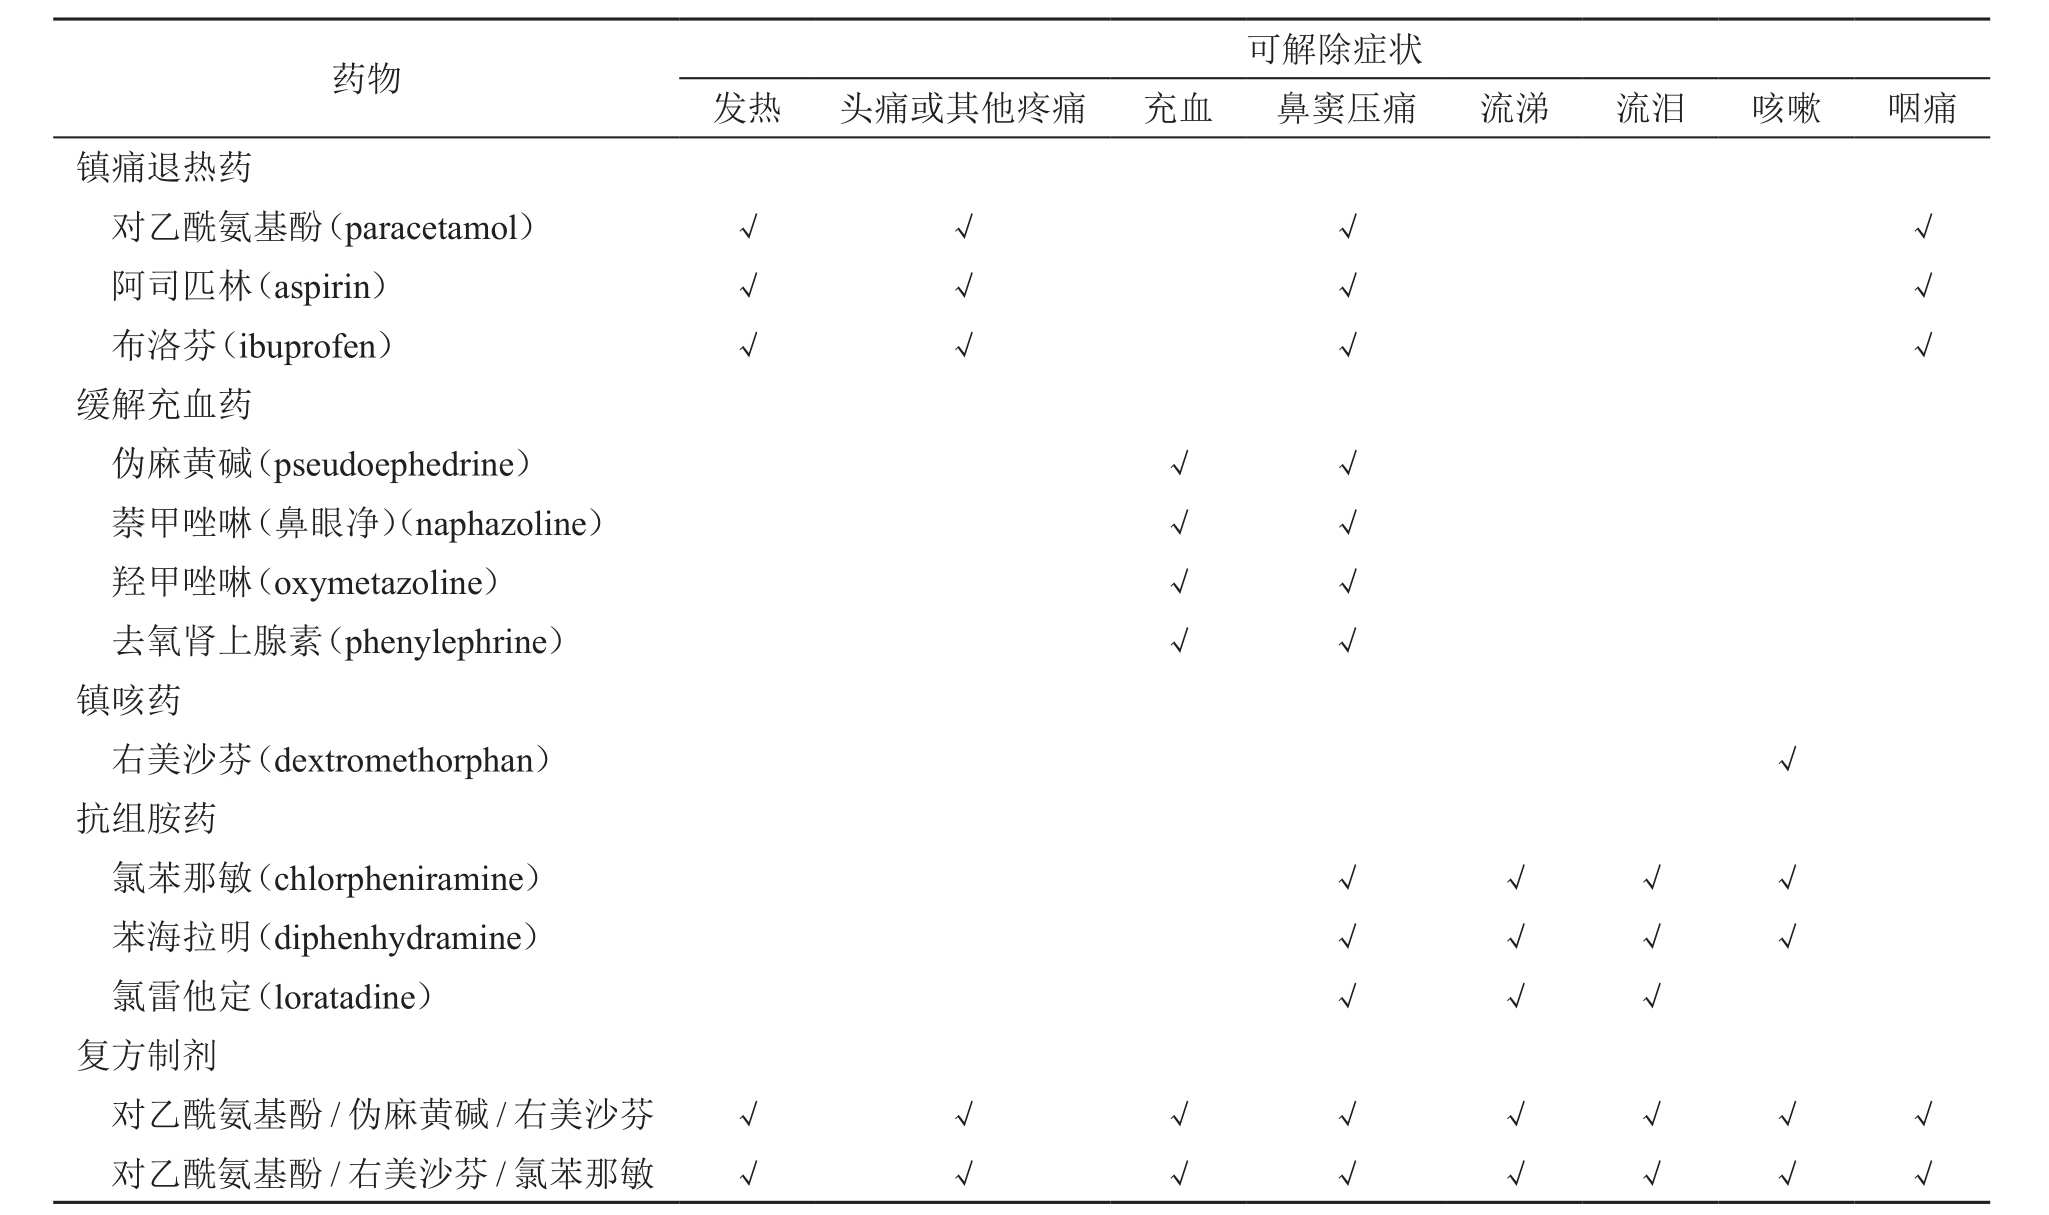
\includegraphics[width=6.82292in,height=4.04167in]{./images/Image00363.jpg}
\end{center}

{\small
注:①早期应用抗化学治疗药物大多能较快缓解流感症状,对症状不重者不一定使用上述药物,对年老体弱者应警惕镇痛退热引起出汗过多和虚脱;②儿童忌用阿司匹林(包括阿司匹林或水杨酸制剂),据认为此类药物与流感的肝脏和神经系统并发症即Reye综合征可能存在相关性}
\end{table}



药物预防可使用金刚烷胺100mg口服,每天2次,连服10~14天,仅对甲型流感有一定预防作用;奥司他韦成人预防用药为75mg口服,每天1次,连服7天。

\protect\hypertarget{text00212.html}{}{}

\hypertarget{text00212.htmlux5cux23CHP7-1-5}{}
参 考 文 献

1.
中华医学会呼吸病分会.流行性感冒临床诊断和治疗指南(2004年修订稿).中华结核和呼吸杂志,2005,28(1):5

2. 杨绍基,任红.传染病学.第7版.北京:人民卫生出版社,2008:62

3. 李梦东,王宇明.实用传染病学.第3版.北京:人民卫生出版社,2004:295

\protect\hypertarget{text00213.html}{}{}

\chapter{人 禽 流 感}

人禽流感(human avian
influenza)是由甲型流感病毒某些感染禽类亚型中的一些毒株引起的急性呼吸道传染病。人禽流感的主要临床表现为高热、咳嗽和呼吸急促,病情轻重不一,其中高致病性禽流感(highly
pathogenic avian influenza,HPAI)常由H\textsubscript{5}
N\textsubscript{1}
亚型引起,病情严重,可出现毒血症、感染性休克、MODS及Reye综合征等多种并发症,病死率高达60\%。

\subsection{病因与发病机制}

\subsubsection{病原学}

流感病毒根据其特异性核糖蛋白抗原的不同,可区分为甲、乙、丙三个型,其中乙型和丙型只感染人,而甲型流感病毒不仅在人类中流行,而且在动物中尤其是禽类中广泛流行。甲型流感病毒表面有两种蛋白质抗原,即血凝素(H)及神经氨酸酶(N)。H抗原又分为16个亚型(H\textsubscript{1}
~H\textsubscript{16} ),N抗原可分为9个亚型(N\textsubscript{1}
~N\textsubscript{9}
)。所有这些亚型都可以感染禽,但引起禽大流行的只是其中某些亚型,特别是H\textsubscript{5}
和H\textsubscript{7} 亚型中的一些高致病毒株如H\textsubscript{5}
N\textsubscript{1} 及H\textsubscript{7} N\textsubscript{1}
等。引起人禽流感的毒株目前已知除H\textsubscript{5} N\textsubscript{1}
外还有H\textsubscript{7} N\textsubscript{3} 、H\textsubscript{7}
N\textsubscript{7} 、H\textsubscript{9} N\textsubscript{2}
等。但这些亚型对人致病性不同,如H\textsubscript{5} N\textsubscript{1}
对人致病性大,而H\textsubscript{7} N\textsubscript{7}
仅引起人的结膜炎,H\textsubscript{9} N\textsubscript{2}
则仅为轻微上呼吸道症状。致病性大小与HN抗原裂解位点上碱性氨基酸数量有关,氨基酸多则致病性大。

禽流感病毒像一般流感病毒一样具有容易变易的特性。H\textsubscript{5}
N\textsubscript{1}
在1959年苏格兰首次发现,但当时仅感染禽而不感染人,但到1997年香港就感染人了。这说明它已突破了种族屏障。另外H\textsubscript{5}
N\textsubscript{1}
在1997年对鸭仅是感染而不发病,但到2003年其毒力发生变化,它不仅对鸭感染而且还发病。其次禽流感病毒的易变性还在于它的基因分节段,宿主范围又广,所以有基因重配的可能性。如果它长期在人群中传播,某些人既感染了禽流感又同时感染了人流感,病毒就会产生基因重配,形成新的亚型毒株,这种病毒既有很高的致病性又具有在人间传播的能力,就可能在人间造成一次新的流感大流行,后果就不堪设想。某些禽流感病毒与人流感病毒也可以同时感染猪,在猪中形成重配株,再感染人也可造成新变异株在人间大流行。

禽流感病毒室温下在粪便中可存活1周,在水中可存活1个月。对pH <
4.1条件下也可存活。它对低温抵抗力强,4℃下可生存30~50天,在羽毛中也可活18天,在冷冻的禽肉和骨髓中可存活10个月之久。禽流感病毒对热敏感,加热到65℃、30分钟或煮沸(100℃)2分钟就会灭活。在直射阳光下40~48小时灭活,用紫外线直接照射可迅速破坏其活性。病毒对常用消毒剂都敏感,如氧化剂、卤素化合物、稀酸等都能迅速破坏其活性。

\subsubsection{发病机制}

人禽流感的发病机制与普通流感的发病机制基本一致。病理解剖显示,支气管黏膜严重坏死;肺泡内大量淋巴细胞浸润,可见散在的出血灶和肺不张;肺透明膜形成。

\subsection{诊断}

\subsubsection{流行病学}

人禽流感的传染源是感染禽流感病毒的各种家禽,主要是鸡和鸭(包括火鸡、珍珠鸡和鹅)。至于家禽的流感最早是如何来的?现在的研究认为是从候鸟等野水禽传播的。某些野水禽及野鸟中都能分离到禽流感病毒。大部分野鸟与野水禽只是感染而不发病,但它们的粪便等排泄物中却有病毒,通过气溶胶或污染的水传播给家禽,家禽受染后其中的某些高致病毒株可使其很快发病,使鸡全身发绀,身体蜷缩,严重黏便、神经失调、严重中毒,肝脾肺等全身器官均染有病毒,病鸡常在48小时内迅速死亡。但鸭子感染后常无症状但全身还带菌仍起着传染源的作用。由于病鸡的血液、肌肉、骨髓、内脏、粪便等各种排泄物中存在大量病毒,除了迅速在鸡群中传播外,人们在饲养、清洁禽舍、屠宰、处理、准备烹调过程中直接接触禽及其内脏,或被其粪便污染的各种物品,通过消化道与被污染的空气吸入呼吸道而感染。有时也可经眼结膜或破损皮肤感染。各年龄群均为易感者。虽然有疑似人传人的报告但至今未被证实。禽流感一般在秋冬及早春季节多见,特别是候鸟迁徙季节。但如果发生在禽流感病毒实验室,因接触毒株而感染则无季节性,随时可发生。从事家禽养殖业者,在发病前1周内去过家禽饲养、销售及宰杀等场所者以及接触禽流感病毒感染材料的实验室工作人员为高危人群。

\subsubsection{临床特征}

\paragraph{临床表现特点}

禽流感病毒感染人的潜伏期一般为1~4天,平均3天,通常不超过7天。不同亚型的禽流感病毒感染人类后可引起不同的临床症状。感染H\textsubscript{9}
N\textsubscript{2}
亚型的患者通常仅有轻微的上呼吸道感染症状,部分患者甚至无任何症状;感染H\textsubscript{7}
N\textsubscript{7}
亚型的患者主要表现为结膜炎;重症患者一般均为H\textsubscript{5}
N\textsubscript{1} 亚型的病毒感染。高致病性禽流感H\textsubscript{5}
N\textsubscript{1}
的症状:起病急,早期表现类似一般流感,发热,大多持续38.5~40℃以上,热程1~7天,一般为3~4天。伴有流涕、鼻塞、咳嗽、咽痛、头痛、肌肉酸痛、全身不适。但病程进展迅速,很快有肺炎表现,肺部有实变体征。严重者呼吸困难,出现急性呼吸窘迫综合征(ARDS),肺出血,胸腔积液及Reye综合征,肾功能衰竭、败血症及休克而很快死亡。部分患者可有恶心、腹痛、腹泻、稀水样便等消化系统症状。极少数患者只有腹泻及昏迷的表现。

\paragraph{实验室检查}

①外周血象:白细胞总数一般不高或降低,但淋巴细胞常减少,部分患者白细胞总数及淋巴细胞数均减少。血小板数也可减少。少数患者全血细胞减少。②病毒抗原及基因检测:早期取患者鼻咽分泌物等呼吸道标本,采用免疫荧光或酶联免疫法检测甲型流感病毒核蛋白抗原(NP)、M\textsubscript{1}
蛋白抗原及禽流感病毒H亚型抗原。还可用A(H\textsubscript{5}
N\textsubscript{1}
)特异血凝素基因以RT-PCR法检测禽流感病毒亚型特异性H及N抗原基因。③病毒分离:患者呼吸道标本(如鼻咽分泌物、口腔含漱液、气管吸出物或呼吸道上皮细胞)用鸡胚或MDCK细胞培养分离禽流感病毒。④血清学检查:用血凝抑制试验或酶联免疫等血清学方法检查发病初期和恢复期双份血清,抗禽流感病毒抗体呈4倍或以上升高有助于回顾性诊断。

\paragraph{胸部影像学检查}

H\textsubscript{5} N\textsubscript{1}
亚型病毒感染者可出现肺部浸润,肺内片状影。重症患者肺内病变进展迅速,呈大片毛玻璃状影及肺实变影像。病变后期为双肺弥漫性实变,少数可合并胸腔积液。

\subsubsection{诊断标准}

根据流行病学接触史(即:①发病前1周内曾到过疫点,有感染禽流感病毒的可能;②与被感染的家禽及其分泌物、排泄物等有密切接触史者;③与禽流感患者有密切接触史者有患病的可能)、临床表现及实验室检查结果,可作出人禽流感的诊断。流行病学接触史在诊断中具有重要意义。

\paragraph{医学观察病例}

在病前1周内到过疫点、与被感染家禽或其排泄物或可疑禽流感患者有流行病学接触史,1周内出现流感样临床表现者定为医学观察病例。

对于被诊断为医学观察病例者,医疗机构应及时向当地疾病预防控制机构按预警病例报告,并隔离观察7天。

\paragraph{疑似病例}

有流行病学接触史和临床表现,患者呼吸道分泌物标本甲型流感病毒H亚型抗原检测阳性或核酸检测阳性者。

\paragraph{临床诊断病例}

疑似病例排除其他诊断,无法进一步取得实验室证据,与其有共同接触史的患者已被诊断为确诊病例者。

\paragraph{确诊病例}

有流行病学接触史和临床表现,从患者呼吸道分泌物标本中分离出特定病毒或采用RT-PCR法检测到禽流感H亚型病毒基因,且发病初期和恢复期双份血清抗禽流感病毒抗体滴度4倍或以上升高者。

\subsubsection{诊断注意事项}

临床应注意与流感,普通感冒,细菌、支原体、衣原体、军团菌性肺炎,传染性单核细胞增生症,SARS,巨细胞病毒及肺炎型流行性出血热等病毒性肺炎进行鉴别,鉴别主要依靠病原学检查。

\subsection{治疗}

1.对疑似和确诊患者应进行隔离治疗。

2.对症治疗
可应用解热药、缓解鼻黏膜充血药、止咳祛痰药等。儿童忌用阿司匹林或含阿司匹林以及其他水杨酸制剂的药物,避免引起儿童Reye综合征。

3.抗病毒治疗 应在发病48小时内试用抗流感病毒药物。

(1)
神经氨酸酶抑制剂:通过抑制流感病毒的神经氨酸酶来抑制病毒复制,同时减弱病毒的致病力。奥司他韦(oseltamivir,达菲)是目前WHO确认和推荐的人禽流感预防治疗药物,对禽流感病毒H\textsubscript{5}
N\textsubscript{1} 和H\textsubscript{9} N\textsubscript{2}
亚型均有抑制作用,对耐金刚烷胺和金刚乙胺的禽流感病毒仍有效。成人剂量每日150mg,儿童剂量每日3mg/kg,分2次口服,疗程5天。本品能减轻症状,缩短病程,减少并发症。

(2) 离子通道M\textsubscript{2}
阻滞剂:该类药物主要通过干扰病毒M\textsubscript{2}
离子通道活性来抑制禽流感病毒株的复制,早期应用可阻止病情发展、减轻病情、改善预后。金刚烷胺(amantadine)成人剂量每日100~200mg,儿童每日5mg/
kg,分2次口服,疗程5天。肾功能受损者酌减剂量。治疗过程中应注意中枢神经系统和胃肠道副作用。老年患者及孕妇应慎用,哺乳期妇女、新生儿和1岁以下婴儿禁用。金刚乙胺(rimantadine)用量同金刚烷胺,但每日仅需服用1次,毒副作用相对较轻。某些毒株可能对金刚烷胺和金刚乙胺有耐药性。

4.中医药治疗

(1)
辨证论治:①轻证:毒犯肺胃。症状:发热,恶寒,咳嗽,少痰,咽痛,头痛,肌肉关节酸痛,部分患者伴有恶心,呕吐,腹泻,舌苔白、白腻或黄腻,脉浮滑数。病机:疫毒之邪袭于肺胃,致肺胃蕴邪,肺失宣肃,胃肠失和,湿热壅滞。治法:清热解毒,宣肺化湿,调和胃肠。参考处方:桑叶、菊花、炒杏仁、黄连、连翘、知母、生石膏、藿香、佩兰、苍术、姜半夏、芦根。加减:口干者加沙参;咳嗽甚者加枇杷叶、浙贝母;苔腻甚者加草果;恶心呕吐者加竹茹、苏叶;腹泻者去知母,加马齿苋。②重证:疫毒壅肺,内闭外脱。症状:高热,寒战,咳嗽,少痰难咳,胸痛,憋气喘促,口唇紫暗,或心悸,四末不温,冷汗淋漓,躁扰不安,甚则神昏谵语,舌暗红苔黄腻或灰腻,脉细数或脉沉细欲绝。病机:疫毒之邪壅肺,热毒壅盛,故高热,寒战;肺失宣降,故喘息憋气;痰瘀闭肺,肺气欲绝,故呼吸极度困难,喘息气促,阳气欲脱,可见心悸、心慌,四肢末发冷,冷汗淋漓等。治法:清肺解毒,扶正固脱。参考处方:炙麻黄、生石膏、炒杏仁、知母、川贝母、鱼腥草、黄芩、葶苈子、虎杖、西洋参、山萸肉、炙甘草。加减:高热、神志恍惚,甚则神昏谵语者上方送服安宫牛黄丸(或胶囊),也可选用清开灵、醒脑静、鱼腥草注射液。肢冷、汗出淋漓者去川贝母,加桂枝、干姜、炮附子、煅龙骨、煅牡蛎,注射剂可选用生脉注射液、参麦注射液、参附注射液、黄芪注射液等。口唇发绀加三七、益母草、黄芪、当归尾;苔黄腻甚者加藿香、佩兰、黄连。

(2)
中成药应用:应当辨证使用口服中成药或注射剂,可与中药汤剂配合应用。①解表清热类:可选用柴银口服液、银黄颗粒等。②清热解毒类:可选用双黄连口服液、清热解毒口服液(或颗粒)等。③清热开窍类:可选用安宫牛黄丸(或胶囊)、清开灵口服液(或胶囊)等。④清热祛湿类:可选用藿香正气丸(或胶囊)、葛根芩连微丸等。以上4类均可选用清开灵注射剂、醒脑静注射液、鱼腥草注射剂、双黄连粉针剂等。⑤扶正固脱类:可选用生脉注射液、参麦注射液、参附注射液、黄芪注射液等;也可配合使用生脉饮口服液、百令胶囊、金水宝胶囊等。

5.加强支持治疗和预防并发症
注意休息、多饮水、增加营养,给易于消化的饮食。密切观察,监测并预防并发症。抗菌药物应在明确继发细菌感染时或有充分证据提示继发细菌感染时使用。

6.重症患者的治疗
重症患者或发生肺炎的患者应入院治疗,对出现呼吸功能障碍者给予吸氧及其他相应呼吸支持,发生其他并发症的患者应积极采取相应治疗。

\subsection{预后}

人禽流感预后与感染的病毒亚型有关,感染H\textsubscript{9}
N\textsubscript{2} 、H\textsubscript{7} N\textsubscript{3}
、H\textsubscript{7} N\textsubscript{7}
者,大多数预后良好。而感染H\textsubscript{5} N\textsubscript{1}
者预后较差。影响预后的因素还与患者年龄、是否有基础疾病、治疗是否及时以及是否有并发症等有关。

\protect\hypertarget{text00214.html}{}{}

\hypertarget{text00214.htmlux5cux23CHP7-2-5}{}
参 考 文 献

1. 中华人民共和国卫生部 .人禽流感诊疗方案(2005年修订版).

2. 杨绍基,任红.传染病学.第7版.北京:人民卫生出版社,2008:66

\protect\hypertarget{text00215.html}{}{}

\chapter{流行性腮腺炎}

流行性腮腺炎(epidemic
parotitis,mumps)是由腮腺炎病毒所引起的急性呼吸道传染病。其特征为腮腺的非化脓性肿胀、疼痛、发热伴咀嚼受限,可延及各种腺组织或中枢神经系统及肝、肾、心脏等器官而引起相应的症状。好发于儿童、青少年甚至成人中的易感者。患儿易并发脑膜脑炎,成人患者易并发睾丸炎或卵巢炎以及其他涎腺的非化脓性炎症。预后良好,病死率为0.5\%~2.3\%,主要死于重症腮腺炎病毒脑炎。

\subsection{病因与发病机制}

腮腺炎病毒(mumps
virus)属副黏液病毒,是单股RNA病毒,呈球形,直径为100~200nm。仅一个血清型,病毒外膜具有血凝素抗原(V)和位于核壳的可溶性抗原(S),人感染后体内可出现相应的V和S抗体,均可用补体结合试验检测。自然界中人是本病毒唯一宿主。此病毒抵抗力不强,对一般化学及物理消毒剂均很敏感,紫外线照射下迅速死亡。4℃时其活力可保持2个月,一般室温中2~3天传染性即消失,加热至55~60℃,经过10~20分钟失去活力。传染源主要为早期患者和隐性感染者,自腮腺肿大前7天至肿大后9天约2周时间内均有传染性。借飞沫和密切接触传染。全年均可发病,但以冬、春季为主,患者主要为学龄儿童,无免疫力的成人亦可发病。一次得病后(包括隐性感染和无腮腺肿大者在内)可获得持久免疫,再感染者极少见。

病毒从呼吸道侵入人体后,在局部黏膜上皮细胞和局部淋巴结中增殖,然后侵入血液循环(第一次病毒血症),经血流累及腮腺、中枢神经系统和其他一些器官,在其中增殖复制,然后再次进入血液循环(第二次病毒血症),并可侵犯第一次未受波及的脏器,如颌下腺、舌下腺、睾丸、胰腺等,引起相应的临床表现。因此流行性腮腺炎实际上是一种系统性、多器官受累的疾病,临床表现形式多样。病理特征为腮腺非化脓性炎症,颌下腺及其他腺体如睾丸、卵巢、胰腺、乳腺、胸腺、甲状腺等也可受累。胰腺受累时血及尿中淀粉酶含量增加。脑组织病变可呈急性病毒性脑膜脑炎改变等。

\subsection{诊断}

\subsubsection{流行病学特点}

全年均可发病,但以冬春季为高峰,呈流行或散发,于2~3周前有与流行性腮腺炎患者接触史。

\subsubsection{临床表现特点}

潜伏期14~25天,平均18天。多数病例无前驱症状而以耳下部肿大为最早表现。少数患者有前驱症状如畏寒、发热、头痛、纳差、全身不适等,数小时或1~2天后腮腺即逐渐明显肿大,此时体温可上升达39℃以上,甚至40℃,成人患者症状一般较重。腮腺肿大以耳垂为中心,向前、后、下发展,边缘不清,同时伴有周围组织水肿,局部皮肤紧张发亮,但无明显发红,无化脓,具有弹性感,表面灼热并有触痛,张嘴、咀嚼或进酸味饮食时疼痛加重(因腮腺管发炎、部分阻塞,故进酸性食物促进腺体分泌而疼痛加剧)。通常先一侧腮腺肿1~4天(偶尔1周以上),然后对侧也肿大,但也有双侧同时肿大。肿胀于2~3天达高峰,再持续4~5天后逐渐消退,全程10~14天。双侧腮腺均肿胀者约占70\%~75\%。腮腺肿胀时或肿胀前后,颌下腺和舌下腺亦可被累及。颌下腺肿大时颈部明显肿胀,颌下可扪及柔软而具轻触痛的椭圆形腺体;舌下腺肿大时可见舌及颈部肿胀,严重者引起吞咽困难。腮腺四周的组织也呈水肿,可上达颞部及颧骨弓,下达颌部及颈部,甚至波及胸锁乳突肌。有时可伴胸骨前水肿,因而使面貌变形。腮腺管口(位于上颌第二臼齿对面黏膜上)在早期可红肿,有助于诊断。

本病可有以下几种并发症:

\paragraph{神经系统并发症}

①脑膜炎、脑膜脑炎:有症状的脑膜炎发生在15\%的病例,为小儿患者中最常见的并发症,可发生于腮腺肿大前6~7天至腮腺肿大后2周内,大多数在腮腺肿后1周内出现。有的患者脑膜炎先于腮腺炎。主要表现有头痛、嗜睡和脑膜刺激征,一般症状在1周内消失,预后良好。脑膜脑炎或脑炎患者,常有高热、谵妄、抽搐、昏迷,重症者可致死亡。可遗留耳聋、视力障碍等后遗症。②多发性神经炎:偶于腮腺炎后1~3周内发生。此外尚可有暂时性面神经麻痹、平衡失调、三叉神经炎、偏瘫、截瘫、上升性麻痹等。预后多良好。

\paragraph{胰腺炎}

成人中约占5\%,儿童中较少见。常发生于腮腺肿大后3~7天内。因腮腺炎本身可引起淀粉酶增多,故测定血清脂肪酶价值更大。

\paragraph{生殖系统并发症}

成人男性14\%~35\%可并发睾丸炎,常见于腮腺肿大开始消退时患者又出现发热,睾丸明显肿胀和疼痛,可并发附睾炎、鞘膜积液和阴囊水肿。睾丸炎多为单侧,约1/3的病例为双侧。急性症状持续3~5天,10天内逐渐好转。部分患者睾丸炎后发生不同程度的睾丸萎缩,这是病毒引起睾丸细胞坏死所致,但很少引起不育症。幼年患者很少发生睾丸炎。成人女性中5\%~7\%合并卵巢炎,一般不影响生育能力。

\paragraph{肾炎}

轻者仅有少量蛋白尿或血尿,重者与急性肾炎的表现及过程相同,多数预后良好。个别严重者可发生急性肾功能衰竭,甚至死亡。

\paragraph{心肌炎}

约4\%~5\%患者发生心肌炎,多见于病程的5~10天,严重者可致命。但大多数仅有心电图改变而无明显临床症状。

\paragraph{其他}

乳腺炎、甲状腺炎、胸腺炎、血小板减少、荨麻疹、急性滤泡性结膜炎等均少见。关节炎发生率为0.44\%,主要累及肘、膝关节等大关节,可持续2天至3个月不等,能完全恢复。多发生于腮腺肿大后1~2周内,也有无腮腺肿大者。

少数不典型病例可始终无腮腺肿胀,而以单纯脑膜脑炎、睾丸炎的症状出现,也有仅见颌下腺或舌下腺肿胀者。

\subsubsection{实验室检查}

\paragraph{血象}

白细胞总数多正常或稍增加,淋巴细胞相对增多。伴有并发症时白细胞总数可增高。

\paragraph{血 、尿淀粉酶}

90\%的患者血清淀粉酶在早期有轻~中度增高。尿中淀粉酶值亦增高。酶值增高程度往往与腮腺肿胀程度成正比,但也可能与胰腺受累等有关。

\paragraph{血清学检查}

补体结合试验和血凝抑制试验,双份血清效价增高4倍以上有诊断价值。近年来用酶联免疫吸附法及间接荧光免疫检测IgM抗体,以及用单克隆抗体检测患者血清、唾液中的腮腺炎病毒抗原,二者均可作早期诊断。对一般急诊患者,不必依靠血清学检查,若为除外或证实无唾液腺肿大的并发症,以及鉴别其他病毒性腮腺炎时,则需做血清学检查。

\paragraph{病毒分离}

早期病例,唾液、尿液、血、脑脊液以及脑、甲状腺等其他组织中可分离出病毒。

\subsubsection{诊断注意事项}

本病主要根据典型的非化脓性腮腺肿大、有发热等急性起病的临床经过,结合当地流行情况和病前2~3周有接触患者史,诊断并不困难。无腮腺肿大的脑膜炎、脑膜脑炎和睾丸炎等,确诊需依靠血清学检查和病毒分离。

此外,本病尚应与下列疾病进行鉴别:

\paragraph{化脓性腮腺炎}

本病常为一侧性腮腺肿大,不伴睾丸炎或卵巢炎。肿大的腮腺表现红、肿、痛、热均明显,严重时可有波动感,挤压腮腺时腮腺导管口常可见到脓液流出。外周血白细胞总数、中性粒细胞均明显增高,有核左移现象。

\paragraph{颈 、耳前或颌下淋巴结炎}

淋巴结肿大不以耳垂为中心,而是在相应淋巴结的部位。边缘清楚,质地坚硬,唾液腺导管口无明显改变。外周血白细胞总数、中性粒细胞均增高。

\paragraph{其他病毒所致的腮腺肿大}

已知许多病毒如副流感病毒、流感病毒、巨细胞病毒、肠道病毒等均可引起腮腺肿大。仅从临床表现不易与流行性腮腺炎相鉴别,需靠特异性血清学检查或病毒分离才能鉴别。

\paragraph{症状性腮腺肿大}

糖尿病、慢性肝病、营养不良、结节病、腮腺导管阻塞等,以及青春期男性均可有单纯性腮腺肿大。服用碘化物、保泰松、硫氧嘧啶等也可引起腮腺肿大,呈对称性,质软,无肿痛感。不伴急性感染症状,局部也无明显疼痛和压痛。

\subsection{治疗}

本病目前尚无特效治疗,一般采取中西医结合方法对症处理。

\paragraph{一般治疗}

呼吸道隔离及卧床休息,应隔离至热退、腮腺肿大完全消失之后。同时加强口腔护理,以复方硼砂液漱口,保持口腔清洁。饮食以流质软食为宜,应避免进酸味饮料及食物,以减少唾液腺的分泌。高热不退可用物理降温,或用退热药物如APC片等。

\paragraph{中医中药治疗}

以清热解毒、软坚消痈治疗为主。局部用紫金锭或青黛散调醋外敷,1日数次;或金黄散、芙蓉叶各30g研末,菊花9g浸汁加蜜糖适量拌和,每日2次外敷;或蒲公英、鸭跖草、水仙花根、马齿苋等捣烂外敷,可减轻疼痛。内服普济消毒饮方为主,随证加减。也可口服板蓝根冲剂1~2袋,每日2~3次,或肌内注射板蓝根注射液2ml,每日1~2次。

\paragraph{氦氖激光局部照射}

能减轻局部胀痛,并可缩短局部肿胀时间。

\paragraph{抗病毒治疗}

早期可使用利巴韦林(病毒唑)、成人每日0.75~1.0g,儿童15mg/kg静脉滴注,疗程5~7天,可缩短病程及减少并发症发生。干扰素使用亦有报道。

\paragraph{肾上腺皮质激素}

一般患者尽量不用,但对重症患者如有高热不退、对一般降温处理无效或合并严重中枢神经系统并发症、心肌炎、严重的睾丸炎或胰腺炎等,可考虑短期(5~7天)应用。

\paragraph{并发症的治疗}

①脑膜脑炎时按病毒性脑炎处理。②合并睾丸炎时应以丁字带将睾丸托起,以减轻疼痛,局部间歇冷敷,必要时可用镇痛剂。如疼痛剧烈不能

忍受时,可以普鲁卡因作精索封闭。③心肌炎时应绝对卧床休息,并按心肌炎常规治疗。④并发胰腺炎时应禁食,并按胰腺炎常规处理。⑤预防睾丸炎:男性成人患者在本病早期应用己烯雌酚1mg/次,每日3次口服,可能有预防睾丸炎发生的作用。

\protect\hypertarget{text00216.html}{}{}

\hypertarget{text00216.htmlux5cux23CHP7-3-4}{}
参 考 文 献

1. 杨绍基,任红.传染病学.第7版.北京:人民卫生出版社,2008:79

2. 陈灏珠,林果为.实用内科学.第13版.北京:人民卫生出版社,2009:405

\protect\hypertarget{text00217.html}{}{}

\chapter{麻 疹}

麻疹(measles,rubeola)是由麻疹病毒引起的急性呼吸道传染病,临床以发热、咳嗽、流涕、眼结膜充血、颊黏膜有麻疹黏膜斑及皮肤出现红色斑丘疹等为主要表现。任何年龄均可感染麻疹,但过去一般以8个月以上到5岁小儿发病率最高,每隔2~3年有一次大流行。自1965年普遍接种麻疹减毒活疫苗后,变为局部暴发流行或散发;发病年龄也向后推移,青少年及成人发病率相对上升,5岁以下学龄前儿童约占48.1\%,而20岁以上成人可达22.5\%。任何季节均可发病,以冬春季为最多。

\subsection{病因与发病机制}

麻疹病毒属副黏液病毒科,呈球形,直径为150~200nm。病毒核心为由负股单链RNA和三种核衣壳蛋白(L、P、N蛋白)组成的核壳体,外层为含脂质双层的包膜,表面有细小的糖蛋白突起。外膜中的蛋白成分主要有膜蛋白(M蛋白)、血凝素(H蛋白)和融合蛋白(F蛋白)。M蛋白功能与病毒装配、芽生、繁殖有关。H蛋白含有细胞受体位点,可与宿主细胞表面的麻疹病毒受体(CD\textsubscript{46}
)结合,启动感染过程。F蛋白与病毒血溶活性和细胞融合活性有关,有利于病毒进入细胞和使细胞与细胞融合。F蛋白和H蛋白是麻疹病毒引起人体产生抗体应答的主要抗原。抗H蛋白抗体具有免疫性保护作用,抗F蛋白抗体能阻止细胞间的感染。麻疹病毒可在T淋巴细胞和B淋巴细胞及单核细胞内复制。人为麻疹病毒唯一宿主,患者是本病唯一的传染源,从潜伏期末2~3天至出疹后5天内,眼结膜、鼻、咽、气管的分泌物、尿及血液中均含有病毒,有传染性,恢复期不携带病毒。主要通过喷嚏、咳嗽、说话、哭吵时借飞沫直接传播。人对麻疹普遍易感,凡未患过麻疹又未接种麻疹减毒活疫苗者,一旦接触麻疹患者后,90\%以上发病。病后可获得持久免疫力,第二次患麻疹者极少见。

麻疹病毒借助飞沫,经鼻、口咽、眼结膜等进入体内,首先在鼻咽部、眼结膜和上呼吸道黏膜上皮细胞、黏膜下和局部淋巴结进行繁殖,繁殖后入血,于感染后第2~3天引起第一次病毒血症。病毒随后进入全身单核-巨噬细胞系统中繁殖。感染后第5~7天,大量复制后的病毒再次侵入血流,导致第二次病毒血症。病毒由血白细胞携带播散至全身各组织器官,主要部位有呼吸道、眼结合膜、口咽部、皮肤、胃肠道等,此时出现一系列的临床表现。约病程第15天后,由于机体特异性免疫应答(产生IgG抗体),致病毒被清除,临床进入恢复期。

麻疹时呼吸道黏膜有充血、水肿,毛细血管周围有单核细胞浸润、炎症渗出,出现呼吸道症状。口腔黏膜充血可见到针尖大小灰白小点,形成麻疹黏膜斑(Koplik's
spot),系黏膜及黏膜下炎症、局部充血、渗出、细胞浸润、坏死和角化。在感染过程中,细胞免疫反应逐渐形成,致敏的淋巴细胞释放淋巴因子,引起炎症反应,使受染的细胞增大,融合成多核巨细胞(华-弗细胞,Warthin-Finkeldey
giant
cells),是麻疹特征性的病理改变,可见于皮肤、眼结合膜、呼吸道和胃肠道黏膜、全身淋巴组织、肝、脾等处。皮疹为病毒或免疫损伤致皮肤浅表血管内皮细胞肿胀、增生、渗出,真皮淋巴细胞浸润、充血肿胀所致。由于崩解的红细胞和血浆渗出,使皮疹消退后遗留色素沉着,表皮细胞坏死及退行性变形成脱屑。并发脑炎时脑组织可出现充血、水肿、点状出血或脱髓鞘病变。此外,麻疹感染时对机体免疫系统有暂时抑制,如白细胞、血小板和补体等均有下降,结核菌素阴转患者易继发感染,结核病灶激活或扩散;而哮喘、湿疹、肾病综合征等疾病在麻疹期间可暂时缓解。

\subsection{诊断}

\subsubsection{流行病学资料}

儿童多见。任何季节均可发病,以冬春季为最多。

\subsubsection{临床表现特点}

潜伏期约10天(6~21天),接受过被动免疫者可延长至3~4周。

\hypertarget{text00217.htmlux5cux23CHP7-4-2-2-1}{}
(一) 典型麻疹

疫苗接种免疫失败和未接种疫苗者几乎全部表现为典型麻疹
,继发性免疫失败者中约有1/6左右的人也表现为典型麻疹。典型麻疹临床过程可分为以下三期:

\paragraph{前驱期(卡他期)}

从发热到出疹为前驱期,一般持续约3~4天(1~8天)。此期主要为上呼吸道炎症及眼结合膜炎所致的卡他症状。有发热、咳嗽、喷嚏、流涕、流泪、畏光、结膜充血、眼睑水肿,并有浆液脓性分泌物。起病后第2~3天约90\%患者于双侧近臼齿颊黏膜处出现细小灰白色小点(约0.5~1mm大小),周围有微血管扩张的红晕,称麻疹黏膜斑,为本病早期特征。初起时仅数个,很快增多,且融合扩大成片,似鹅口疮,一般持续到出疹后1~2天内消失。也可见于下唇内侧及牙龈黏膜,偶见于上腭。偶见颈、胸、腹部出现风疹样或猩红热样皮疹,数小时后即消失,称麻疹前驱疹。有时在悬雍垂、扁桃体、咽后壁、软腭处见红色斑点,出疹期始消退,称黏膜疹。在发热同时可伴有全身不适、精神委靡、食欲减退、腹泻、呕吐等症状。

\paragraph{出疹期}

发热3~5天后,当呼吸道症状及体温达高峰时开始出现皮疹。皮疹先见于耳后、发际,逐渐波及头面部、颈部,一日内自上而下蔓延到胸、背、腹及四肢,约2~3天内遍及手心、足底,此时头面部皮疹已可开始隐退。皮疹初为淡红色斑丘疹,大小不等,直径2~5mm,散在分布,继而增多,呈鲜红色,以后逐渐融合成暗红色、形态不规则或小片状斑丘疹,疹间皮肤正常。皮疹为充血性,压之褪色,少数病例皮疹呈出血性。出疹时全身中毒症状加重,体温高达40℃左右,精神委靡、咳嗽频繁,声音嘶哑,畏光、结膜红肿、眼睑水肿。重者可有谵妄、抽搐。全身表浅淋巴结与肝脾可轻度肿大。肺部常有干湿性啰音。本期约3~5天。

\paragraph{恢复期}

皮疹出齐后按出疹顺序依次消退,由红色转为棕褐色,全身症状随着体温下降而迅速减轻,精神与食欲开始好转,皮疹消退后留下特征性的棕褐色色素沉着及糠麸样脱屑,以躯干为多,约1~2周消失。这种色素沉着斑在麻疹后期有诊断价值。无并发症者整个病程约10~14天。

\hypertarget{text00217.htmlux5cux23CHP7-4-2-2-2}{}
(二) 非典型麻疹

由于感染者的年龄不同
、机体的免疫状态不同、病毒毒力的强弱不一、侵入人体数量的不同等因素,临床上可出现以下各种非典型麻疹。

\paragraph{轻型麻疹}

多见于对麻疹病毒有部分免疫力者,如6个月以内婴儿尚留存来自母体的被动免疫抗体,近期接受过免疫制剂(如丙种球蛋白)或接种过麻疹免疫疫苗者,或第二次患麻疹者。其潜伏期较长(3~4周),临床症状轻,麻疹黏膜斑不典型或缺如,皮疹少而色淡,出疹期短,不留色素沉着,较少并发症但有传染性。病后所获免疫力与典型麻疹者相同。

\paragraph{重型麻疹}

多见于全身情况差、免疫力低下,或继发严重感染者,病死率高。包括:①中毒性麻疹:起病急骤,高热40℃以上,严重中毒症状,谵妄或昏迷,反复抽搐,呼吸急促,唇指发绀,脉细速,皮疹密集,呈暗红色且融合成片;②出血性麻疹:皮疹呈出血性,形成紫斑,压之不褪色,同时可伴内脏出血;③疱疹性麻疹:皮疹呈疱疹样,可融合成大疱。高热、严重中毒症状;④休克性麻疹:皮疹少或皮疹突然隐退,遗留少数皮疹呈青紫色,面色苍白或青灰色,大多因心功能不全或循环衰竭引起。

\paragraph{成人麻疹}

目前成人麻疹发生率已明显上升,与小儿相比中毒症状较重,但并发症较少。临床特点起病急,可无卡他症状,发病第1天即高热,伴有头痛、全身乏力、萎靡不振、纳呆等;而后热型不规则或为稽留热,咳嗽较剧,发病后3~4天出现粗大的斑丘疹,融合,自上而下顺序出现,3~4天后逐渐消退,但留有色素沉着。麻疹黏膜斑十分常见但不典型,消失较晚。妊娠初期发病可致流产,孕期中得病可致死胎。孕妇产前7~10天感染麻疹,则小儿娩出时可无任何症状,而出生后可与母亲同时发生症状;若孕妇产前2周受感染,产时正患麻疹,则小儿出生时可见麻疹,称为先天性麻疹。

\paragraph{非典型麻疹综合征(atypical measles syndrome,AMS)}

又称异型麻疹。主要见于接种麻疹灭活疫苗后4~6年再接种麻疹灭活疫苗,或再接触麻疹患者者,偶见于曾接受减毒活疫苗者。急起高热、头痛、肌痛、乏力等,中毒症状重而卡他症状少,罕见麻疹黏膜斑。起病2~3天后出现皮疹,但从四肢远端开始,逐渐波及躯干与面部,皮疹为多形性,有斑丘疹、疱疹、紫癜或荨麻疹,一般可同时见于2~3种皮疹形态。常伴有四肢水肿、肺炎、胸腔积液,肺内阴影可持续数月至1~2年。血中嗜酸性粒细胞增多,有些患者有肝脾肿大,肢体麻木、无力和瘫痪。诊断依据为恢复期麻疹抗体上升,血凝抑制抗体和补体结合抗体可呈强阳性。可能系人体对麻疹病毒的迟发性变态反应,或抗原抗体复合物沉积于血管基膜引起Arthus反应所致。无传染性。国内均用麻疹减毒活疫苗,故此型极少见。

\subsubsection{并发症}

年幼体弱、营养不良及免疫力低下者,患麻疹后极易发生并发症,常见的有:

\paragraph{肺炎}

除麻疹病毒本身可引起巨细胞肺炎外,在病程各期尚易并发继发性肺炎,为麻疹最常见的并发症,也是麻疹死亡的主要原因。多见于5岁以下的小儿,病原常为金黄色葡萄球菌、肺炎球菌、腺病毒等。大多发生在出疹期,全身中毒症状严重,有高热、咳嗽、气急、鼻翼扇动、唇指(趾)发绀,肺部有中、小细湿啰音。金黄色葡萄球菌感染尤易并发肺脓肿、脓胸或脓气胸、心包炎等,若病程迁延不愈,可导致支气管扩张症。

\paragraph{喉炎}

以2~3岁以下小儿多见。麻疹患者常有轻度喉炎,出现声音嘶哑,有刺激性干咳,预后良好。继发性喉炎多由金黄色葡萄球菌或溶血性链球菌引起,有声嘶加重、犬吠样咳嗽、吸气性呼吸困难(可见三凹征:胸骨上窝、锁骨上窝、肋间隙内陷);严重者有面色苍白、发绀、气促、烦躁,如不及时抢救,可因喉梗阻引起窒息而死亡。

\paragraph{心肌炎 、心功能不全}

重症麻疹因高热、中毒症状严重,可影响心肌功能,尤其在营养不良小儿及并发肺炎时。主要表现为气急烦躁、面色苍白、四肢发绀、脉细速、心率快、心音弱、肝脾肿大,心电图示T波和S-T段改变。病情重危。

\paragraph{脑炎及亚急性硬化性全脑炎(subacute sclerosing panencephalitis,SSPE)}

麻疹并发中枢神经系统病变较其他出疹性疾病为多。麻疹脑炎的发病率为0.1\%~0.5\%,主要为儿童,多发生于出疹后2~6天,偶见于前驱期或出疹后2~3周内。可能为麻疹病毒直接侵入脑组织或(和)与神经组织变态反应有关。临床上有高热、头痛、嗜睡、抽搐、意识障碍、昏迷、呼吸衰竭、强直性痉挛瘫痪、脑膜刺激征和病理反射征阳性。脑脊液细胞数增加(多为单核细胞),蛋白质稍增,糖正常。少数脑脊液亦可正常。病死率约15\%,多数患者经1~5周恢复,部分患者可留有瘫痪、智力障碍、癫痫、失明等后遗症。SSPE是麻疹的远期并发症,但很少见。表现为亚急性进行性脑组织退变,脑组织中能分离出麻疹病毒,血清和脑脊液的麻疹抗体持续强阳性。本病可能系麻疹病毒长期隐伏于脑组织中,产生缺失M膜蛋白的缺陷病毒颗粒所致,也有认为系基因突变致病毒RNA复制障碍而发生结构蛋白变异引起,从而引起脑部进行性退化病变。故目前认为这是一种类麻疹病毒(measleslike
virus)或麻疹有关病毒(measles related
virus)所引起的亚急性或慢性脑炎。潜伏期约2~17年(平均7年),发病年龄以5~15岁儿童为多,多发于男孩。患者逐渐出现智力减退,性格异常,运动不协调,各类癫痫发作,视觉、听觉及语言障碍,共济失调或局部强直性瘫痪,病情发展直至神志不清,呈去大脑强直状态。总病程约1年余,最后死于营养不良、恶病质及继发感染。

\paragraph{肝损害}

多见于成人,重症麻疹患者,肝损害尤甚。肝损害多见于麻疹急性期,即病程的第5~10天,临床表现可有厌食、恶心、腹胀、腹痛、乏力及黄疸等,肝脾肿大,肝脏酶学增高。肝功能大多于2~4周内恢复正常。

\paragraph{其他并发症}

尚可并发口腔炎、中耳炎、乳突炎,大多为细菌继发感染。常因慢性腹泻、照顾不当、忌口等引起营养不良及各种维生素缺乏症。此外尚有结核感染恶化或播散,而致粟粒结核或结核性脑膜炎。

\subsubsection{实验室检查}

\paragraph{血象}

白细胞计数减少,淋巴细胞相对增加;若白细胞计数增加,尤其是中性粒细胞增加,提示继发细菌感染;若淋巴细胞严重减少,提示预后不良。

\paragraph{分泌物涂片检查多核巨细胞}

鼻咽、眼分泌物及尿沉渣涂片,以瑞氏染色,显微镜下可见脱落的上皮多核巨细胞。在出疹前后1~2天即可阳性,比麻疹黏膜斑出现早,有早期诊断价值。

\paragraph{血清学检查}

酶联免疫吸附试验(ELISA)测定血清特异性IgM抗体是诊断麻疹的标准方法,且在发病后2~3天即可测到,因此还具有早期诊断价值。恢复期血清血凝抑制抗体及补体结合抗体有4倍以上增高或发病1个月后抗体滴度大于1∶60,但只能作为回顾性诊断。

\paragraph{病毒学检查}

①病毒抗原检测:应用荧光标记特异抗体检测鼻黏膜印片及尿沉渣,可在细胞内找到麻疹抗原,阳性有诊断价值。②病毒分离:早期从鼻咽部及眼分泌物和血液中分离到麻疹病毒即可肯定诊断。③核酸检测:采用反转录聚合酶链反应(RT-PCR)从临床标本中扩增麻疹病毒RNA,是一种非常敏感和特异的诊断方法,对免疫力低下而不能产生特异抗体的麻疹患者,尤为有价值。

\subsubsection{诊断注意事项}

典型麻疹依据流行病学资料及临床表现即可诊断。麻疹黏膜斑对出疹前早期诊断极有帮助,上呼吸道卡他症状及皮疹形态分布特点均有助诊断,麻疹后留下色素沉着及糠麸状脱屑在恢复期有诊断意义。非典型麻疹难以确诊者,依赖于实验室检查。出疹期麻疹需与其他出疹性疾病鉴别:

1.风疹、猩红热、幼儿急疹 见表\ref{tab72-1}。

2.药物疹
皮疹形态不一,呈多形性,有类似麻疹者。出疹前有用磺胺类、巴比妥类、水杨酸盐或青霉素等药物史。可根据停药后皮疹可逐渐消退,病程中缺乏呼吸道卡他炎症及麻疹黏膜斑等特点进行鉴别。

3.肠道病毒感染
柯萨奇病毒及埃可病毒感染时常伴发皮疹。多发生于夏秋季,出疹前有呼吸道症状,发热、咳嗽、腹泻,偶见黏膜斑,常伴有全身淋巴结肿大,继而出疹,也可有疱疹、瘀点、荨麻疹样或猩红热样皮疹,疹退后不脱屑,不留色素沉着。

\subsection{治疗}

重点在于精心护理、对症治疗和防治并发症。

\subsubsection{护理与对症治疗}

合理护理是促进病情恢复的重要措施。患者应卧床休息直至体温正常或至少出疹后5天,单间隔离,居室空气新鲜,保持适当温度和湿度,衣被不宜过多,眼、鼻、口腔、皮肤保持清洁。如结合膜炎可用4\%硼酸溶液或生理盐水清洗,再涂红霉素或四环素眼膏,防止继发感染。及时清除鼻腔分泌物及干痂,保持鼻腔通畅。给予足够水分及易消化富营养的食物,切不可“忌口”。高热时(39.5~40℃)可给小剂量退热剂,以免骤然退热引起虚脱。剧咳时可服适量的镇咳剂,并行超声雾化吸入,每日2~4次。体弱病重者可早期给丙种球蛋白肌注或静脉注射。近年报告给麻疹患者补充维生素A,一次口服10万~20万U,可减轻病情,使病死率下降。

\subsubsection{中医中药治疗}

\begin{table}[htbp]
\centering
\caption{麻疹与风疹、猩红热、幼儿急疹的鉴别}
\label{tab72-1}
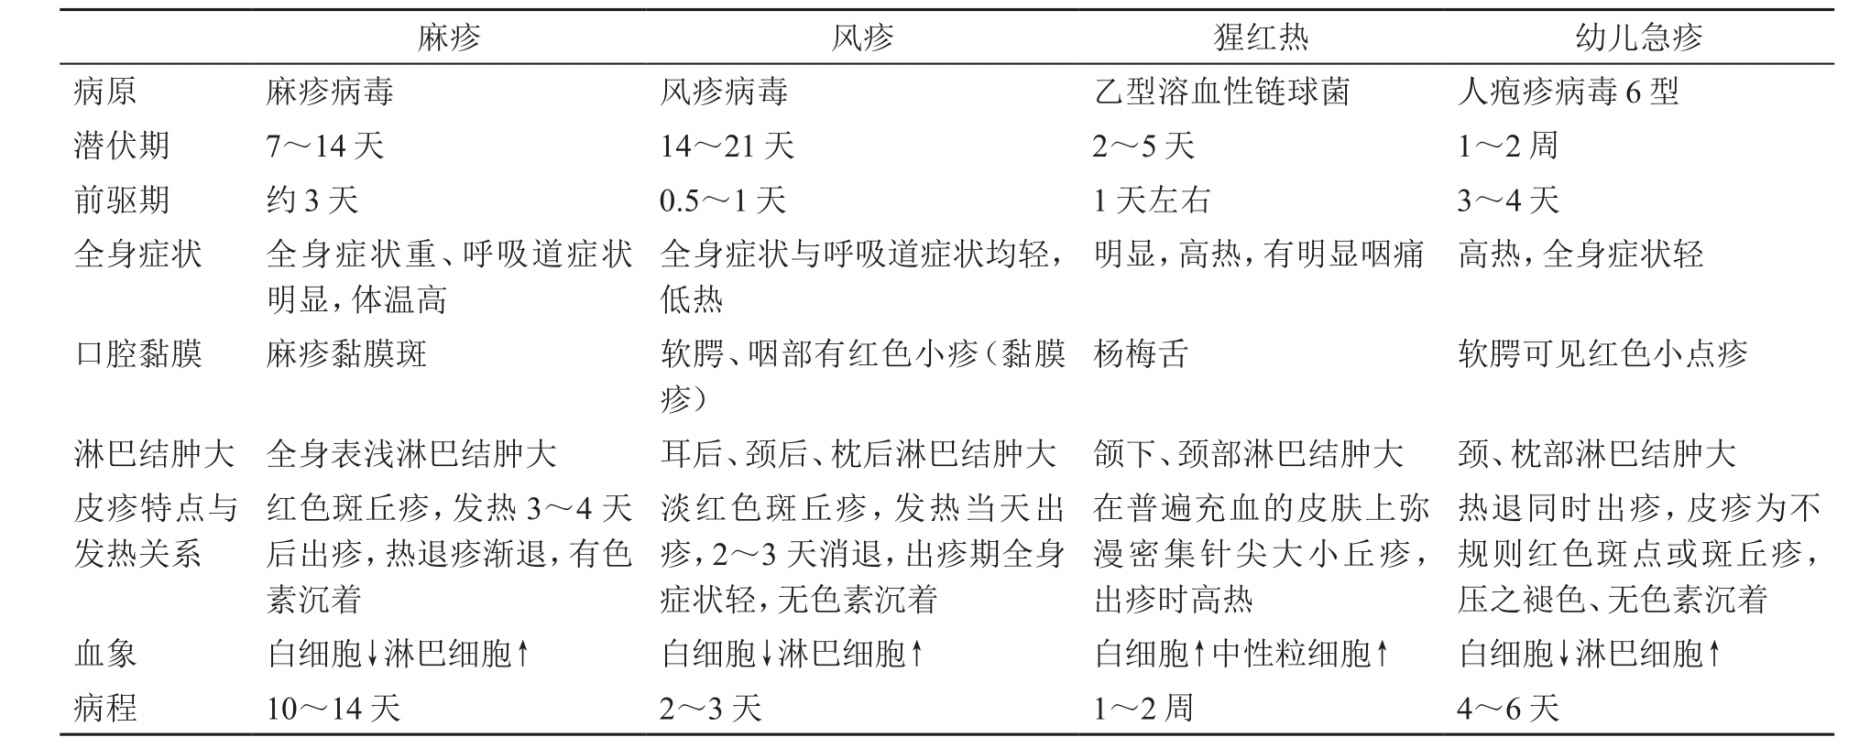
\includegraphics[width=6.79167in,height=2.71875in]{./images/Image00364.jpg}
\end{table}

祖国医学认为麻疹系热毒侵犯肺脾二经所致。治则为初热期(前驱期)应驱邪外出,宜辛凉透表,可用宣毒发表汤或升麻葛根汤加减,外用透疹药(生麻黄、芫荽子、西河柳、紫浮萍各15g)放入布袋中煮沸后在床旁蒸熏,或稍凉后以药汁擦面部、四肢,以助出疹。见形期(出疹期)宜清热解毒透疹,用清热透表汤或银翘解毒丸;热症重者可用三黄石膏汤或牛角地黄汤;虚弱肢冷者用人参败毒饮或补中益气汤。收没期(恢复期)宜养阴清热,可用沙参麦冬汤或竹叶石膏汤加减。

\subsubsection{治疗并发症}

\paragraph{肺炎}

按一般肺炎处理,继发细菌感染应选用1~2种抗菌药物治疗。高热中毒症状严重者,可考虑短期应用肾上腺皮质激素。吸氧,适当补液及支持疗法。

\paragraph{喉炎}

保持居室内一定湿度,保持患者安静,烦躁不安时及早用镇静剂,并给雾化吸入(每100ml雾化液中加氢化可的松100mg、麻黄碱1mg),每1~4小时1次。选用1~2种有效抗生素,重症者短期应用大剂量皮质激素静滴。喉梗阻进展迅速者,应及早考虑气管插管或行切开术。

\paragraph{心血管功能不全}

心力衰竭时给予强心、利尿、扩血管处理;周围循环衰竭时按感染性休克治疗。参见有关章节。

\paragraph{脑炎}

参考乙脑治疗,重点在对症处理。SSPE者可试用干扰素、转移因子等治疗,但疗效不确切。

\protect\hypertarget{text00218.html}{}{}

\hypertarget{text00218.htmlux5cux23CHP7-4-4}{}
参 考 文 献

1. 杨绍基,任红.传染病学.第7版.北京:人民卫生出版社,2008:69

2. 李梦东 ,王宇明.实用传染病学.第3版.北京:人民卫生出版社,2004:304

3. Tischer A,Andrews N,Kafatos G,et al. Standardization of
measles,mumps and rubella assays to enable comparisons of
seroprevalence data across 21 European countries and Australia.
Epidemiol Infect,2007,30:1-11

\protect\hypertarget{text00219.html}{}{}

\chapter{流行性乙型脑炎}

流行性乙型脑炎(epidemic encephalitis
B),亦称日本乙型脑炎,简称乙脑,是由乙脑病毒引起的、以脑实质炎症为主要病变的中枢神经系统(CNS)急性传染病。本病经蚊媒传播,多发生于夏秋季,患者一般以儿童较多。临床以发病急骤、高热、意识障碍、抽搐、呼吸衰竭、脑膜刺激征等为主要特征。病死率较高,达10\%左右,重症患者可留有后遗症。

\subsection{病因与发病机制}

乙脑病毒属披盖病毒科B组虫媒病毒,是一种RNA病毒。有包膜,RNA包被于单股多肽的核衣壳蛋白中组成病毒颗粒的核心。包膜中镶嵌有糖基化蛋白(E蛋白)和非糖基化蛋白(M蛋白),E蛋白是病毒的主要抗原成分,由它形成的表面抗原决定簇,具有血凝活性和中和活性,同时还与多种重要的生物学活性密切相关。乙脑病毒易被常用消毒剂所杀灭,不耐热,对低温和干燥抵抗力较强。乙脑病毒的抗原性稳定,较少变异。人与动物感染乙脑病毒后,可产生补体结合抗体、中和抗体及血凝抑制抗体,对这些特异性抗体的检测有助于临床诊断和流行病学调查。

乙脑是人畜共患的自然疫源性疾病,人与许多动物(如猪、牛、马、羊、鸡、鸭等)都可成为本病的传染源。人被乙脑病毒感染后,可出现短暂的病毒血症,但病毒数量少,且持续时间短,所以人不是本病的主要传染源。动物中的家畜、家禽和鸟类均可感染乙脑病毒,尤其是猪的感染率高,仔猪经过一个流行季节几乎100\%受到感染,感染后血中病毒数量多,病毒血症期长,加上猪的饲养面广,更新率快,因此猪是本病的主要传染源。

乙脑主要通过蚊虫叮咬而传播。库蚊、伊蚊和按蚊的某些种都能传播本病,而三带喙库蚊是主要传播媒介。当它们叮咬感染乙脑病毒的动物尤其是猪后,病毒进入蚊体内迅速繁殖,经叮咬将病毒传给人和动物。现已证实蚊感染后可带病毒越冬,病毒可经蚊卵传代,因此蚊是本病的最重要的传播媒介和长期储存宿主。人群对本病普遍易感,感染后多数呈隐性感染,乙脑患者与隐性感染者之比为1∶(300~2000)。病后多产生持久的免疫力,再次发病者极为少见。当人体被带病毒的蚊虫叮咬后,病毒进入人体,经淋巴管或毛细血管到达单核巨噬细胞系统,在单核吞噬细胞内繁殖,然后进入血液循环形成病毒血症,继而在全身非神经组织中繁殖,如不侵入CNS,则成隐性感染,并可获得对乙脑的免疫力。仅当机体免疫力低下和(或)病毒数量多、毒力强时,病毒可通过血脑屏障侵入CNS,引起广泛性病变,发生脑炎,称为显性发病。脑寄生虫、癫痫、高血压、脑血管病和脑外伤等可使血脑屏障功能降低,使病毒更易侵入CNS。

乙脑脑组织的损伤机制包括:①病毒对神经组织的直接侵袭:乙脑病毒是嗜神经病毒,易直接侵袭神经组织,细胞凋亡现象是乙脑病毒导致神经细胞死亡的普遍机制。②脂质过氧化损伤:在乙脑发病时,中枢神经组织中大量一氧化氮(NO)产生,诱发脑组织细胞脂质过氧化,导致损伤。③免疫损伤:当体液免疫诱导出的特异性IgM与病毒抗原结合后,就会沉积在脑实质和血管壁上,激活补体和细胞免疫,引起免疫攻击,导致血管壁破坏,附壁血栓形成,脑组织细胞供血障碍和死亡。

乙脑的病变范围较广,可累及整个CNS灰质,但以大脑皮层及基底核、视丘最为严重。其基本病变为神经细胞变性、坏死,形成软化灶;血管充血,周围淋巴细胞浸润与胶质细胞增生。部分病例出现小脑扁桃体疝或钩回疝。

\subsection{诊断}

\subsubsection{流行病学资料}

本病在热带地区全年均可发生,但在亚热带和温带地区有严格的季节性,好发于夏末秋初,80\%~90\%集中在7~9月,随各地气候流行高峰可提早或推迟1个月。10岁以下儿童多见,尤以2~6岁儿童发病率最高。儿童接种乙脑疫苗后发病减少,但成人发病有增加。当夏秋季节(7~9月),起病前3周内在流行地区有蚊虫叮咬史,尤其是儿童突然发热、头痛、呕吐、嗜睡或烦躁等现象,且在短期内逐渐加重而无明显上呼吸道炎症表现者,应首先考虑本病。

\subsubsection{临床表现特点}

乙脑病毒侵入人体约经4~21天(一般为10~14天)潜伏期后出现神经症状。按病程可分为以下四个时期:

\paragraph{初期}

为病初的1~3天。起病急,1~2天内体温升高达39℃,伴有头痛、恶心、呕吐、嗜睡、烦躁、结合膜及咽部充血。部分患者可有颈项强直及抽搐,但神志尚清楚。极重型患者本期经过甚短,于起病1~2天内就出现高热、频繁抽搐、深度昏迷而进入极期。

\paragraph{极期}

病程的第4~10天。患者除全身毒血症状加重外,突出表现为脑损害症状更为明显。主要表现有:

\hypertarget{text00219.htmlux5cux23CHP7-5-2-2-2-1}{}
(1) 高热:

为本病必有的表现。体温稽留于39~40℃以上,并持续不退直至极期结束,一般持续7~10天,重症者达3周以上。发热越高,热程越长,病情越重。

\hypertarget{text00219.htmlux5cux23CHP7-5-2-2-2-2}{}
(2) 意识障碍:

多发生于第3~8病日,轻者嗜睡,重者出现昏迷,成年患者偶有谵妄、定向力障碍、狂躁等。意识障碍通常持续1周左右,重者可长达1个月以上。

\hypertarget{text00219.htmlux5cux23CHP7-5-2-2-2-3}{}
(3) 抽搐或惊厥:

抽搐或惊厥发生率约40\%~60\%。由于脑部病变的部位与程度不同,可有轻度的手、足、面部的抽搐,以至出现肢体阵挛性或全身强直性抽搐。抽搐可因脑水肿、脑部广泛炎症、脑缺氧及高热等引起,是乙脑病情严重的表现,一般均伴有意识障碍,重者可伴有发绀和呼吸暂停。

\hypertarget{text00219.htmlux5cux23CHP7-5-2-2-2-4}{}
(4) 呼吸衰竭:

是本病最主要的死亡原因。中枢性呼吸衰竭可由大脑皮质、下丘脑、脑桥的病变抑制了延脑呼吸中枢的功能所致;或延脑呼吸中枢自身的炎症所致;也可由弥漫性脑水肿伴显著的颅内压增高、脑疝所引起。表现为呼吸表浅、节律不齐、叹息样呼吸、潮式呼吸、呼吸暂停、抽泣样呼吸及下颌呼吸等,最后呼吸停止。外周性呼吸衰竭主要因呼吸道痰阻、肺部感染或肺不张、脊髓病变所致膈肌或肋间肌麻痹等原因引起,表现为呼吸困难、发绀、呼吸减弱,但呼吸节律始终整齐。

\hypertarget{text00219.htmlux5cux23CHP7-5-2-2-2-5}{}
(5) 颅内压增高和脑膜刺激征:

本病多有不同程度的颅内压增高,较大儿童及成人均有不同程度的脑膜刺激征。重症患者可发生脑疝,以钩回疝(小脑幕切迹疝)较为多见,表现为昏迷突然加深,呼吸节律异常,疝侧瞳孔散大和上睑下垂,对侧肢体瘫痪和锥体束征阳性。

\hypertarget{text00219.htmlux5cux23CHP7-5-2-2-2-6}{}
(6) 其他神经系局灶症状:

由于本病常有广泛的中枢神经系损害,因而可出现各种神经反射异常和神经系体征。大脑锥体束受损可出现肢体痉挛性瘫痪、肌张力增强和病理征阳性。大脑半球损害表现为去大脑强直。下丘脑损害可出现体温调节障碍。如延脑受损可发生延髓性麻痹。前庭小脑受损害可有眼球震颤及瞳孔变化。自主神经受累可出现面赤、发热、偏侧出汗、大小便失禁、尿潴留、直肠麻痹等。乙脑的神经系症状常在病程第一周内达高峰,第二周后极少出现新的神经系症状。

\paragraph{恢复期}

极期(持续1周左右)过后,体温多在2~5天内降至正常。神经精神症状日渐好转,一般于2周左右完全恢复,部分患者恢复较慢需数月。恢复期可有低热、多汗、言语障碍、吞咽困难、肢体麻痹、不自主动作、抽搐发作、表情缺失等。少数患者有智能障碍或精神异常。

\paragraph{后遗症期}

发病半年后仍留有神经精神障碍者称为后遗症。约占5\%~20\%。以失语、瘫痪及精神失常最常见,重症病例可有肢体强直、角弓反张、不自主动作、视力障碍及痴呆等。

\subsubsection{临床分型}

根据临床表现及临床病程经过,可分为以下四型,其中轻型和普通型最多,占2/3。但病情可以从轻型发展成为严重类型。

\paragraph{轻型}

患者神志清楚,可有轻度嗜睡。体温38~39℃,仅在高热时才可能有抽搐。可有轻度脑膜刺激征。大多在一周左右恢复。

\paragraph{中型(普通型)}

体温39~40℃,有不同程度的意识障碍,脑膜刺激征明显,有轻度抽搐,病理反射阳性,浅反射减弱或消失,或有脑神经麻痹、运动障碍等。病程约7~14天左右,大多无恢复期症状。

\paragraph{重型}

神志不清,持续高热40℃以上,有反复或持续性抽搐,深反射先亢进后消失,浅反射消失,病理反射阳性。脑膜刺激征明显,肢体瘫痪或出现呼吸衰竭。病程多在2周以上,恢复期常有明显的神经精神症状,部分患者可有后遗症。

\paragraph{极重型(暴发型)}

起病急骤,体温迅速于病后1~2天内上升到40℃以上。深昏迷,反复或持续抽搐,迅速出现脑疝及中枢性呼吸衰竭。本型常于短期内(一般3天左右)出现呼吸循环衰竭而死亡,幸存者多有严重后遗症。此型占总数的5\%左右。

此外,尚有少数表现为脑干脑炎、脑膜脑炎、脊髓炎或不完全型等特殊临床类型。

\subsubsection{辅助检查}

\paragraph{血象}

血白细胞增多,常达(10~30)× 10\textsuperscript{9}
/L,中性粒细胞增多为主,并有核左移,嗜酸性粒细胞减少,这与一般病毒感染不同。部分患者血象始终正常。

\paragraph{脑脊液检查}

外观无色透明或微混,压力增高,白细胞数轻度增高,多在(50~500)×
10\textsuperscript{6} /L之间,个别患者可达1000 × 10\textsuperscript{6}
/L以上,起病后2~5天以中性粒细胞为主,以后则以淋巴细胞占多数。蛋白轻度增高,大多不超过1.0g/L,糖正常或稍高,氯化物正常。细菌检查阴性。极少数患者脑脊液常规与生化正常。

\paragraph{血清学检查}

乙脑的确诊有赖于血清学诊断。常用的试验有:

\hypertarget{text00219.htmlux5cux23CHP7-5-2-4-3-1}{}
(1) 补体结合试验:

补体结合抗体为IgG抗体,特异性高、灵敏度强,但出现较迟,阳性大多出现在4~7周,双份血清抗体效价4倍以上增高即为阳性。仅用于回顾性诊断和流行病学调查。

\hypertarget{text00219.htmlux5cux23CHP7-5-2-4-3-2}{}
(2) 血凝抑制试验:

此抗体于病后3~5天出现,第2周达高峰,可持续1年以上。阳性率达81\%左右,双份血清对照抗体效价增高4倍以上为阳性。由于乙脑病毒的血凝素抗原与同属病毒登革热病毒和黄热病病毒等有弱的交叉反应,故可出现假阳性。

\hypertarget{text00219.htmlux5cux23CHP7-5-2-4-3-3}{}
(3) 特异性IgM抗体测定:

特异性IgM抗体于感染后第4天即可出现,2~3周达到高峰,故单份血清即可作出早期诊断。常用酶联免疫吸附试验(ELISA)测定IgM抗体,于病后第4天即可呈阳性反应,一般病后2周阳性率可达70\%~90\%,具有较高的敏感性和特异性,可提高乙脑的早期诊断率,已被广泛采用。

\paragraph{病原学检查}

①病毒分离:对疑诊死亡病例取脑组织或延髓穿刺取脑组织,病毒分离阳性率较高,作为回顾性诊断。②病毒抗原或核酸检测:在组织、血液或其他体液中通过直接免疫荧光或PCR可检测到乙脑病毒抗原或特异性核酸。

\subsubsection{诊断注意事项}

根据流行季节(7~9月)发病,儿童及青少年,突然起病,有发热、头痛、呕吐、嗜睡、昏迷、抽搐、脑膜刺激征及神经系统症状体征,结合血及脑脊液(CSF)的检查,一般诊断不难。必要时可作上述血清学检查。但应注意与下述几种疾病相鉴别:

\paragraph{中毒型菌痢}

二者均多发生于夏秋季,儿童多见。但中毒型菌痢起病更急,发病1~2天内,突然出现发热、抽搐、昏迷和感染性休克,一般无脑膜刺激征。CSF无改变,肛拭子取粪便检查时可见大量脓细胞。镜检和粪便培养可明确诊断。

\paragraph{化脓性脑膜炎(化脑)}

化脑患者脑膜刺激征显著。CSF外观混浊,白细胞计数常在1000 ×
10\textsuperscript{6}
/L以上,中性粒细胞为主,蛋白质明显升高,糖降低。早期及未彻底治疗的化脑,CSF不易与乙脑区别,应反复进行血液及CSF细菌学检查,若阴性,可进一步作血清学检查。凡不能排除化脑者,应毫不迟疑地应用抗生素治疗。

\paragraph{脑型疟疾}

常有不规则发热及肝脾肿大,血中可查到疟原虫。CSF检查基本正常。

\paragraph{钩端螺旋体病脑膜脑炎型}

易与乙脑相混淆。但钩端螺旋体病多有疫水接触史,早期肌痛及腓肠肌压痛明显,眼结膜多充血,嗜睡多见,而昏迷抽搐者少,CSF改变轻。血清学检查可与乙脑相区别。

\paragraph{其他病毒性脑炎及脑膜炎}

较常见的有:①肠道病毒性脑膜脑炎:多由柯萨奇病毒和埃可病毒引起,多发生于夏秋季,CSF改变与乙脑相似,易误诊为乙脑。但其起病不如乙脑急骤,临床症状也较轻,多不发生呼吸衰竭,预后好,很少有后遗症。确诊依靠病毒分离及血清学检查。②单纯疱疹病毒性脑炎:由疱疹病毒Ⅰ型引起,病情重,病死率高达30\%左右。本病特殊定位在颞叶及额叶,故可出现脑局灶症状。可用CSF中病毒分离、CT及脑组织中HSV抗原检查确诊。③流行性腮腺炎脑膜脑炎:多发生于冬春季,一般发生于腮腺肿大后1周内,但也有发生于腮腺肿大之前或仅有脑膜脑炎而无腮腺肿大者。而乙脑也常见有腮腺肿大者,随病情好转腮腺肿大消退。但流行性腮腺炎脑膜炎一般病情较轻,腮腺肿大常伴有颌下腺、舌下腺及睾丸肿大。鉴别有赖于血清淀粉酶测定及血清学检查。

\subsection{附} 诊断标准

\paragraph{疑似病例}

在疾病流行地区的蚊虫叮咬季节,出现发热、头痛、恶心、呕吐、嗜睡、颈抵抗、抽搐等中枢神经系统症状。

\paragraph{确诊病例}

①曾在疫区有蚊虫叮咬史;②高热昏迷、肢体痉挛瘫痪、脑膜刺激症状、及大脑锥体束受损(肌张力增高、病理征阳性);③高热、昏迷、抽搐、狂躁,进而呼吸衰竭、循环衰竭而死亡;④从脑组织、脑脊液或血清中分离出乙型脑炎病毒;⑤CSF或血清中特异性IgM抗体阳性;⑥恢复期血清中特异性IgG抗体滴度比急性期有4倍以上升高者或急性期抗体阴性,恢复期血清抗体阳性。

临床诊断:疑似病例加①和②或①+②+③并除外细菌性脑膜脑炎。

实验确诊:疑似病例加④或⑤或⑥。

\subsection{治疗}

本病目前尚无特效的抗病毒治疗药物,早期可试用利巴韦林、干扰素等。宜密切观察病情变化,积极采取对症治疗和中西医结合治疗,正确处理高热、惊厥、控制脑水肿和呼吸衰竭等危重症状,预防并发症与继发感染。

\subsubsection{一般治疗及护理}

患者应隔离于有防蚊和降温设施的病房,室温控制在30℃以下。保持安静,避免刺激。定期观察患者的神志、体温、血压、呼吸、瞳孔及肌张力的变化。对昏迷者应定时翻身、拍背、吸痰,防止褥疮发生。不能进食者鼻饲,计出入水量,按生理需要补液,维持水、电解质平衡。成人每日输液量为1500~2000ml,儿童每天50~80ml/kg为宜。

\subsubsection{对症处理}

高热、抽搐及呼吸衰竭是危及乙脑患者生命的三大主征,可互为因果,形成恶性循环。高热增加耗氧量,加重脑水肿和神经细胞病变,使抽搐加重;抽搐又加重缺氧,导致呼吸衰竭并进一步加重脑组织病变,使体温升高。因此,及时控制高热、抽搐及呼吸衰竭是抢救乙脑患者的关键。治疗应着重于以下方面:

\paragraph{降温}

应采取综合性降温措施(物理降温为主,药物降温为辅),使患者肛温控制在38℃左右。①物理降温:如头部用冰帽连续降温,颈部、腋下及腹股沟部置冰袋,30\%~50\%酒精擦浴、冷盐水灌肠等。同时使室温降至25℃以下。②药物降温:为配合物理降温,可应用小剂量退热药物,如吲哚美辛(消炎痛)口服或鼻饲,每次12.5~25mg,每4~6小时1次;对暂时不能口服或鼻饲者,可采用吲哚美辛栓剂,肛内置留。幼儿、年老体弱者可用10\%~20\%安乃近滴鼻。应防止用药过量致大量出汗而引起循环衰竭。严重者给予氢化可的松100~300mg/d或地塞米松5~10mg/d。③亚冬眠疗法:持续高热、反复惊厥的患者可采用亚冬眠疗法。常用氯丙嗪和异丙嗪,每次各0.5~1mg/kg,每4~6小时肌内注射1次。使肛温维持在38℃左右,维持较长时间,在度过疾病极期后,逐渐撤除亚冬眠,一般为3~5天。但应注意冬眠疗法有抑制呼吸中枢及咳嗽反射,使呼吸道分泌物聚集等缺点,使用时要权衡利弊。

\paragraph{控制抽搐}

引起惊厥的原因有高热、颅内压增高、脑实质炎症、痰阻缺氧、低血钙及低血钠性脑病等。应首先针对不同原因采取相应措施,如因呼吸道痰液阻塞造成脑缺氧及脑水肿所致惊厥者,应以及时吸痰、吸氧为主;低血钠性脑病及低血钙引起的惊厥应及时纠正电解质紊乱及代谢性酸中毒。如惊厥的原因为脑实质炎症,则应及时给予镇静剂,常用的药物有:①地西泮:成人用量为每次10~20mg,儿童每次0.1~0.3mg/kg(不超过10mg),肌内注射或缓慢静脉注射。②水合氯醛:成人每次1.5~2.0g,儿童每次60~80mg/kg(每次不超过1.0g),稀释后鼻饲或保留灌肠。③异戊巴比妥钠:成人每次0.2~0.5g,儿童每次5~10mg/kg,溶入5\%~10\%葡萄糖液20ml中,缓慢静脉注射(>
5分钟)。本药适用于其他止痉药不易控制的抽搐。因该药有明显的呼吸抑制作用,故用药过程中如呼吸减慢或惊厥停止,应立即终止注射。④苯巴比妥钠:成人每次0.1~0.2g,儿童每次5~8mg/kg,肌内注射。

\paragraph{脱水}

颅内压增高是呼吸衰竭、抽搐及脑疝的根本原因,需做积极处理。常用的脱水剂有20\%甘露醇、利尿剂、高渗葡萄糖等,详见第41章“颅高压危象”的治疗部分。肾上腺皮质激素具有减轻炎症反应、改善脑水肿、减轻中毒症状和降温作用,但它可促使感染加重和扩散,仅主张短期用于重型和极重型患者。

\paragraph{呼吸衰竭的处理}

应根据引起呼吸衰竭的不同原因采取相应的措施。①保持呼吸道通畅,定时翻身并拍打胸背、吸痰及雾化吸入,对于有严重排痰障碍者可用纤维支气管镜吸痰。病情危重者,宜早行气管插管或气管切开建立人工气道。有下列指征时应尽早行气管切开:深昏迷,痰液阻塞,咳嗽反射消失,吞咽功能障碍,经处理无效者;脑干型脑炎,咽喉部分泌物聚集,病情进展者;延脑麻痹或假性延脑麻痹,或呼吸肌麻痹,经吸痰给氧仍不能维持换气功能者;老年人呼吸衰竭、排痰困难,或乙脑极期合并肺炎、肺不张,发绀进行性加重者。②氧疗,可选用鼻导管或面罩给氧。③脱水降颅内压治疗。④中枢性呼吸衰竭时可应用呼吸兴奋剂,可选用洛贝林(成人每次3~6mg,儿童每次0.15~0.2mg/kg)、尼可刹米(成人每次0.375~0.75g,儿童每次5~10mg/kg)等肌注或静脉滴注。⑤改善脑微循环:使用血管扩张药可改善脑微循环、减轻脑水肿、解除脑血管痉挛和兴奋呼吸中枢。常用东莨菪碱,成人0.3~0.5mg/次,儿童每次0.02~0.03mg/kg;或山莨菪碱成人每次20mg,儿童每次0.5~1mg/kg,以5\%葡萄糖液稀释后,每隔10~30分钟静脉缓注1次,直至呼吸循环改善为止,一般用1~5天。此外,纳洛酮对退热、止痉、神志转清、纠正呼衰等有较好作用,可早期应用。

\subsubsection{中医中药治疗}

基本上按温病辨证施治,多采用清热解毒、芳香化湿相结合方法,依卫气营血分型立分。常选用银翘散、白虎汤、黄连解毒汤、清营汤等方剂加减,可配合应用紫雪丹、至宝丹、安宫牛黄丸等。亦可配合选用一些中药注射制剂,如板蓝根注射液、醒脑静注射液等,其中醒脑静注射液使用方便,既可肌内注射,也可静脉应用,具有降温、止惊、降颅内压、促苏醒等作用,可作为首选的中药注射制剂之一。

\subsubsection{其他治疗}

病初可用广谱抗病毒药物如利巴韦林静脉滴注。α干扰素有增强机体细胞抗病毒的能力,但其有效程度尚待进一步明确。实验研究证实,乙脑病毒单克隆抗体能迅速中和游离病毒,消除病毒血症,抑制病毒繁殖,控制中枢神经系统病变的发展。

\subsubsection{恢复期及后遗症的处理}

加强营养,细心护理,防止褥疮、肺炎等并发症。肢体瘫痪者应保持肢体功能位,防止肢体畸形发生。对病情稳定、无抽搐的瘫痪、失语患者可采用高压氧治疗。恢复期可用针灸、理疗、推拿、功能锻炼等综合措施,并给予改善神经细胞功能的药物。

\protect\hypertarget{text00220.html}{}{}

\hypertarget{text00220.htmlux5cux23CHP7-5-5}{}
参 考 文 献

1. 李梦东 ,王宇明.实用传染病学.第3版.北京:人民卫生出版社,2004:459

2. 杨绍基,任红.传染病学.第7版.北京:人民卫生出版社,2008:92

3.
赵川,向光明,余光开.流行性乙型脑炎的研究进展.医学综述,2005,11(12):1119

\protect\hypertarget{text00221.html}{}{}

\chapter{狂 犬 病}

狂犬病(rabies)是由狂犬病毒(rabies
virus)引起的一种侵犯中枢神经系统为主的急性人兽共患传染病,因常有恐水的临床表现,故又称恐水症(hydrophobia)。临床表现为特有的恐水、怕风、恐惧不安、发作性咽肌痉挛、进行性瘫痪等,病死率高达100\%,一般在发病后3~6天内死于循环或呼吸衰竭。

\subsection{病因与发病机制}

本病的病原为狂犬病毒,属单股RNA病毒。病毒形似子弹,大小约75nm ×
180nm。狂犬病毒含5个结构基因,即G、N、L、P和M基因,分别编码糖蛋白、核蛋白、转录酶大蛋白、磷蛋白和基质蛋白。糖蛋白能与Ach受体结合,决定了狂犬病毒的嗜神经性,能刺激机体产生保护性免疫反应。核蛋白是荧光免疫法检测的靶抗原,有助于临床诊断。病毒对外界抵抗力不强,易被大多数有机溶剂、氧化剂及表面活性物质(苯扎溴铵、肥皂、去垢剂)灭活。带狂犬病毒的动物是本病的传染源,在我国病犬是主要的传染源,人狂犬病由病犬传播者占80\%~90\%,其次为猫、猪、牛、马等家畜。蝙蝠、浣熊、臭鼬、狼、狐狸等野生动物是发达国家和基本上控制了犬的狂犬病地区的主要传染源。人患病后唾液含有少量病毒,有可能成为传染源,但尚待证实。病毒主要通过咬伤传播,也可由带病毒动物的唾液,经各种伤口和抓伤、舔伤的黏膜和皮肤入侵,少数可在宰杀病犬、剥皮、切割等过程中被感染。人群对本病普遍易感,兽医与动物饲养员尤其易感。未作预防注射者被病犬咬伤后的平均发病率为15\%~20\%,病狼咬伤者为50\%~60\%。被病兽咬伤后是否发病与下列因素有关:①咬伤部位:头面部、颈部、手部被咬伤后发病机会多;②咬伤的严重程度:伤口深而大者发病机会多;③局部处理情况:咬伤后迅速彻底进行伤口处理者发病机会少;④及时、全程、足量注射狂犬疫苗和免疫球蛋白者发病率低于1\%,国内报告为0.15\%;⑤被咬伤者免疫功能低下或免疫缺陷者发病机会多。本病主要分布在城镇、农村和边远山区。人狂犬病发病之前,常有犬狂犬病流行。

病毒对神经组织有强大的亲和力。实验证明,在潜伏期和发病期间并无病毒血症。狂犬病的发病过程可分为3个阶段:①局部组织内病毒小量繁殖期:人被感染动物咬伤后病毒自咬伤部位侵入,先在入侵处的横纹肌细胞内缓慢增殖,侵入附近的神经末梢,选择性地在神经肌肉接合部与乙酰胆碱受体结合而进入周围神经组织。此期一般在3~5天之内,也有报道达1~2周之久。②侵入中枢神经期:病毒沿周围神经的轴索浆向中枢神经作向心性扩展,其速度约每小时3mm。到达脊髓的背根神经节后,病毒即在其内大量繁殖,然后侵入脊髓和整个中枢神经系统,主要侵犯脑干和小脑等处的神经元。③向器官扩散期:病毒自中枢神经系统向周围神经离心性扩散,侵入唾液腺、肾上腺、肾、肺、肝、骨骼肌、心脏等各器官组织,尤以唾液腺、舌部味蕾、嗅神经上皮等处病毒量多。由于迷走神经核、吞咽神经核及舌下神经核受损,而发生吞咽肌及呼吸肌痉挛,临床上出现恐水、呼吸困难、吞咽困难等表现;交感神经兴奋,使唾液分泌和出汗增多;交感神经、迷走神经和心脏神经节受损时可产生心血管功能紊乱和猝死。

病理变化主要为急性弥漫性脑脊髓炎,以大脑基底面海马回、脑干部位及小脑损害最明显。具有特征性的病变是嗜酸性包涵体,称内基小体(Negri
body),为狂犬病毒的集落,最常见于海马及小脑普肯耶细胞中。

\subsection{诊断}

\subsubsection{病史}

发病前有被犬、猫等患病动物咬伤史,有皮肤黏膜破损处被其唾液污染或接触兽、畜皮,进食兽、畜肉史。

\subsubsection{临床表现特点}

本病潜伏期长短不一,最短可至4天内,最长可达数十年之久,通常为1~3个月。短潜伏期常见于头面部、颈部咬伤以及严重或多部位咬伤者。典型的临床经过可分为三期,即前驱期、兴奋期和麻痹期(瘫痪期)。

\paragraph{前驱期(侵袭期)}

在兴奋状态出现前,多数患者有低热、头痛、周身不适、倦怠、纳差、恶心、腹痛腹泻等症状,同时伴有或随后出现焦虑、抑郁、幻觉、失眠、注意力不集中、恐慌不安,对声、光、风、痛等刺激比较敏感,并有喉头紧缩感。具有诊断意义的早期症状是在愈合的伤口及其神经支配区有痒、痛、麻及蚁走等异样感觉,约发生于80\%的病例。患者可表现有受伤处出现烧灼或针刺样疼痛、麻木感、冷感或蚁行感,或在伤口的瘢痕处发痒(此乃病毒繁殖时刺激神经元所致),可波及整个躯体甚至全身发痒,由此可引起剧烈的搔抓使多处皮肤受伤,这些症状高度提示狂犬病的可能。本期持续2~4天。

\paragraph{兴奋期(激动期)}

患者逐渐进入高度兴奋状态,突出表现为恐怖不安、恐水怕风、发作性咽喉肌痉挛,呼吸困难、排尿排便困难、高热、多汗、流涎等。恐水为本病所特有,当饮水、见水、闻及流水声或仅仅提及饮水时,均可引起反射性咽喉肌痉挛,患者极度的痛苦和恐惧,患者虽渴而不敢饮,饮后也无法下咽,从而引起脱水。80\%的患者有此典型表现。有些患者感觉咽喉部疼痛和阻塞,促使用双手拉扯自己的咽喉部。畏风也是本病的常见症状。对外界各种刺激如轻微的风、光、声音或触摸等均可引起咽喉肌和呼吸肌痉挛,由于声带痉挛导致说话不清,甚至失音。交感神经常常亢进,表现为体温和血压升高,心率增快,唾液分泌增加,大汗淋漓,瞳孔散大,对光反射迟钝等。部分患者出现下丘脑和杏仁核功能异常,可导致性欲增强,或为嗜色狂或慕男狂,男性患者在一日内可试图多次性交或自发性射精。多数患者神志清楚,表情痛苦焦急,狂躁不安;随着兴奋状态的增长,部分患者可出现精神失常、谵妄、幻想幻视、强行挣扎,并试图逃出室外,也可能攻击或咬伤他人。病程进展迅速,大多在发作中死于呼吸、循环衰竭。本期持续1~3天。

\paragraph{麻痹期(瘫痪期)}

患者渐趋安静,痉挛发作停止,出现各种瘫痪,尤以肢体软瘫最为多见,也可表现为眼肌、颜面肌和咀嚼肌的瘫痪以及感觉减退、失音和反射消失等。本期中患者的呼吸逐渐微弱或不规则,可迅速因呼吸、循环衰竭而死亡。临终前多进入昏迷状态。本期持续6~18小时。

本病的整个病程一般不超过6天,超过10天者极少。除上述典型者外,有所谓“麻痹型”者,此型常见于吸血蝙蝠咬伤、受固定株病毒感染、接受角膜移植及儿童患者,约占狂犬病的2\%~20\%。其病理损害以脊髓、延脑为主,因咽喉肌麻痹不能说话,又称“哑型”狂犬病(dumb
rabies)。不同的是无兴奋期表现,前驱期后出现四肢麻木,麻痹从下肢开始,逐渐发展至全身麻痹,多无吞咽困难和恐水表现,也没有痉挛发作,神志始终清楚,终因衰竭而死亡,病程10天左右。

\subsubsection{辅助检查}

\paragraph{血象}

白细胞总数轻~中度升高,脱水时可达30 × 10\textsuperscript{9}
/L,以中性粒细胞为主。

\paragraph{脑脊液检查}

压力正常或稍高,细胞数稍高,以淋巴细胞为主,蛋白含量增多,糖及氯化物大致正常。

\paragraph{病原学检查}

\hypertarget{text00221.htmlux5cux23CHP7-6-2-3-3-1}{}
(1) 抗原检查:

可取患者的CSF或唾液直接涂片、角膜印片或咬伤部位皮肤组织或脑组织通过免疫荧光抗体法检测病毒抗原,阳性率可达98\%。此外,还可使用快速狂犬病ELISA检测病毒抗原。

\hypertarget{text00221.htmlux5cux23CHP7-6-2-3-3-2}{}
(2) 病毒分离:

取患者的唾液、脑脊液、皮肤或脑组织进行细胞培养或用乳小白鼠接种法分离病毒。

\hypertarget{text00221.htmlux5cux23CHP7-6-2-3-3-3}{}
(3) 内基小体检查:

于死后进行。取脑组织切片染色检查内基小体,阳性率70\%~80\%。

\hypertarget{text00221.htmlux5cux23CHP7-6-2-3-3-4}{}
(4) 核酸检测:

采用RT-PCR法检测狂犬病毒RNA。

\paragraph{抗体检查}

存活一周以上者做血清中和试验或补体结合试验检测抗体,效价上升者有诊断意义。此外,中和抗体还是评价疫苗免疫力的指标。

\subsubsection{诊断注意事项}

根据有狂犬动物咬伤或抓伤史,出现典型症状,即可作出临床诊断。确诊有赖于病原学检查。在病程早期或症状不典型的患者易被误诊,须与下述疾病鉴别:

\paragraph{破伤风}

有外伤史,潜伏期较短,主要是肌肉阵发性痉挛,且有牙关紧闭、角弓反张、苦笑面容等特点,但无狂躁、流涎、恐水、畏风等表现。

\paragraph{脊髓灰质炎}

多见于儿童,病程早期常有发热、头痛、出汗、兴奋、感觉过敏,出现肢体瘫痪后以上症状消失。脑脊液异常改变多见。

\paragraph{其他病毒性脑炎}

其他各型脑炎患者常出现高热、抽搐,但无流涎、恐水表现,且常有不同程度的意识障碍。狂犬病患者神志清楚。免疫学检查、病毒分离和临床转归等有助于鉴别。

\paragraph{狂犬病恐惧症(rabies phobia)}

癔症患者在被动物咬伤后几小时或1~2天出现咽喉部紧缩感、恐怖感,甚至出现恐水。这种假性恐水是一种夸张的动作,不能产生病理性反应,患者不出现发热、畏风、流涎,经暗示说服或对症治疗后可顺利恢复。

\paragraph{震颤性谵妄(delirium tremens)}

长期酗酒者,即使24小时未饮酒也能产生严重戒断状态。患者一般先因头部损伤或急性感染以及戒酒,表现有焦虑、震颤、出汗、谵妄,呈现动物或昆虫的逼真吓人的视幻觉或感觉性幻觉。谵妄和幻觉是本病的早期症状,却是狂犬病中的晚期表现。

\paragraph{狂犬病疫苗引起的神经系统并发症}

接种狂犬病疫苗后(多发生在首剂疫苗后2周)有时可出现发热、关节酸痛、肢体麻木、运动失调和各种瘫痪等症状,在应用疫苗过程中逐渐加重。与本病的“麻痹型”有时不易区别。但前者经停止接种,用激素治疗后大多数可恢复;死亡病例则须经内基小体和免疫学试验才能鉴别。

\subsection{治疗与预防}

本病无特异性治疗,病死率达100\%,故强调在咬伤后及时预防性治疗以防止发病。若已发病则采取对症治疗,尽量延长患者生存时间。

\subsubsection{发病时的处理}

仅能作对症处理:①首先将患者隔离在安静、光线较暗的单人房间,避免各种声、光、风等刺激,精心护理。医护人员最好进行狂犬病疫苗注射,接触患者应戴口罩、手套,以防患者唾液中的病毒污染皮肤及黏膜破损处。②应用镇静剂如氯丙嗪、苯巴比妥钠、地西泮(安定)等控制患者的兴奋状态。③鼻饲或静脉输液,补充血容量,纠正水电解质及酸碱平衡失调。④采取有效措施,维持患者心肺功能。必要时可作气管切开术,并应用肌肉松弛剂和间歇正压通气等。

\subsubsection{预防}

\paragraph{控制和管理传染源}

捕杀野犬,对饲养犬进行登记并做好预防接种。发现病犬、病猫应立即击毙,死后焚毁或深埋,严禁制皮和食用。咬过人的家犬、家猫应设法捕获,隔离观察10天以明确是否患病。仍存活的动物可暂时解除隔离,尽可能检查唾液是否带毒,以明确是否为“健康”带毒犬。

\paragraph{切断传播途径}

有狂犬病发生的地区,严禁饲养狗、猫等动物。狂犬病患者分泌物及被污染的环境应彻底消毒。

\paragraph{保护易感人群}

\hypertarget{text00221.htmlux5cux23CHP7-6-3-2-3-1}{}
(1) 暴露前狂犬病疫苗预防接种:

狂犬病高暴露风险者应当进行暴露前免疫,包括从事狂犬病研究的实验室工作人员、接触狂犬病患者的人员、兽医、山洞探险者等。接种3次,于0(注射当天)、7、21(或28)天各肌注1剂量(2ml)狂犬病疫苗。1年后加强1针次,以后每隔3~5年加强1针次。

\hypertarget{text00221.htmlux5cux23CHP7-6-3-2-3-2}{}
(2) 暴露后狂犬病疫苗预防接种:

如不慎被狗、猫或患病动物咬伤,或皮肤破损处被患病动物(狂犬、患者)唾液沾污者,应及早进行暴露后预防接种。一般于0、3、7、14、28天各肌注1剂量(2ml)狂犬病疫苗;如严重咬伤,可全程注射10针,于当天至第6天每天1针,随后于10、14、30、90天各注射1针。狂犬病疫苗不分体重和年龄,每针次均接种1个剂量(2ml)。接种狂犬病疫苗应当按时完成全程免疫,当某一针次出现延迟1天或者数天注射,其后续针次接种时间按延迟后的原免疫程序间隔时间相应顺延。对一种疫苗过敏者,可更换另一种疫苗继续原有免疫程序。

疫苗接种注射部位:上臂三角肌肌内注射。2岁以下婴幼儿可在大腿前外侧肌肉内注射,禁止臀部注射。

一般情况下,全程接种狂犬病疫苗后体内抗体水平可维持至少1年。如再次暴露发生在免疫接种过程中,则继续按照原有程序完成全程接种,不需加大剂量;全程免疫后半年内再次暴露者一般不需要再次免疫;全程免疫后半年到1年内再次暴露者,应当于0、3天各接种1针疫苗;在1~3年内再次暴露者,应当于0、3、7天各接种1针疫苗;超过3年者应当全程接种狂犬病疫苗。

\hypertarget{text00221.htmlux5cux23CHP7-6-3-2-3-3}{}
(3) 暴露后伤口处理:

伤口处理包括伤口彻底冲洗和消毒处理。伤口处理时间越早越好,就诊时如伤口已结痂或者愈合,则不主张进行伤口处理。伤口冲洗:用20\%肥皂水(或者其他弱碱性清洁剂)和一定压力的流动清水交替彻底冲洗,冲洗所有咬伤和抓伤处至少15分钟。然后用生理盐水(也可用清水代替)将伤口洗净,最后用无菌脱脂棉将伤口处残留液吸尽,避免在伤口处残留肥皂水或者清洁剂。深部伤口应用注射器插入伤口进行液体灌输、冲洗。如因疼痛,可给局部麻醉。消毒处理:伤口彻底冲洗后用2.5\%~3\%碘酒(聚维酮碘)或75\%酒精涂擦伤口。如伤口情况允许,应当尽量避免缝合或包扎。伤口轻微时,可不缝合,也可不包扎,可用透气性敷料覆盖创面。若有必要应在局部伤口处理后应用抗生素及破伤风抗毒素(TAT)等。对严重受染者(如头面部或颈部受伤,多处或深部受伤),确需缝合的,在完成清创消毒后,先用抗狂犬病血清(anti
rabies serum,ARS)或狂犬病免疫球蛋白(human rabies
immunoglobulin,HRIG)作伤口周围的浸润注射,使抗体浸润到组织中,以中和病毒,2小时后再行缝合和包扎;伤口深而大者放置引流条,以利于伤口污染物及分泌物的排出。伤口较深、污染严重者需应用抗生素及TAT等。

\hypertarget{text00221.htmlux5cux23CHP7-6-3-2-3-4}{}
(4) 被动免疫制剂的应用:

常用的有HRIG和ARS,以HRIG为佳,唯价格贵。HRIG用量为20U/kg,不需作皮肤过敏试验;ARS用量为40U/kg,用前需作皮肤过敏试验,即使阳性反应不能视为禁忌证,可在准备预防措施下进行脱敏注射。均应一次性足量注射。应当将被动免疫制剂全部浸润注射到伤口周围,所有伤口均应行浸润注射。当全部伤口进行浸润注射后尚有剩余被动免疫制剂时,应当将其注射到远离疫苗注射部位的肌肉。暴露部位位于头面部、上肢及胸部以上躯干时,剩余被动免疫制剂可注射在暴露部位同侧背部肌肉群(如斜方肌),狂犬病疫苗接种于对侧。暴露部位位于下肢及胸部以下躯干时,剩余被动免疫制剂可注射在暴露部位同侧大腿外侧肌群。如未能在接种狂犬病疫苗的当天使用被动免疫制剂,接种首针狂犬病疫苗7天内仍可注射被动免疫制剂。不能把被动免疫制剂和狂犬病疫苗注射在同一部位;禁止用同一注射器注射被动免疫制剂和狂犬病疫苗。

\protect\hypertarget{text00222.html}{}{}

\hypertarget{text00222.htmlux5cux23CHP7-6-4}{}
参 考 文 献

1. 张文武.急诊内科手册.北京:人民卫生出版社,2009:230

2. 杨绍基,任红.传染病学.第7版.北京:人民卫生出版社,2008:109

3. 中华人民共和国卫生部 .狂犬病暴露预防处置工作规范(2009年版).2009

\protect\hypertarget{text00223.html}{}{}

\chapter{肾综合征出血热}

肾综合征出血热(hemorrhagic fever with renal
syndrome,HFRS)又称流行性出血热(epidemic hemorrhagic
fever,EHF),是由汉坦病毒(Hanta
virus,HV)引起的,以鼠类为主要传染源的一种自然疫源性疾病。本病的主要病理变化是全身小血管和毛细血管的广泛性损害,以发热、低血压休克、充血出血及肾损害为主要临床特征。典型病例病程呈五期经过。

\subsection{病因与发病机制}

\subsubsection{病因}

汉坦病毒呈圆形、卵圆形或长形,直径70~210nm,有囊膜,囊膜上有突起。由于抗原结构的不同,HV至少有20个以上血清型。血清Ⅰ型病毒即汉滩病毒(Hantaan
virus,HTNV),又称野鼠型病毒或姬鼠型病毒,主要宿主动物是姬鼠;Ⅱ型病毒即汉城病毒(Seoul
virus,SEOV),又称家鼠型病毒,主要宿主动物是褐家鼠;Ⅲ型病毒即普马拉病毒(Puumala
virus,PUUV),又称鼠型病毒,主要宿主动物是欧洲棕背鼠;Ⅳ型病毒即希望山病毒(Prospect
Hill
Virus,PHV),又称为田鼠病毒,主要宿主动物是美国田鼠。我国主要流行的为Ⅰ型和Ⅱ型病毒。不同血清型的病毒,临床表现轻重程度也不一致。如Ⅰ型病毒常引起重型,Ⅱ型病毒常引起中型,Ⅲ型病毒引起轻型。目前认为Ⅰ型病毒感染者重于Ⅱ型病毒感染者,这可能与病毒的毒力有关,分子流行病学研究认为:汉滩病毒的变异速率较慢,但有时可有很微小的变化(几个甚至1个氨基酸的变化),这都有可能引起病毒毒力即致病性的巨大变化。汉坦病毒不耐热、不耐酸,高于37℃及pH
5.0以下易被灭活,56℃ 30分钟或100℃
1分钟可被灭活。对紫外线、乙醚、三氯甲烷(氯仿)和碘酒等敏感。

本病一年四季均可发病,但有季节性流行,且流行季节有双峰(春、夏季有一小峰,秋、冬季有一流行高峰)和单峰(只有秋、冬季一个高峰)两种类型。鼠类是肾综合征出血热的主要传染源。我国农村的主要传染源是黑线姬鼠和褐家鼠,城市的主要传染源是褐家鼠,实验动物的主要传染源是大白鼠。人类主要是通过接触受感染的动物的排泄物或分泌物而感染,尤其是经呼吸道传播,目前认为该途径是本病的主要传播途径。HFRS的流行,取决于主要宿主动物种群数量和带病毒率情况,同时与易感人群的免疫状态和接触汉坦病毒机会也有密切关系。人群对汉坦病毒普遍易感,但以青壮年、农民多见,儿童发病罕见。感染后抗体出现早,发热1~2天即可检测出IgM抗体,第7~10天达高峰;第2~3天可检测出IgG抗体,发病后第14~20天血清抗体可达高峰,持续时间较长。感染Ⅰ型病毒后,IgG抗体在体内可维持30多年,感染Ⅱ型病毒后,中和抗体只可维持2年;Ⅰ型病毒感染者对Ⅱ型病毒有一定的交叉免疫力,Ⅱ型病毒感染者对Ⅰ型病毒免疫力不强。HFRS病后可获持久免疫力,一般不发生再次感染发病,但隐性感染产生的免疫力多不能持久。随着我国经济的发展和农村经济模式的改变,目前家鼠型疫情逐年增多,野鼠型则相对减少,疫区逐渐由野鼠型、家鼠型趋向混合型。流行有一定的地区性,并可扩展而产生新疫区,多呈散发。在人口密集,带毒鼠数量多,人鼠接触机会较大的时候,会出现HFRS的暴发流行。洪涝灾害时,人群集居堤坝、高地,鼠类也向高处聚集逃避水患,造成人、鼠密度的同步增加,人鼠接触机会增多,可能引起HFRS的暴发。

\subsubsection{发病机制}

HFRS的发病机制迄今仍未完全阐明。近年来研究提示汉坦病毒感染为本病发病的始动因素,直接导致病毒感染脏器的组织细胞结构和功能的损害;同时又激发机体的免疫反应,释放并激活多种细胞因子、炎性介质而产生免疫病理损害,从而导致一系列复杂的病理生理过程,产生发热、低血压休克、出血和肾功能衰竭等临床经过。目前认为有如下机制:

\hypertarget{text00223.htmlux5cux23CHP7-7-1-2-1}{}
(一) 病毒直接致病作用(病毒学说)

主要依据是:①患者早期有病毒血症的相应症状如高热、寒战、乏力、全身酸痛等。②机体对不同血清型病毒的易感性不同,导致不同血清型的病毒所引起的临床症状严重程度也不同,但病情的轻重与病毒抗原差异及其毒力强弱有关。③病毒对人类呈泛嗜性感染,在心脏、肺、肝、肾、骨髓、胸腺、脾、淋巴结、血管内皮细胞、中枢神经系统、脊髓、外周血单核细胞等脏器、组织中均能检测到病毒抗原并分离出病毒,且病毒抗原分布多的脏器病理损害较重,提示脏器组织病变严重程度与病毒分布的数量有关。④体外培养正常人的血管内皮细胞、肝细胞、肾小管上皮细胞及骨髓细胞,并用病毒攻击后,均可出现细胞膜和细胞器损伤,表明在无免疫因素参与下,病毒具有直接引起病理损害作用。临床观察证明,肾综合征出血热的早期,患者已有微血管、肾脏的损害、血小板下降,称为原发性损伤,进一步提示病毒具有直接致病作用。为了进一步研究汉坦病毒的直接损害机制,对汉坦病毒结构蛋白的致病作用进行了深入的研究,结果提示在肾综合征出血热发病早期,汉坦病毒膜蛋白(MP)和核蛋白(NP)抗原均已出现,且其强度与病情及肾损害关系密切。通过对单核细胞的病毒结构蛋白与病情之间的动态观察,发现MP感染强度与尿素氮呈正相关,MP和NP抗原持续性高强度感染者预后较差,反之预后较好,且认为MP使细胞融合与脱落而直接致病。另外研究还发现MP与NP在发病初期阳性率最高,表达较强,早期应用抗病毒药物干扰素治疗后可使MP的滴度迅速下降,这为汉坦病毒具有直接致病作用提供了进一步的证据,为临床早期抗病毒治疗提供了理论依据。

\hypertarget{text00223.htmlux5cux23CHP7-7-1-2-2}{}
(二) 免疫发病机制(免疫学说)

主要依据是:①患者早期血液中特异性IgE和组胺均明显增高,嗜碱性粒细胞脱颗粒试验呈阳性反应,提示Ⅰ型变态反应参与发病过程。组胺增加可引起毛细血管扩张和血管通透性增加,产生皮肤、黏膜充血及水肿等。②患者早期血清补体下降,血中存在特异性循环免疫复合物,免疫组化提示抗原为病毒抗原,血清中也可检出抗基底膜和抗心肌抗体。在镜下可观察到皮肤小血管、毛细血管、肾小球、肾小管基底膜、血小板、红细胞表面、内皮细胞内及表面等均有特异性免疫复合物沉积,并可发现补体裂解片段,表明Ⅲ型变态反应参与发病过程,引起血管和肾损害。电镜还观察到肾组织除颗粒状IgG沉着外,肾小管基底膜存在线状IgG沉积,提示Ⅱ型变态反应参与血小板的减少和肾小管的损害。电镜观察发现淋巴细胞攻击肾小管上皮细胞,认为病毒可以通过细胞毒T细胞的介导损伤机体细胞,提示存在Ⅳ型变态反应。③研究者还观察到患者非特异性细胞免疫呈抑制状态,特异性细胞免疫则明显增强,外周血CD\textsubscript{4}
/CD\textsubscript{8}
T细胞比例下降或倒置,抑制性T细胞(Ts)功能低下,细胞毒T淋巴细胞(CTL)明显升高,提示细胞免疫也参与发病过程。有学者应用3H-TdR同位素释放法研究,发现早期应用免疫抑制剂可损伤机体的免疫功能,不利于病毒的清除;而机体在清除病毒的同时,也损伤了大量的靶细胞。也有研究发现能产生病毒特异性{}
T细胞的感染小鼠具有产生干扰素和TNF-α能力,具有细胞毒活性,因此可清除病毒。但进一步观察发现,肾综合征出血热的组织损害较早出现病变,而免疫功能紊乱较迟;且免疫复合物的沉积、消长与病理损伤不一致,病情好转或恢复时,免疫复合物仍存在,甚至是长期存在;临床研究也证实早期抗免疫治疗无效。因此,免疫发病机制也可能是本病发生、发展过程中的致病机制之一。

\hypertarget{text00223.htmlux5cux23CHP7-7-1-2-3}{}
(三) 神经内分泌激素及细胞体液因子辅助发病机制

许多神经内分泌激素和细胞体液因子在本病的发生
、发展过程中起一定的作用,患者血清中白细胞介素(IL)、肿瘤坏死因子(TNF)、前列腺素、内皮素等明显增加,提示细胞因子、炎症介质等大量释放,参与了发病过程。其中已被证实含量增加且引起病情加重、病程延长的有血浆内皮素、肾素、血管紧张素、醛固酮、儿茶酚胺类激素(如肾上腺素、去甲肾上腺素等),β-内啡肽、肿瘤坏死因子、血栓素、可溶性白细胞介素-2受体、丙二醛及胃泌素(发热期)等,及早应用它们的特异性拮抗剂,对缓解病情有一定的作用。

\subsection{诊断}

HFRS的诊断有赖于流行病学资料、临床表现和实验室指标。

\subsubsection{流行病学资料}

在本病流行季节、流行地区发病,或患者于发病前两个月内曾到过疫区居住或逗留时,患者有与鼠类等宿主动物及其排泄物、分泌物等直接或间接接触史,或食用过鼠类污染的食物,或有接触实验动物史。

\subsubsection{临床表现特点}

潜伏期通常为2周,也有短至4天者,偶见长至2个月。HFRS临床表现错综复杂。约10\%~20\%的患者有前驱症状,表现为上呼吸道卡他症状或胃肠道功能失调。临床上典型病例具有发热、出血和肾脏损害三大主症,并依次出现五期过程,即发热期、低血压休克期、少尿期、多尿期和恢复期。轻型或经及时合理治疗后,往往五期过程不明显,也可出现越期(如缺乏低血压期、少尿期或多尿期)现象。但多数患者具有发热期、多尿期及恢复期。重症病例来势凶猛,可有病期交叉重叠现象,预后差。

\hypertarget{text00223.htmlux5cux23CHP7-7-2-2-1}{}
(一) 发热期

突然起病,伴有畏寒、发热,体温急剧上升,多为高热,体温一般在39~40℃之间,热型以弛张型为多,持续数日后自行消退,少数呈稽留型或不规则型,体温越高、热程越长,则病情越重。“三痛”(头痛、腰痛、眼眶痛)症状明显,全身疼痛不适,极度乏力;畏光、视力模糊;伴有恶心、呕吐、腹痛、腹泻等明显的消化道症状。“三红”(颜面、颈部、上胸部潮红)明显,重者似酒醉貌。眼结合膜、咽部充血,并有不同程度的出血现象如软腭、咽部、腋下、前胸等部位可见点状、条索状、集簇状出血点,球结膜水肿、充血及眼睑、面部水肿。肾区有叩痛,尿中含大量蛋白质,镜下可见红细胞、白细胞及管型。本期一般持续3~7天。

\hypertarget{text00223.htmlux5cux23CHP7-7-2-2-2}{}
(二) 低血压休克期

一般于病程第4~6天出现。发热渐退,但其他症状反而加重。血压波动不稳,收缩压降低,脉压缩小。轻者血压略有波动,持续时间短,重者血压骤然下降,甚至不能测出呈休克表现。休克者可出现烦躁不安、谵语、摸空等精神症状,甚至有狂躁、精神错乱等;早期患者的皮肤一般潮红、温暖、出汗多,以后出现脸色苍白、发绀、四肢厥冷;脉搏细速,可出现奔马律或心力衰竭;尿量减少;患者全身微循环障碍,引起代谢紊乱。若低血压休克不能及时纠正,可进一步出现代谢性酸中毒、电解质紊乱、急性肾功能衰竭、脑水肿、急性呼吸窘迫综合征(ARDS)、DIC和MODS等。本期一般持续1~3天。

\hypertarget{text00223.htmlux5cux23CHP7-7-2-2-3}{}
(三) 少尿期

在低血压中
、后期即可出现少尿,一般于病程第5~7天出现。也可从发热期直接进入少尿期。此期患者出现尿量减少或无尿,可有尿毒症表现、酸中毒。患者有口渴、呃逆、呕吐、腹痛、谵语、摸空、幻觉、抽搐、鼻出血、呕血、便血、咯血、尿血、肾区叩痛等,皮肤、黏膜出血点明显增多。血压大多升高,脉压增大。出现少尿(<
400ml/24h)或无尿(<
50ml/24h)。病情严重者可出现尿毒症、酸中毒、电解质紊乱如高钾血症和高血容量综合征等,而高血容量综合征可引起心力衰竭、肺水肿等。本期一般持续1~4天。

\hypertarget{text00223.htmlux5cux23CHP7-7-2-2-4}{}
(四) 多尿期

少尿期末,尿量渐增即进入多尿期,一般于病程第10~12天出现。原因主要是:①由于循环血量增加,肾小球滤过功能改善,肾小管上皮细胞逐渐修复,但其再吸收功能较差;②少尿期潴留内在体内的尿素、肌酐等代谢产物的排泄,形成渗透性利尿,可出现多尿和夜尿症。此期可分为:①移行期:尿量由500ml/24h增至2000ml/24h,但血肌酐、尿素氮仍持续上升,症状加重;②多尿早期:尿量>
2000ml/24h,氮质血症无改善,症状仍重;③多尿后期:尿量>
3000ml/24h,并逐日增加,甚至可达10
000ml/24h以上,尿液比重低。在少尿期向多尿期移行时,多数患者症状并未改善,最易发生各种并发症而导致死亡,但随着尿量继续增加,病情开始缓解,全身症状明显好转。随着尿液的大量排出,可导致失水和电解质紊乱,特别是低钾血症,继发细菌感染如支气管肺炎、肺炎等。本期一般持续数日至数周。

\hypertarget{text00223.htmlux5cux23CHP7-7-2-2-5}{}
(五) 恢复期

一般在病程的第21~28天开始恢复,肾脏浓缩功能逐渐好转,尿量逐渐回复正常,夜尿症消失。一般情况好转,除软弱外,自觉症状逐渐消失,尿常规检查及血生化改变皆正常,体力也逐渐恢复。整个病程约1~2个月。

\hypertarget{text00223.htmlux5cux23CHP7-7-2-2-6}{}
(六) 并发症

主要有严重的腔道出血
、急性心力衰竭、急性呼吸窘迫综合征、自发性肾脏破裂;脑水肿、脑出血或脑疝、垂体昏迷、继发性癫痫等中枢神经系统并发症;急性坏死性小肠炎、肝炎、肝脓肿;高渗非酮症昏迷、低血糖、三重性酸碱失衡;支气管肺炎及其他继发感染等。

\subsubsection{实验室检查}

\paragraph{血常规}

早期白细胞总数正常或偏低,随着病程进展,3~4天后多明显增高,可达(15~30)×
10\textsuperscript{9} /L,甚至高达50 × 10\textsuperscript{9}
/L,杆状核细胞增多,呈类白血病反应;淋巴细胞明显增加,可出现异型淋巴细胞;血小板明显下降,有异型血小板出现;从发热至低血压期因血液浓缩,红细胞总数和血红蛋白升高。

\paragraph{尿常规}

早期尿中即出现蛋白,且迅速增多,偶有尿蛋白阴性者;尿中有红细胞、白细胞及管型;尿中可出现膜状物。

\paragraph{血生化}

多数患者在低血压期,少数患者在发热后期开始出现血肌酐(Cr)、尿素氮(BUN)增高,移行期末达高峰,多尿后期开始下降。部分患者血ALT、AST也有轻度升高。

\paragraph{凝血功能}

凝血酶时间、凝血酶原时间、纤维蛋白原、白陶土部分凝血活酶时间、鱼精蛋白副凝试验(3P试验)、纤维蛋白(原)降解产物等可有不同程度的异常。

\paragraph{病原学检查}

①病毒抗体检测:病程第3天和第5天即可从血中检出特异性IgM抗体和IgG抗体,单份血清检出IgM抗体有早期诊断价值。②病毒抗原检测:应用血清免疫学检查血或尿特异性抗原阳性。③病毒核酸检测有助于早期诊断。④病毒分离:将发热期患者的血清、血细胞和尿液等接种Vero-E6细胞或A549细胞中可分离汉坦病毒。

\subsubsection{临床分型}

按病情轻重,本病可分为五型。

\paragraph{轻型}

①体温在39℃以下,一般在38℃左右,中毒症状轻;②血压基本在正常范围;③除皮肤和(或)黏膜有出血点外,无其他处明显出血现象;④肾脏损害轻微,尿蛋白在+~++,没有明显少尿期。

\paragraph{中型}

①体温39~40℃,全身中毒症状较重,有明显的球结膜水肿;②病程中收缩压低于90mmHg,或脉压<
26mmHg;③皮肤、黏膜及其他部位有明显的出血现象;④肾脏损害明显,尿蛋白可达“+++”,有明显的少尿期。

\paragraph{重型}

①体温≥40℃,全身中毒症状及渗出现象严重,或出现中毒性精神症状者;②病程中收缩压<
70mmHg,或脉压<
20mmHg,临床出现休克者;③出血现象较重,如皮肤瘀斑、腔道出血;④肾脏损害严重,少尿持续在5天以内,或无尿2天以内者。

以上各型若具备其中2项或以上者即可诊断。

\paragraph{危重型}

在重型基础上,出现以下任何严重综合征者:①难治性休克;②出血现象严重,有重要脏器出血;③肾脏损害极为严重,少尿期超过5天,或无尿2天以上,或尿素氮超过42.84mmol/L(120mg/dl);④心力衰竭、肺水肿;⑤出现脑水肿、脑出血或脑疝等中枢神经系统并发症;⑥严重继发感染。⑦其他严重并发症。

\paragraph{非典型}

①体温在38℃以下,缺乏中毒症状;②皮肤或黏膜有散在出血点;③尿常规检查阴性或尿蛋白“±”;④血或尿特异性抗原、抗体检测阳性。

\subsubsection{诊断注意事项}

根据流行病学资料,临床表现和实验室检查结果可作出诊断。①流行病学:包括流行地区、流行季节,与鼠类直接和间接接触史,进入疫区或两个月以内有疫区居住史。②临床表现:包括早期典型的临床表现和病程的5期经过。早期典型的临床表现为起病急、发热、头痛、眼眶痛、腰痛、酒醉貌,球结膜水肿、充血、出血,软腭、腋下有出血点,肋椎角有叩击痛及肾功能损害。病程的5期经过包括发热期、低血压休克期、少尿期、多尿期及恢复期。③实验室检查:外周血象白细胞总数及分类中异常淋巴细胞增多,红细胞总数和血红蛋白上升,血小板明显减少。尿变化显著,血肌酐、尿素氮增高。血特异性抗体或HV-RNA阳性。

无特异性实验诊断条件的医疗单位,在流行病学、临床表现、常规实验室检查和病期经过4项中3项阳性者,也可确诊为本病。

鉴别诊断方面应注意:①以发热为主者应与上呼吸道感染、流行性感冒、败血症、伤寒、钩端螺旋体病、流行性脊髓膜炎、疟疾甚至急性白血病等相鉴别。②有明显出血者应与伤寒出血、溃疡病出血、支气管扩张或肺结核咯血、肝病出血、血小板减少性紫癜等相鉴别。③有明显休克者应与休克型肺炎、感染性休克、暴发型流行性脊髓膜炎等相鉴别。④以少尿型为主者应与急性肾盂肾炎、急性肾小球肾炎、过敏性肾炎等相鉴别。⑤其他:腹痛应与急性阑尾炎、急性胆囊炎、肾脓肿等相鉴别。蛋白尿应与急性肾小球肾炎、急性肾盂肾炎等相鉴别。

本病的预后与病型轻重、治疗是否及时、得当密切相关,病死率一般在5\%~10\%。在我国Ⅰ型病毒感染者的病死率要高于Ⅱ型病毒感染者的病死率。主要死亡原因是难治性休克、脑出血和肺出血等。

\subsection{治疗}

本病治疗以综合疗法为主,早期应用抗病毒治疗,中晚期则针对病理生理进行对症治疗。抓好“三早一就”(早发现、早期休息、早治疗、就地或就近治疗),把好“三关”(休克关、肾衰关、出血关)。

\subsubsection{发热期的治疗}

治疗原则为抗病毒、减轻外渗、改善中毒症状和预防DIC。

\paragraph{一般治疗}

患者应严格卧床休息,给予高热量、高维生素流质、半流质饮食。呕吐不能进食者静脉补液。

\paragraph{液体疗法}

输液应以盐液为主,宜用平衡盐液、林格液、葡萄糖盐水等,静脉滴注1000~2000ml/d,疗程3~4天。对尿量<
25ml/h、持续8小时者,或尿量<
1000ml/d者,补平衡盐时,须酌情利尿;无肾功能损伤者,可适量选用20\%甘露醇,具有扩容、减轻组织水肿、利尿作用。

\paragraph{抗病毒治疗}

抗病毒治疗能减轻病情和缩短病程。临床常用有:①利巴韦林(病毒唑):剂量为10~15mg/
(kg•d),分2次溶于葡萄糖液静脉滴注,疗程5~7天。②基因重组干扰素:剂量为100万U/d~300万U/d,肌注,每日一次,疗程3天。

\paragraph{肾上腺皮质激素}

具有降温、抗炎、抗渗出、抗休克、解除中毒症状等作用。对高热、中毒症状重者,可选用氢化可的松100~300mg/d,或地塞米松5~10mg加入液体中静脉滴注,连用3~5天。

\paragraph{预防}

DIC
常用的药物有:①丹参:丹参注射液24g溶于葡萄糖液中静脉滴注,每日1~2次,疗程3~4天。②10\%右旋糖酐-40,500ml/d,静脉滴注。中毒症状重者或渗出明显者,应定期检查出、凝血时间,若出现高凝状态,可用小剂量肝素治疗。

\paragraph{对症处理}

发热可予以冰敷、酒精搽浴等物理降温,或复方氨基比林、阿司匹林等,但不宜给强烈退热剂,以防大量出汗而引起休克。对烦躁不安、躁狂者可给予地西泮(安定)10mg,肌注或静脉滴注。呕吐者可给予甲氧氯普胺(灭吐灵)10mg口服或肌注,或维生素B\textsubscript{6}
100~200mg静脉滴注。出血者可给予酚磺乙胺(止血敏)0.5~1.0g,肌注或静脉滴注,维生素K\textsubscript{1}
20mg,肌注或静脉滴注;必要时可输少量新鲜血液。

\subsubsection{低血压休克期的治疗}

治疗原则为积极补充血容量、注意纠正酸中毒和改善微循环。

\paragraph{补充血容量}

宜早期、快速和适量,争取4小时内血压稳定。常用液体有晶体液(平衡盐液、林格液、生理盐水、葡萄糖盐水等)、胶体液(10\%低分子右旋糖酐、血浆、白蛋白)和5\%~10\%葡萄糖等。成人每日补液总量一般为2500~3000ml。血容量补足指征:①患者安静、清醒,症状改善,四肢温暖;②血压稳定在100mmHg左右,脉压>
30mmHg,脉搏有力,心率保持在每分钟80~100次;③末梢循环良好;④血红蛋白接近基础水平,血液浓缩现象消失;⑤尿量>
25ml/h。

\paragraph{纠正酸中毒}

休克时常伴有代谢性酸中毒,可降低心肌收缩力和血管张力,并影响血管对儿茶酚胺的敏感性,须及时纠正酸中毒。主要用5\%碳酸氢钠溶液,可根据CO\textsubscript{2}
CP分次补充或每次60~100ml,依病情每日给1~4次。5\%碳酸氢钠溶液渗透压为血浆的4倍,既能纠正酸中毒亦有扩容作用。

\paragraph{血管活性药物的应用}

若血容量基本补足,代谢性酸中毒也基本纠正,但血压仍不稳,休克得不到纠正者,应及时选用血管活性药物,以调整血管舒缩功能,改善微循环状态,疏通血管,使血流重新畅通,从而中断休克的恶性循环。血管活性药物有血管收缩剂和血管扩张剂两类,应根据休克时的微循环状态来选用。

\hypertarget{text00223.htmlux5cux23CHP7-7-3-2-3-1}{}
(1) 血管收缩剂:

适用于血管张力降低者。肾综合征出血热者的休克以小血管扩张为主的温暖型休克多见,故一般多采用血管收缩药。常用的有多巴胺、间羟胺、去甲肾上腺素等。①多巴胺(dopamine):为去甲肾上腺素的前体,在剂量2~5μg/(kg•min)时,兴奋多巴胺与β\textsubscript{2}
受体,使肝、肾和肠系膜小血管扩张,而脑与冠状动脉则扩张;在剂量5~10μg/(kg•min)时,β受体兴奋,心肌收缩力增强、心排出量增加;在剂量大于20μg/(kg•min)时,兴奋α受体,使大多数血管收缩。初始剂量按需要而定,强心为主时用1μg/(kg•min);升压为主时用5μg/(kg•min)。②间羟胺(阿拉明,aramine):具有α和β肾上腺素能作用,兴奋α受体使小血管收缩而升高血压;兴奋β受体使心肌收缩力增强而增加心排血量和冠状动脉血流量。本药可被肾上腺素能神经末梢摄取,进入突触前膜附近囊泡,通过置换作用,促使囊泡中储存的去甲肾上腺素释放。本药不易被单胺氧化酶(MAO)破坏,故作用较持久,但连续应用可使囊泡内去甲肾上腺素耗尽,而使效应减弱或消失。其升压作用较去甲肾上腺素弱而持久,常用量为l0mg静脉滴注。③去甲肾上腺素(norepinephrine):作用与间羟胺相同,能兴奋血管的α受体使小动脉收缩而增加血管阻力,以皮肤、黏膜血管收缩最为明显,而冠状血管则舒张;收缩小静脉使回心血量增多;兴奋β受体使心肌收缩力增强而增加心率。主要用于低血管阻力性休克,静脉常用剂量为0.5~1mg静脉滴注,开始剂量为4~8μg/(kg•min)。

\hypertarget{text00223.htmlux5cux23CHP7-7-3-2-3-2}{}
(2) 血管扩张剂:

适用于血管张力升高者的冷休克型病例。应在补足血容量的基础上应用。该类药物可直接或通过阻滞血管α受体而扩张小血管,以减少心脏前负荷和充盈压,或减少心脏后负荷而提高心排血量、降低需氧量并扩张小血管。常用的有酚妥拉明、阿托品、山莨菪碱(654-2)和东莨菪碱等。①酚妥拉明:为α受体阻滞剂,但可兴奋β受体,可解除内源性去甲肾上腺素所致的微血管痉挛和微循环淤滞,亦可解除高浓度去甲肾上腺素等所致的肺微循环阻滞,使肺循环血液流向体循环,故可防止由去甲肾上腺素引起的肺水肿和肾脏并发症。本品作用快而持续时间短,易于掌握,常用量为0.1~0.2mg/kg加入l00ml葡萄糖液中以20~80μg/(kg•min)速度静脉滴注。为防止血压过低,可与多巴胺、间羟胺或去甲肾上腺素合用。②胆碱能受体阻滞剂:有阿托品、山莨菪碱(654-2)和东莨菪碱,能扩张细小动脉,改善微循环,主要用于感染性休克血管痉挛期。阿托品每次0.03~0.05mg/kg,东莨菪每次0.01~0.03mg/kg,每10~30分钟静脉注射一次,连续10次无效即停用。

\hypertarget{text00223.htmlux5cux23CHP7-7-3-2-3-3}{}
(3) 血管活性药物的联合应用:

如去甲肾上腺素+酚妥拉明、间羟胺+多巴胺、去甲肾上腺素+多巴胺等,有利于疏通微循环,并增强升压效果。

\paragraph{强心药物的应用}

适用于血容量基本补足,心率在140次/分以上的心功能不全而休克持续者。强心药物可增强心肌收缩力、增加心搏出量,改善微循环,促进利尿等。常用者为毛花苷丙(西地兰)0.2~0.4mg加于葡萄糖液40ml稀释后缓慢静脉推注。

\paragraph{肾上腺皮质激素}

对于重度休克合并有多个器官功能损害的患者,目前主张使用氢化可的松500~1000mg/d静脉点滴;或地塞米松40~60mg/d,静脉点滴;或用甲泼尼龙500~1000mg/d,静脉点滴。连用3~5天后停药。大剂量使用要注意其对血糖的影响,防治消化道应激性溃疡。用药时可加用胃黏膜的保护剂或H\textsubscript{2}
受体拮抗剂以防止其胃出血,如雷尼替丁150mg或法莫替丁20mg加入20~40ml液体中静脉注射,每天2次,或质子泵抑制剂奥美拉唑(洛塞克)40mg加入20~40ml液体中静脉注射,每天1次。

\subsubsection{少尿期的治疗}

治疗原则是“稳、促、导、透”,即稳定机体内环境,促进利尿、导泻和透析治疗。

\paragraph{明确少尿原因}

患者出现少尿现象时,必须严格区别是肾前性抑或肾性少尿,确定肾性少尿后,可按急性肾衰竭处理。

\paragraph{一般治疗}

少尿期患者血液中血浆胶体渗透压仍处于较低水平,患者常伴有高血容量综合征和细胞脱水现象。出现中枢神经系统症状的患者,应作血液渗透压监测,以区别高渗性脑病抑或低渗性脑水肿。有高血容量综合征伴有低胶体渗透压的患者,若输液不当易诱发肺水肿。通常给高热量、高维生素流质或半流质饮食,限制入液量,可根据患者排出量决定摄入量;即前一日尿量、大便与呕吐量加400ml。当发生少尿或无尿时,液体要严格控制,24小时进液量不宜超过1000ml,并以口服为主。

\paragraph{功能性肾损害期治疗}

少尿初期常存在功能性(肾前性)少尿的因素,尿量多在500~1000ml/d。可输注电解质液体500~1000ml,并同时应用利尿剂,使尿量增多。常用的有:①解除肾血管痉挛的利尿合剂,咖啡因0.25~0.5g、氨茶碱0.25g、维生素C
1~2g、普鲁卡因0.25~0.5g、氢化可的松25mg加入25\%葡萄糖液300ml中静脉滴注,每日1次;②作用于肾小管的利尿药物:呋塞米(速尿)和依他尼酸(利尿酸)作用于肾小管的近端和远端,抑制钠、水的再吸收,而发挥较强的利尿作用。呋塞米用法为每次20~200mg,加入20ml液体中静脉推注。依他尼酸用法为25mg,肌内注射或以5\%葡萄糖液20ml稀释后缓慢静脉推注。

\paragraph{肾脏器质性损害期治疗}

进入器质性(肾性)少尿期,尿量多< 400ml/d,甚至无尿(<
50ml/d)。机体处于高晶体渗透压、高血容量综合征和细胞脱水状态,要慎用高渗溶液如碳酸氢钠、甘露醇等,尽量补充胶体,减少晶体。需控制水、钠盐输液量,限制蛋白质、钾盐的摄入量,补足热量,纠正酸中毒、高钾血症和低钙血症等。高血容量综合征时,应缓慢补液,以免诱发急性肺水肿。

\hypertarget{text00223.htmlux5cux23CHP7-7-3-3-4-1}{}
(1) 导泻疗法:

应用利尿剂无效且出现高容量综合征时,对无消化道出血者,为使体内液体、电解质和尿素氮等通过肠道排出体外,可用:①20\%甘露醇250~350ml顿服,效果不明显时,可加用50\%硫酸镁40ml同服;②大黄30g、芒硝15g,将大黄泡水后冲服芒硝,也可与甘露醇合用。

\hypertarget{text00223.htmlux5cux23CHP7-7-3-3-4-2}{}
(2) 透析疗法:

透析疗法可替代肾脏的部分排泄功能,清除血中尿素氮等代谢废物和过多的水分,纠正电解质和酸碱平衡失调,为肾脏修复和再生争取时间。常用腹膜透析或血液透析,目前大多采用作用快、疗效好、应用方便的血液透析,尤其是床边血液净化治疗。透析指征:①无尿1天,经静脉注射呋塞米或用甘露醇静脉快速滴注无利尿反应者;②高钾血症;③高血容量综合征;④严重出血倾向者。透析时应注意透析液的渗透压,如低于血液渗透压,可使透析液流向血液,易引起肺水肿和心力衰竭;透析脱水过快、或休克刚过、血容量不足的患者,易引起休克,应及时停止脱水,并给予输液或输血;有出血倾向的患者进行血液透析时,应减少肝素的应用。

\subsubsection{多尿期的治疗}

治疗原则:移行期和多尿早期的治疗同少尿期,多尿后期主要是维持水和电解质平衡,防治继发感染。

\subsubsection{恢复期的治疗}

患者进入恢复后,需继续休息1~3个月;病情重者,休息时间宜更长,逐步增加体力活动量。加强营养,以高糖、高蛋白、高维生素饮食为主。可辅以中药十全大补丸、参苓白术散等调理。

\subsubsection{并发症的治疗}

\paragraph{大出血}

由于肾综合征出血热病程中出现大出血是多因素的,虽然少尿期出血现象最为突出,但其治疗原则却也是综合性的。其中输血是最主要的治疗措施,出血明显者需输注新鲜血或血小板。前者含有功能正常的血小板和凝血因子,有利于止血。血小板明显低下者,应输大量正常新鲜血小板。有鼻出血者可针刺合谷、迎香穴,强刺激,留针30分钟。消化道出血者的治疗同溃疡病出血,如反复大量出血内科疗法无效时,可考虑手术治疗。

\paragraph{抽搐}

引起抽搐的常见原因为尿毒症和中枢神经系统并发症等。除针对病因治疗外,立即静脉缓慢推注地西泮(安定)10mg,肌内注射5\%苯妥英钠5ml。抽搐持续发作者可用异戊巴比妥(阿米妥钠)0.2g,稀释后缓慢静脉推注,可使抽搐迅速停止。异戊巴比妥(阿米妥钠)止痉作用强,但可引起血压下降和呼吸抑制,故在注射过程中应密切观察血压和呼吸变化。抽搐反复发作者可加用盐酸氯丙嗪(冬眠灵)、异丙嗪(非那根)、盐酸哌替啶(度冷丁)各25mg置于葡萄糖液中静脉滴注。

\paragraph{继发感染}

多见者为呼吸道和泌尿道感染,及早发现感染灶,可根据病情和致病菌种类及其药敏试验而选用抗菌药物和感染灶的切开引流。有急性肾功能衰竭者应选用对肾脏无毒性或低毒的抗菌药物,剂量应予适当调整。注意室内温度、卫生,注意无菌操作及加强口腔护理,避免交叉感染。

\paragraph{心力衰竭 、肺水肿和呼吸窘迫综合征}

立即停止或减慢输液,取半坐卧位,保持呼吸道通畅,吸氧,必要时酒精吸氧。应用强心利尿剂如毛花苷丙、呋塞米等;选用血管扩张剂酚妥拉明5~10mg加入5\%或10\%葡萄糖液250ml中缓慢静脉滴注;根据病情采用降压、导泻、透析等治疗;呼吸急促、烦躁不安者,可选用吗啡、盐酸哌替啶、苯巴比妥、地塞米松等治疗,必要时气管插管或切开行人工机械正压通气等。

\protect\hypertarget{text00224.html}{}{}

\hypertarget{text00224.htmlux5cux23CHP7-7-4}{}
参 考 文 献

1. Maes P,Clement J,Gavrilovskaya I,et al.
Hantaviruses:immunology,treatment,and prevention. Viral
Immunol,2004,17(4):481-497

2. Muranyi W,Bahr U,Zeier M,et al. Hantavirus infection. J Am Soc
Nephrol,2005,16(12):3669-3679

3. 陈灏珠 ,林果为.实用内科学.第13版.北京:人民卫生出版社,2009:438

\protect\hypertarget{text00225.html}{}{}

\chapter{伤 寒}

伤寒(typhoid
fever)是由伤寒杆菌引起的急性肠道传染病。临床特征是持续发热、表情淡漠、相对缓脉、玫瑰疹、脾肿大及白细胞减少等,少数病例可并发肠出血或肠穿孔。本病在世界各地都有发生,以温带及热带地区为多,卫生条件较差的地区尤为多见。流行多在夏秋季,卫生条件不良的温暖地区终年均有发病,战争或洪涝、地震等自然灾害时易有本病流行。人群普遍易感,以儿童及青壮年发病为多,老年人较少见,病后常可获持久免疫力,再次发病者少见。

\subsection{病因与发病机制}

伤寒杆菌系沙门菌属的D群,革兰染色阴性短杆菌,需氧或兼性厌氧。伤寒杆菌具有菌体(“O”)抗原及鞭毛(“H”)抗原和表面(Vi)抗原,均能产生相应的抗体。测定患者血清中的“O”、“H”,抗体效价即肥达反应,可协助诊断;测定Vi抗体可用于发现带菌者。伤寒杆菌无外毒素,菌体裂解时,可释出毒力很强的内毒素,对本病的发生发展起着重要作用。含Vi抗原的菌株,在体内有抗吞噬与抗溶菌作用,表示细菌毒力较强。本菌仅寄生于人类,感染者(包括患者和带菌者)是唯一的传染源。病菌随粪便排出体外,患者自潜伏期末即可排菌(称潜伏期带菌者),病程2~4周内传染性最大;进入恢复期后仍有排菌但在3个月内停止者,称暂时带菌者;约2\%~5\%患者可持续排菌3个月以上,称为慢性带菌者。病菌排出体外后,通过污染的手、餐具、食物、饮料、苍蝇或蟑螂而传播。日常生活接触传播是散发流行的主要传播方式;水源被污染是本病最重要的传播途径,常可引起暴发流行;食物被污染是传播伤寒的主要途径,有时可引起食物型的暴发流行。

人体摄入伤寒杆菌后是否发病主要取决于摄入伤寒杆菌的数量与毒力、胃酸强度、肠道黏膜的保护力以及人体的免疫力等因素。例如,当胃酸的pH小于2时伤寒杆菌很快被杀灭。伤寒杆菌摄入量达10\textsuperscript{5}
以上才能引起发病,超过10\textsuperscript{7}
或更多时将引起伤寒的典型疾病经过。而非特异性防御机制异常,如胃内胃酸减少和原先有幽门螺杆菌感染等有利于伤寒杆菌的定位和繁殖,此时引起发病的伤寒杆菌数量也相应降低。未被胃酸杀灭的部分伤寒杆菌将到达回肠下段,穿过黏膜上皮屏障,侵入回肠集合淋巴结(Peyer's
patches)的单核吞噬细胞内繁殖形成初发病灶;进一步侵犯肠系膜淋巴结经胸导管进入血液循环,形成原发菌血症(初期菌血症)。此阶段患者不出现症状,相当于临床上潜伏期。若机体免疫力较强,则可将病菌消灭而不发病;若机体免疫力差,则细菌随血流进入全身各脏器,如肝、脾、胆囊、骨髓及淋巴结等单核-吞噬细胞内继续大量繁殖,再次进入血流,引起第二次严重菌血症,并释放强烈的内毒素,产生发热、全身不适等临床症状,出现皮肤玫瑰疹和肝脾肿大等体征,此时相当于病程的第1~2周,毒血症状逐渐加重,血培养常为阳性,骨髓中伤寒杆菌最多,持续时间长,故培养阳性率最高。病程第2~3周,伤寒杆菌继续随血流播散至全身各脏器与皮肤等处,经胆管进入肠道,随粪便排出,经肾随尿液排出,此时粪便、尿液培养可获阳性。进入胆系的伤寒杆菌在胆囊胆汁内繁殖旺盛,约于第2、3病周,大量病原菌随胆汁入肠,使肠壁淋巴组织广泛受染,引起局部Arthus反应,使原已致敏的肠壁组织发生肿胀、坏死和溃疡,临床表现达到极期。此外,伤寒杆菌也可在其他组织引起化脓性炎症如骨髓炎、肾脓肿、胆囊炎、脑膜炎、心包炎等。随着病程的进展,人体防御能力逐渐增强,约于第4、5病周,病菌逐渐消灭或长期隐藏体内(胆囊为主),体温逐步下降,症状渐趋消失,组织逐步修复。伤寒的持续性发热,除与内毒素血症有关外,伤寒杆菌与体内抗体形成免疫复合物,活化补体引起炎症反应,炎症部位的单核-吞噬细胞和中性粒细胞释放内源性致热原亦引起发热。伤寒的中毒症状可能是内毒素导致脑组织酶系统发生紊乱或影响基底神经节胆碱能神经的结果。

临床观察提示在全身单核-吞噬细胞系统(包括肝、脾、骨髓、淋巴组织等)被激活的巨噬细胞对伤寒杆菌的细胞内杀伤机制起重要作用,巨噬细胞吞噬伤寒杆菌、红细胞、淋巴细胞及细胞碎片,称为“伤寒细胞”(typhoid
cell);伤寒细胞聚集成团,形成小结节,称为“伤寒小结”(typhoid
nodule)或“伤寒肉芽肿”(typhoid
granuloma),是伤寒的特征性病理改变,具有病理诊断意义。病变以肠道最为显著,尤以回肠,尤其是远端10~12cm及邻近回盲瓣处受累较重。肠道病变过程包括增生、坏死、溃疡形成、溃疡愈合四个阶段。肠道病变一般限于黏膜及黏膜下层,如侵蚀血管则致出血;若穿透肌层和浆膜层,便导致肠穿孔,引起腹膜炎。溃疡愈合后不留瘢痕和狭窄。肠道的病变范围与临床病情的严重程度不一定成正比,有的患者有严重中毒症状,但肠道病变轻微;而有的患者症状较轻,却可突然发生肠出血或肠穿孔;贫血和白细胞减少是单核-吞噬细胞增生及其作用增强的结果。

\subsection{诊断}

\subsubsection{临床表现特点}

本病潜伏期一般7~14天,波动范围3~60天,其长短与感染菌量有关。食物型暴发流行时可短至48小时,而水源性暴发时可长达30天。大多起病徐缓,可有乏力、食欲减退、全身不适、头痛、腰酸背痛等前驱症状;少数病例则有畏寒、发热,急骤发病。

\hypertarget{text00225.htmlux5cux23CHP7-8-2-1-1}{}
(一) 典型伤寒

典型伤寒病程4~5周,主要临床表现可分为以下四期:

\paragraph{初期}

为病程的第一周。缓慢起病,最早出现的症状是发热,常伴有全身不适、纳差、恶心、呕吐、咽痛、咳嗽等,体温呈阶梯形上升,于5~7天内达39~40℃。半数以上患者有腹痛,弥漫性或位于右下腹回肠末端处。约1/3患者出现腹泻,为水样或稀便,黑粪少见。部分患者此时已能扪及增大的肝脏和脾脏。

\paragraph{极期}

为病程的第2~3周。主要特点有:①持续高热:高热持续不退,稽留在40℃左右;少数病例则呈弛张热或不规则热型,若没有进行有效的抗菌治疗,热程可持续2周以上。②相对缓脉和重脉:约l/3患者有相对缓脉,偶见重脉。相对缓脉系副交感神经兴奋所致,即体温每升高1℃,脉搏每分钟加快少于15~20次,如患者体温40℃,而脉搏每分钟仅90~100次。成年人多见,并发心肌炎时,相对缓脉不明显。重脉是当触诊桡动脉时,每一脉搏感觉有两次搏动,系末梢血管受内毒素影响扩张所引起。③神经系中毒症状:耳鸣、重听、表情淡漠、反应迟钝,重者更有震颤、摸空、谵妄、精神错乱、昏迷,或出现脑膜刺激征。④肝脾肿大:近半数有肝脾肿大。⑤玫瑰疹:部分患者于第7~10病日在胸、腹、背部分批出现淡红色斑丘疹,量少,一般在12个以下,直径2~4mm,加压褪色,2~4天后消失。⑥其他:病重期间,患者极度虚弱、厌食,由于低钾血症或中毒性肠麻痹而致腹胀,多数便秘,少数重症患者可有腹泻,腹痛及压痛以右下腹最显著。⑦血象:白细胞计数多<
5 × 10\textsuperscript{9} /L,嗜酸性粒细胞减少或消失,贫血较常见。

\paragraph{缓解期}

为病程的第4周。体温呈弛张热型逐渐下降,症状逐渐减轻,病情开始改善。但患者消瘦虚弱,可出现各种并发症和合并症。

\paragraph{恢复期}

为病程的第5周。体温正常,症状和体征也随之消失,但全身状况的恢复约需l个月。少数患者可转为带菌者,大多无症状。

由于推行预防接种以及多数患者能得到及时诊断和有效的抗菌治疗,目前具有典型表现的伤寒患者已不多见。

\hypertarget{text00225.htmlux5cux23CHP7-8-2-1-2}{}
(二) 不典型伤寒

\paragraph{轻型}

多见于儿童,或者早期应用有效抗生素治疗以及曾经接受过伤寒菌苗预防的患者。以发热为主要表现,毒血症轻,病程较短,一般2周左右即可治愈。近年来在散发病例中多见。由于病情轻,症状不典型,易致漏诊或误诊。

\paragraph{顿挫型}

初期病情重,但恢复快,1~2周自愈。多见于儿童及有部分免疫力的成人。

\paragraph{迁延型}

常见于原先有慢性乙型肝炎、胆道结石、慢性血吸虫病等消化系统基础疾病的患者,初期表现与典型病例相同,但发热持续5周以上甚或更久,热型弛张或间歇,肝脾肿大较显著。病程可迁延数月之久。

\paragraph{逍遥型}

患者症状轻微,可坚持正常生活,部分患者以肠出血或肠穿孔为首发症状。

\paragraph{暴发型}

起病急,毒血症严重,病情凶险,常有过高热或体温不升、休克、中毒性脑病、中毒性肝炎、中毒性心肌炎、DIC等并发症。若未能及时抢救,可在1~2周内死亡。

\hypertarget{text00225.htmlux5cux23CHP7-8-2-1-3}{}
(三) 小儿伤寒特点

年龄越小临床表现越不典型
。婴幼儿伤寒起病急,重症多,有高热、惊厥、腹胀、呕吐、腹痛、腹泻等症状,白细胞计数常无明显下降,甚至可达20
× 10\textsuperscript{9}
/L以上,并发症以支气管肺炎为多,病死率高。儿童伤寒一般病程较短,病情较轻,弛张热或不规则热和胃肠道症状如呕吐、腹泻等多见,相对缓脉及重脉不明显,玫瑰疹亦少见,肝大较脾大突出而常见,并发症少。

\hypertarget{text00225.htmlux5cux23CHP7-8-2-1-4}{}
(四) 老年伤寒特点

体温多不高
,临床表现多不典型,神经系及心血管系症状严重,易并发支气管炎与心功能不全,恢复缓慢,病死率较高。

\hypertarget{text00225.htmlux5cux23CHP7-8-2-1-5}{}
(五) 复发与再燃

5\%~10\%患者的临床症状消失后1~3周重又出现,血培养再次阳转,称为复发。其原因是病灶内的细菌未完全消灭,当身体免疫力降低时,伤寒杆菌再度大量繁殖,并再次侵入血流,多见于抗生素疗程过短、机体抵抗力降低的患者。少数患者可有2次以上复发。复发的症状一般较轻,病程较短,并发症与合并症较少。再燃是指患者进入恢复期前,体温尚未降至正常时,又重新升高,持续5~7天后方正常,血培养常为阳性。其原因可能与菌血症尚未被完全控制有关。有效和足量的抗菌药物治疗可减少或杜绝再燃。

\hypertarget{text00225.htmlux5cux23CHP7-8-2-1-6}{}
(六) 并发症

在伤寒的病程中,尚可发生以下并发症:

\paragraph{肠出血}

发生率为2.4\%~15\%。多出现在病程第2~3周或恢复期,成人比小儿多见。常有饮食不当、活动过多、腹泻以及排便用力过度等诱因。除明确的血性大便外,患者常有血压或体温突然下降,脉搏增快,贫血等表现。

\paragraph{肠穿孔}

为最严重的并发症,发生率约1\%~4\%,好发于回肠末端,多见于病程第2~3周。成人比小儿多见。发病诱因是饮食不当、滥用泻药,排便用力、高压灌肠、钡餐检查或肠胀气等。患者突然感觉右下腹剧痛,伴有恶心、呕吐及休克症状(休克期),1~2小时后症状可短暂缓解(平静期),不久又有高热、腹胀、腹痛、腹肌紧张与压痛等急性腹膜炎的表现(腹膜炎期)。有时与肠出血一起发生。

\paragraph{中毒性心肌炎}

发生率为3.5\%~5\%,多见于极期。

\paragraph{中毒性肝炎}

发生率为10\%~50\%,常见于病程1~3周。伤寒时肝脏受累多系肝脏对伤寒杆菌及其分解产物的一种非特异性反应,因此预后大多良好。肝脏受累表现有肝肿大、转氨酶升高等。发生肝功能衰竭少见。

\paragraph{其他}

伤寒杆菌随血流播散,可引起各种局灶性感染,如急性胆囊炎、肺炎、骨髓炎、脑膜炎、心内膜炎、心包炎、脓肿、关节炎等;因伤寒引起的变态反应可导致伤寒肾炎、溶血性贫血、溶血性尿毒症综合征等。

\subsubsection{实验室检查}

\paragraph{常规检查}

血白细胞计数大多为(3~5)× 10\textsuperscript{9}
/L,伴中性粒细胞减少和嗜酸性粒细胞消失。随病情的好转嗜酸性粒细胞逐渐升高。极期嗜酸性粒细胞>
2\%,绝对计数>4 × 10\textsuperscript{9}
/L者可基本除外伤寒。高热时可有轻度蛋白尿。粪便隐血试验常阳性。

\paragraph{细菌培养}

①血培养:是本病确诊的依据。第l周阳性率达80\%~90\%以上,以后阳性率渐低,第3周末降为50\%左右,以后迅速降低。再燃和复发时可出现阳性。②骨髓培养:骨髓中单核-吞噬细胞摄取病菌较多,培养阳性率较血液高,且出现早,持续久,不论病程早晚均宜进行。对已用抗生素、血培养阴性者尤为适用。③粪便培养:疾病的任何阶段均可从大便中分离到病原菌。第3~4周可达75\%左右。④尿培养:第3~4周时阳性率较高,约25\%。

\paragraph{伤寒血清凝集试验}

即肥达反应(widal
reaction),常自病程第一周末出现阳性,第3~4周阳性率可达90\%。其效价随病程演进而递增,第4~6周达高峰,病愈后可持续数月之久。该试验特异性不强,机体免疫功能紊乱时可出现假阳性反应(达10\%~20\%),如结核病、结缔组织病等疾病在发热病程中可出现肥达反应阳性;而发病早期应用抗生素、全身情况较差、免疫功能低下时又可出现假阴性。因此,对肥达反应结果的判断宜谨慎,必须密切结合临床资料,还应强调恢复期血清抗体效价的对比。试验必须动态观察,一般5~7天复查1次,效价逐渐升高,辅助诊断意义也随着提高。

在检验报告上分别以O、H、A、B、C表示凝集试验中伤寒杆菌菌体抗原、鞭毛抗原、副伤寒杆菌甲、乙、丙鞭毛抗原的相应特异性抗体,双份血清抗体效价递增4倍者可确诊,单份血清抗体效价O≥1∶80及H≥1∶160者亦有诊断价值。由于伤寒杆菌、副伤寒杆菌具有部分相同的菌体抗原,故仅有O抗体升高不能区分伤寒和副伤寒,须依靠H、A、B、C抗体加以鉴别。

\paragraph{其他免疫学检查}

如被动血凝试验(PHA)、对流免疫电泳(CIE)、协同凝集试验(COA)、免疫荧光试验(IFT)和酶联免疫吸附试验(ELISA)等方法,大大提高了其特异性,有助于伤寒的早期诊断。

\paragraph{核酸检测方法}

目前主要为聚合酶链反应(PCR)扩增伤寒基因组特异性靶序列,具有方法特异性高、敏感性好及快速、简便等优点,有助于早期快速诊断。

\subsubsection{诊断注意事项}

凡持续发热l周以上,体温阶梯形上升后稽留、相对缓脉、特殊的中毒面容、肝脾肿大、玫瑰疹、白细胞减少时,即应高度考虑为本病。流行病学资料如季节、地区、卫生情况、过去病史、接触史等有助于诊断。检出致病菌是确诊的唯一依据。疾病早期以血培养为主,病程后期以骨髓、粪、尿培养为主。曾用抗菌药物治疗、血培养阴性者应作骨髓培养。对临床经过典型而血培养阴性的患者,肥达反应有诊断价值。本病在早期须与病毒感染、疟疾、钩体病、急性病毒性肝炎等疾病鉴别;在极期(第2周以后)需与败血症、粟粒性结核、布鲁菌病、斑疹伤寒、结核性脑膜炎等鉴别。

\subsubsection{诊断标准(GB-16001-1995)}

\paragraph{临床诊断标准}

在伤寒流行季节和流行地区有持续性高热(40~41℃),为时1~2周以上,并出现特殊中毒面容,相对缓脉,皮肤玫瑰疹,肝脾肿大,周围血象白细胞总数低下,嗜酸性粒细胞减少或消失,骨髓象中有伤寒细胞(印戒细胞),可临床诊断为伤寒。

\paragraph{确诊标准}

临床诊断病例如有以下项目之一者即可确诊:①从血、骨髓、尿、粪便或玫瑰疹刮取物中,任一种标本分离到伤寒杆菌。②血清特异性抗体阳性,肥达反应“O”抗体凝集效价≥1∶80,“H”抗体凝集效价≥1∶160,如恢复期效价增高4倍以上则更有意义。

\subsection{治疗}

\subsubsection{对症支持疗法}

\paragraph{一般治疗}

①常规消毒与隔离。临床症状消失后,每隔5~7天送粪便进行伤寒杆菌培养,连续2次阴性才可解除隔离。②休息:发热期应卧床休息,退热后2~3天可在床上稍坐,退热后1周可逐渐过渡至正常活动量。③护理:注意观察体温、脉搏、血压、腹部体征及大便外观。维护皮肤及口腔清洁。转换卧位,以防褥疮及肺炎。④饮食:发热期选用营养丰富、易消化的流质、半流质饮食,给适量维生素B及C,少用糖及牛奶,入液量约2000~3000ml/d以上,维持水、电解质平衡;恢复期渐增食量,一般于热退后5~7天改用少渣饮食,2周后恢复正常饮食。过早进食多渣、坚硬和容易产气的食物有诱发肠出血和肠穿孔的危险。

\paragraph{对症处理}

①降温措施:高热者物理降温,不宜用阿司匹林等水杨酸类退热剂,以免诱发虚脱及肠道并发症。②便秘:可用开塞露注肛;或小心用生理盐水300~500ml低压灌肠,无效时可改用50\%甘油60ml或液体石蜡100ml灌肠。禁用高压灌肠和泻剂。③腹胀者忌用新斯的明类药物,可用肛管排气,松节油腹部热敷或针灸。④腹泻者酌情口服小檗碱(黄连素)0.3g,每日3次。忌用鸦片制剂,可用铋剂和复方颠茄片。⑤毒血症严重、合并中毒性心肌炎或持续高热者,可在足量、有效抗生素配合下,加用肾上腺皮质激素,如地塞米松、氢化可的松等静滴,不宜超过3天。可降低病死率。

\subsubsection{病原治疗}

应遵循的原则是:在没有伤寒药物敏感性试验的结果之前,伤寒经验治疗的首选药物推荐使用第三代喹诺酮类药物,儿童和孕妇伤寒患者宜首先应用第三代头孢菌素。治疗开始后,密切观察疗效,尽快取得伤寒药物敏感性试验的结果,以便决定是否需要调整治疗方案。

\paragraph{第三代喹诺酮类药物}

对伤寒杆菌(包括耐氯霉素菌株)有较强的抗菌作用,体内分布广,组织渗透性强,体液及细胞内药物浓度高,可达有效抑菌和杀菌浓度,有利于彻底消灭患者吞噬细胞和胆囊内的伤寒杆菌,减少复发和降低病后带菌率,从而达到治愈的目的;同时,本类药物还可降低肠出血、肠穿孔等严重并发症的发生率,是治疗伤寒的首选药物。但因其有可能影响骨骼发育,孕妇、儿童和哺乳期妇女慎用。目前常用的有:①氧氟沙星(ofloxacin):0.2g,每日3次口服;或0.2g,每日2次静滴,症状控制后改为口服;②环丙沙星(ciprofloxacin):0.5g,每日2次口服;或0.2g,每日2次静滴,症状控制后改为口服;③诺氟沙星(norfloxacin):0.2~0.4g,每日3~4次口服;④左氧氟沙星(levofloxacin):0.2~0.4g,每日2~3次口服;⑤依诺沙星(enoxacin):0.2g,每日3次口服。疗程均为14天。

\paragraph{第三代头孢菌素}

第三代头孢菌素,因其抗菌活性强,在胆道内药物浓度高,不良反应少,治愈率达90\%以上,复发率低于5\%。尤其适用于孕妇、儿童、哺乳期妇女以及耐氯霉素菌株所致伤寒。常用的有:①头孢曲松(ceftriaxone):成人1~2g,每日2次静滴;儿童100mg/
(kg•d),分2次静滴;②头孢噻肟(cefotaxime):成人2g,每日2次静滴;儿童100mg/(kg•d),分2次静滴;③头孢哌酮(cefoperazone):成人2g,每日2次静滴;儿童100mg/
(kg•d),分2次静滴;④头孢他啶(ceftazidime):成人2g,每日2次静滴;儿童100mg/(kg•d),分2次静滴。疗程均为14天。

\paragraph{氯霉素}

具有使用方便、费用低廉的特点,但对胆道内细菌清除不彻底,带菌率和复发率较高,对慢性带菌者治疗无效。用于氯霉素敏感菌株的治疗。0.5g口服,每日4次;重型患者,0.75~1.0g静滴,每日2次;体温正常后,剂量减半,疗程10~14天。治疗期间每周查血象2次,若白细胞总数<
2.5 × 10\textsuperscript{9}
/L时停药。此外,新生儿、孕妇和肝功能明显损害者忌用。

\paragraph{氨苄西林(或阿莫西林)}

本品毒性反应小,价格便宜,孕妇、婴幼儿、白细胞总数过低及肝肾功能损害者仍可选用。但疗程宜长,以减少复发和慢性排菌。用于敏感菌株的治疗。成人氨苄西林4~6g/d,儿童100~150mg/
(kg•d),分3~4次口服或静滴;阿莫西林成人2~4g/d,分3~4次口服。疗程均为14天。

\paragraph{复方磺胺甲 {} 唑(SMZco)}

每片含TMP 80mg、SMZ
400mg,成人每日口服2次,每次2片,首剂加倍;儿童酌减。疗程14天。疗效与氯霉素相似,且药源充足,毒性小。适用于不宜用氯霉素者。副作用有恶心、呕吐、血象低下及皮疹等,对有严重肝病或肾功能不良、磺胺过敏、妊娠早期以及婴儿均不宜服用。

\subsubsection{并发症的治疗}

\paragraph{肠出血}

禁食,静卧,维持血容量,给予止血药物,酌情多次输血,一般保守治疗效果较好。大出血时考虑手术切除。

\paragraph{肠穿孔}

禁食,胃肠减压,强力抗生素的应用,积极给予支持治疗。除非患者十分虚弱,应立即手术治疗。

\paragraph{中毒性心肌炎}

在足量、有效抗菌药物治疗的同时,加用皮质激素,并给予营养心肌、促进心肌代谢的药物治疗。

\subsubsection{慢性带菌者的治疗}

可选择以下治疗措施:①氟喹诺酮类药物:氧氟沙星0.2g,每日2次口服;或环丙沙星0.5g,每日2次口服;疗程均为4~6天。②氨苄西林或阿莫西林:氨苄西林4~6g静脉滴注,每日1次;或阿莫西林0.5g,每日4次口服;可联合丙磺舒0.5g,每日4次口服。疗程4~6天。③合并慢性胆囊炎、胆石症的慢性带菌者,病原治疗无效时,应作胆囊切除术,以根治带菌状态。

\hypertarget{text00225.htmlux5cux23CHP7-8-3-5}{}
附:副伤寒

副伤寒(paratyphoid
fever)是副伤寒甲、乙、丙杆菌引起的一组细菌性传染病。其临床过程和处理措施与伤寒大致相同。与伤寒不同的临床特点如下:

\paragraph{副伤寒甲}

、乙
我国成人的副伤寒以副伤寒甲为主,儿童以副伤寒乙较常见。副伤寒甲、乙患者肠道病变表浅,范围较广,可波及结肠。潜伏期较短,2~15天,一般为8~10天。起病常有腹痛、腹泻、呕吐等急性胃肠炎症状,2~3天后减轻,接着体温升高,出现伤寒样症状。体温波动大,稽留热少见,热程短,副伤寒甲大约3周,副伤寒乙大约2周。皮疹出现较早,稍大、颜色较深,量稍多可遍及全身。肠出血、肠穿孔等并发症少见,病死率较低。

\paragraph{副伤寒丙}

可表现为脓毒血症型、伤寒型或急性胃肠炎型,以脓毒血症型多见。临床表现较复杂,起病急,寒战、体温迅速上升,热型不规则,热程1~3周。出现迁徙性化脓病灶时,病程延长,以肺部、骨骼及关节等部位的局限性化脓病灶为常见。肠出血、肠穿孔少见。局限性化脓病灶抽脓可检出副伤寒丙杆菌。

副伤寒甲、乙、丙的治疗与伤寒相同。当副伤寒丙出现脓肿形成时,应同时行外科手术排脓。

\protect\hypertarget{text00226.html}{}{}

\hypertarget{text00226.htmlux5cux23CHP7-8-4}{}
参 考 文 献

1. 陈灏珠 ,林果为.实用内科学.第13版.北京:人民卫生出版社,2009:511

2. 杨绍基,任红.传染病学.第7版.北京:人民卫生出版社,2008:140

3. Hutta ZA. Current concepts in the diagnosis and treatment of typhoid
fever. BMJ,2006,333(7558):78-82

4. 李梦东,王宇明.实用传染病学.第3版.北京:人民卫生出版社,2004:752

\protect\hypertarget{text00227.html}{}{}

\chapter{细菌性痢疾}

细菌性痢疾(bacillary dysentery)简称菌痢,是由志贺菌(Genus
shigella,又称痢疾杆菌)引起的肠道传染病。直肠、乙状结肠的炎症与溃疡为其主要病理变化。主要临床表现为发热、腹泻、腹痛、里急后重和黏液脓血便,可伴有全身毒血症症状,严重者可有感染性休克和(或)中毒性脑病。本病是我国夏秋季节常见的肠道传染病,人群普遍易感,但以学龄前儿童和青壮年为多。受凉、疲劳、营养不良、暴饮暴食或因其他疾病降低机体抵抗力,均有利于菌痢的发生和流行。病后免疫力短暂,不同菌群与血清型之间无交叉免疫力,故易反复感染。一般为急性,少数迁延成慢性。

\subsection{病因与发病机制}

志贺菌是革兰阴性的兼性厌氧菌,属肠杆菌志贺菌属。按抗原结构和生化反应,本病细菌可分为四个群(A、B、C、D)与47个血清型,各血清型之间无交叉免疫性。最常见的病原菌是B群福氏志贺菌,其次为D群宋氏志贺菌。国内流行菌仍以B群为主,有的地方D群有上升趋势。志贺菌在外界环境中生存力较强,在阴暗潮湿及冰冻情况下能生存数周,在水果、蔬菜及腌菜中能生存10天左右。对各种化学消毒剂等都很敏感。所有痢疾杆菌均能产生内毒素和外毒素,内毒素是引起全身反应如发热、毒血症及休克的重要因素;外毒素又称志贺毒素(shiga
toxin),有肠毒性、神经毒性和细胞毒性,分别导致相应的临床症状。福氏菌感染易转为慢性;宋氏菌感染引起症状轻,多呈不典型发作;A群痢疾志贺菌的毒力最强,可引起严重症状。患者和带菌者是主要传染源,病菌随粪便排出体外。急性菌痢早期患者排菌量大,传染性强,应及时隔离治疗和消毒粪便;病程后期排菌量虽明显减少,但治疗不当则病后带菌率高达20\%,带菌期一般为1~4周。不典型病例易漏诊或误诊,成为隐蔽的病菌散布者。健康带菌主要是菌痢患者的接触者,带菌期为2~3周。致病菌污染食物、饮水和手而使人感染。在非流行季节中接触传播为主要的传播途径,即接触被患者或带菌者污染的物体而受感染。在流行季节可有食物型和水型的暴发流行,前者系食用被手或苍蝇等所污染的食物而感染;后者系水源被粪便严重污染而引起水型传播。

志贺菌进入人体后是否发病,取决于细菌的数量、致病力和人体的抵抗力3个要素。其致病力则取决于对结肠黏膜上皮细胞的吸附和侵袭力,即只有对肠黏膜上皮细胞具有侵袭力的菌株才能引起菌痢。志贺菌经口入胃肠道,必须先突破胃酸的非特异性防御屏障作用和肠道的防御机制才能引起疾病。人体肠黏膜表面抗肠道致病菌的特异性抗体(主要为分泌型IgA),对该菌有排斥作用;肠道正常菌群(如大肠杆菌产生的大肠杆菌素)对进入体内的外来菌有强烈的拮抗作用。过度疲劳、营养不良、饮食失常、胃酸缺乏或稀释,或有肠道原虫感染等足以降低人体全身和胃肠道局部防御功能的种种因素,有利于病原菌侵入而致病。志贺菌经口进入,穿过胃肠屏障后,侵袭和生长在结肠黏膜上皮细胞,经基底膜进入固有层,并在其中繁殖、释放毒素,引起炎症反应及炎性介质的释放和小血管循环障碍。炎性介质的释放又使志贺菌进一步侵入并加重炎症反应。结果导致肠黏膜炎症、坏死,坏死的上皮细胞脱落后可形成小而浅表的溃疡。由黏液、细胞碎屑、中性粒细胞、渗出液和血形成黏液脓血便。临床上可出现腹痛、腹泻等消化道症状以及发热等全身症状。内毒素增高肠壁通透性,更促进毒素的吸收,引起一系列毒血症症状。由于肠蠕动的失调而产生痉挛,临床上出现腹痛和腹泻,又由于直肠括约肌受刺激而有里急后重感。肠道病变一般限于结肠,且以乙状结肠和直肠为主,少数可波及下段回肠。因病变极少超越黏膜下层,且入侵的致病菌被巨噬细胞所吞噬,故罕有败血症发生。

志贺菌释放的内毒素入血后,不但可以引起发热及毒血症等全身症状,还可直接作用于肾上腺髓质、交感神经系统和单核-吞噬细胞系统释放各种血管活性物质,引起急性微循环衰竭,进而引起感染性休克、DIC及重要脏器功能衰竭,临床表现为中毒性菌痢(休克型、脑型或混合型)。休克型主要是感染性休克,而脑型则以脑水肿或脑疝引起的昏迷、抽搐与呼吸衰竭为主要临床表现。

外毒素是由志贺菌志贺毒素基因编码的蛋白,它能不可逆性地抑制蛋白质合成,从而导致上皮细胞损伤,可引起出血性结肠炎和溶血性尿毒综合征。

\subsection{诊断}

\subsubsection{临床表现特点}

本病潜伏期为数小时至7天,多数为1~4天。A群(痢疾志贺菌)感染症状较重,C群(鲍氏志贺菌)次之,B群(福氏志贺菌)感染介于两者之间,但容易变为慢性。临床上根据病情轻重和缓急,可分为两期7型:

\hypertarget{text00227.htmlux5cux23CHP7-9-2-1-1}{}
(一) 急性菌痢

主要症状有全身中毒与肠道症状两方面 ,依其严重度,又可分为以下4型:

\paragraph{轻型(非典型)}

全身症状轻,体温正常或稍高。腹痛不明显,腹泻每日不超过10次,大便呈糊状或水样,含少量黏液,肉眼观察无脓血,显微镜下有少数红、白细胞,里急后重不明显或缺如。病程约3~6天后自愈,少数转为慢性。易被误诊为肠炎。

\paragraph{普通型(典型)}

起病急骤,畏寒、寒战伴高热,继以恶心、呕吐、腹痛、腹泻。大便初为稀便,迅速转为黏液脓血便,每天排便10~20次或更多,量少,有时纯为脓血或呈黏冻状。腹痛便前加重,便后暂时缓解,便意频繁,里急后重。体检左下腹压痛伴肠鸣音亢进。急性典型菌痢的自然病程为1~2周,多数可自行恢复,少数转为慢性。

\paragraph{重型}

多见于老年、体弱、营养不良患者。急起发热,每日排便次数可多至30次以上,为稀水脓血便,偶尔排出片状假膜,甚至大便失禁,腹痛剧烈,里急后重感显著。毒血症症状严重,常伴脱水、酸中毒、电解质失衡、周围循环衰竭或神志模糊。少数患者可出现心、肾功能不全。

\paragraph{中毒性菌痢}

多见于2~7岁儿童,成人偶有发生。病初全身毒血症症状严重而肠道症状轻甚至缺如。起病急骤,高热40℃或以上,个别体温不升,反复惊厥、嗜睡、昏迷,迅速发生休克和呼吸衰竭,而肠道症状较轻,甚至无腹痛与腹泻,常需直肠拭子或生理盐水灌肠,采集大便检查才发现黏脓便,镜下可见红、白细胞。按其临床表现可分为3型:

\hypertarget{text00227.htmlux5cux23CHP7-9-2-1-1-4-1}{}
(l)休克型(周围循环衰竭型):

较为常见,以感染性休克为主要表现。皮肤发花,唇指青紫,四肢厥冷,血压明显下降或测不出,伴不同程度意识障碍。

\hypertarget{text00227.htmlux5cux23CHP7-9-2-1-1-4-2}{}
(2) 脑型(呼吸衰竭型):

以严重脑部症状为主,因脑水肿、颅内压增高可发生脑疝。主要表现为惊厥、意识障碍(昏迷)和呼吸衰竭。早期烦躁嗜睡、血压正常或轻度升高、频繁呕吐、呼吸增快,晚期昏迷、频繁惊厥、瞳孔忽大忽小、大小不等,对光反应明显迟钝或消失、呼吸深浅不匀、节律不整、呼吸暂停、双吸气、叹息样呼吸等,最后减慢至停顿死亡。

\hypertarget{text00227.htmlux5cux23CHP7-9-2-1-1-4-3}{}
(3) 混合型:

兼有以上两型表现,最为严重,病死率很高(90\%以上)。本型实质上包括循环系统、呼吸系统和中枢神经系统等多脏器功能损害与衰竭。

\hypertarget{text00227.htmlux5cux23CHP7-9-2-1-2}{}
(二) 慢性菌痢

菌痢反复发作或迁延不愈
,病程超过2个月即为慢性菌痢。下列因素易使菌痢演变为慢性:①急性期延误治疗或治疗不当或为耐药菌株感染;②营养不良;③胃酸过低;④合并慢性疾患如胃溃疡、胆囊炎、肠道寄生虫病等;⑤福氏志贺菌感染。由于未能彻底消灭结肠黏膜中的病原菌,常有间歇性排菌。患者除有痢疾症状外,尚可有头昏、失眠、健忘等一般症状和肠功能紊乱。可分为以下3型:

\paragraph{慢性迁延型}

急性菌痢后迁延不愈,有轻重不等的痢疾症状,大便不成形或稀便,经常或间歇带有黏液或脓血,长期间歇排菌。因久病而导致健康状况下降,乏力、贫血、营养不良或维生素缺乏症。此型最为多见。

\paragraph{急性发作型}

有慢性菌痢病史,因暴饮暴食、进生、冷饮食或受凉、劳累等而诱致慢性患者呈急性发作,但症状较急性期轻。

\paragraph{慢性隐匿型}

有菌痢史,较长时间无临床症状,大便培养阳性,乙状结肠镜检查有异常变化。此型最为少见。

\subsubsection{实验室检查}

\paragraph{血象}

急性期白细胞计数及中性粒细胞中等度升高;慢性期患者可有轻度贫血。

\paragraph{粪便检查}

典型痢疾粪便中无粪质,量少,呈鲜红黏冻状,无臭味。镜检可见大量脓细胞及红细胞,并有巨噬细胞。

\paragraph{病原学检查}

①细菌培养:粪便培养阳性是确诊的依据。取脓血部分及时送检和早期多次送检均有助于提高细菌培养阳性率。②特异性核酸检测:采用核酸杂交或PCR可直接检查粪便中的痢疾杆菌核酸,具有灵敏度高、特异性强、快速简便、对标本要求低等优点。

\paragraph{其他检查}

对有痢疾样大便而疑有其他结肠疾患时可进行结肠镜检查。急性菌痢肠黏膜呈弥漫性水肿、充血、细小浅表溃疡和黏液脓性分泌物;慢性期黏膜水肿和充血较轻,散在粗糙颗粒,可见溃疡、瘢痕和息肉。在肠镜直视下取溃疡部位渗出物作细菌培养,阳性率高于粪便培养。

\subsubsection{诊断注意事项}

在夏秋季节,患者起病急骤多伴有发热、腹痛、腹泻和脓血便及里急后重,即应考虑急性菌痢。慢性期患者的过去发作史甚为重要,大便涂片镜检和细菌培养有助于诊断的确立。乙状结肠镜检查及X线钡剂检查,对鉴别慢性菌痢和其他肠道疾患有一定价值。在菌痢流行季节,凡突然发热、惊厥而无其他症状的患儿,必须考虑到中毒性菌痢的可能,应尽早用肛拭取标本或以盐水灌肠取材作涂片镜检和细菌培养。菌痢需与多种感染性腹泻和有腹泻症状的器质性疾患鉴别。如急性菌痢需与病毒性肠炎、其他肠道细菌性感染如空肠弯曲菌肠炎、沙门菌肠炎、副溶血弧菌肠炎、大肠埃希菌感染、亲水气单胞菌肠炎、霍乱、阿米巴痢疾等,以及急性出血性坏死性肠炎、急性肠套叠等相鉴别;中毒性菌痢休克型须与其他感染性休克相鉴别,脑型主要须与乙型脑炎鉴别;慢性菌痢应与直肠癌、克罗恩病等相鉴别。

\subsubsection{诊断标准}

\paragraph{疑似病例}

腹泻,有脓血便或黏液便或水样便或稀便,或伴有里急后重症状,难以除外其他原因腹泻者。

\paragraph{确诊病例}

\hypertarget{text00227.htmlux5cux23CHP7-9-2-4-2-1}{}
(1) 急性菌痢:

①急性发作之腹泻(除外其他原因腹泻),伴发热、腹痛、里急后重、脓血便或黏液便,左下腹有压痛。②粪便镜检白细胞(脓细胞)每高倍(400倍)视野15个以上,可以看到少量红细胞。③粪便细菌培养志贺菌属阳性。临床诊断:具备①和②项。实验确诊:具备①和③项。

\hypertarget{text00227.htmlux5cux23CHP7-9-2-4-2-2}{}
(2) 中毒性菌痢:

①发病急、高热、呈全身中毒为主的症状。②中枢神经系统症状,如惊厥、烦躁不安、嗜睡或昏迷,或有周围循环衰竭症状如面色苍白、四肢厥冷、脉细速,血压下降或有呼吸衰竭症状。③起病时胃肠道症状不明显,但用灌肠或肛门拭子采便检查可发现白细胞(脓细胞)。④粪便细菌培养志贺菌属阳性。临床诊断:具备①、②、③项。实验确诊:具备①、②、④项。

\hypertarget{text00227.htmlux5cux23CHP7-9-2-4-2-3}{}
(3) 慢性菌痢:

①过去有菌痢病史,多次典型或不典型腹泻2个月以上者。②粪便有黏液脓性或间歇发生。③粪便细菌培养志贺菌属阳性。临床诊断:疑似病例加①或②项。实验确诊:疑似病例加①或②加③项。

\subsection{治疗}

\subsubsection{急性菌痢的治疗}

\paragraph{一般疗法与对症处理}

卧床休息,按消化道传染病隔离,隔离期为临床症状消失、大便培养连续2次阴性方可解除隔离。饮食一般以流质或半流质为宜,忌食多渣多油或有刺激性的食物,少进牛乳、蔗糖、豆制品等易产气和增加腹胀的饮食。呕吐不能进食或有脱水者,可给予生理盐水或5\%葡萄糖盐水静脉滴注,液体量视脱水程度而定,以保持水、电解质平衡。对痉挛性腹痛可给予阿托品或山莨菪碱(654-2)及腹部热敷,忌用显著抑制肠蠕动的药物,以免延长病程和排菌时间。尤其对伴有高热、毒血症或黏液脓血便患者,应避免使用,以免加重病情。能够作用和影响肠道动力的药物有莨菪碱类、哌替啶、可待因、吗啡、樟脑酊、地芬诺酯(苯乙哌啶,止泻宁)等。高热者可用退热药及物理降温。

\paragraph{病原治疗}

轻型菌痢患者在充分休息、对症处理和医学观察的条件下可不用抗菌药物;严重病例如出血性腹泻等则需应用抗生素,因其既可缩短病程,又可减少带菌时间。对于菌痢抗生素的选择,应根据当地流行菌株药敏试验或患者大便培养的药敏结果选择敏感的药物,避免无针对性地滥用,在一定地区内注意轮换用药。抗生素疗程一般3~5天。

2005年
WHO推荐菌痢抗菌治疗方案为:①氟喹诺酮类药物为一线用药。首选环丙沙星,成人0.5g,儿童15mg/kg,每日2次口服,疗程3天。亦可用诺氟沙星和左氧氟沙星。不能口服者尚可静脉滴注;②二线用药有匹美西林(pivmecillinam,成人每次0.4g,儿童20mg/kg,每日4次口服,疗程5天)、头孢曲松(每次50~100mg/kg肌注,每日1次,疗程2~5天)和阿奇霉素(成人每次1~1.5g,儿童6~20mg/kg,每日1次口服,疗程1~5天)等。二线用药只有在志贺菌菌株对环丙沙星耐药时才考虑应用。给予有效抗菌治疗48小时内许多症状会得到改善,包括便次减少,便血、发热症状减轻,食欲好转。48小时以上无改善,则提示可能对此抗生素耐药。

小檗碱(黄连素)因有减少肠道分泌的作用,故在使用抗生素时可同时使用。0.1~0.3g,每天3次;疗程7天。

\subsubsection{中毒性菌痢的治疗}

必须采取综合性抢救措施,力争早期治疗。

\paragraph{病原治疗}

抗菌药物选择同急性菌痢,但应先采用静脉给药,可用环丙沙星、左氧氟沙星等氟喹诺酮类药物或第三代头孢菌素抗生素。病情好转后改口服,剂量和疗程同急性菌痢。

\paragraph{降温止惊}

应综合使用物理降温、人工冬眠疗法,争取短时间内将体温降至38.5℃以下。高热伴烦躁、惊厥者,可用氯丙嗪及异丙嗪各1~2mg/kg肌内注射,依病情需要每2~6小时1次,一般3~4次,冬眠时间不超过12~24小时。反复惊厥者,可静脉注射地西泮(安定)0.1~0.4mg/kg或水合氯醛溶液灌肠(30~60mg/kg)或苯巴比妥钠肌内注射(5~8mg/kg)。

\paragraph{抗休克}

①扩容:即扩充血容量、纠正酸中毒和维持水电解质平衡。首先输给平衡盐液,15~20ml/kg,快速静滴或静注。有酸中毒时可补5\%碳酸氢钠液。首次补液后继续滴入生理盐水或葡萄糖盐水,24小时内输液量以50~100ml/kg为宜,应参考病情、尿量和CVP调整输液量和速度。低分子右旋糖酐可疏通微循环和扩容,儿童20ml/kg,成人500ml静脉滴注。②血管活性药物的应用:应用山莨菪碱(654-2)可解除微血管痉挛,改善微循环。应用指征为:面色苍白或灰白,四肢末梢发凉、惊厥、呼吸节律不齐;肌张力增强,血压升高;口唇发绀,皮肤花纹,脉压<
20mmHg或血压下降。剂量宜从小开始,儿童每次0.5~2.0mg/kg,成人每次20~60mg,轻症每隔15~30分钟肌注或静注1次;重症每隔5~15分钟静注1次。待四肢转暖、面色微红、脉搏有力、血压回升及呼吸改善时逐渐减少用药次数及剂量,直至停用。一般用3~6次即可奏效。如无山莨菪碱,可用阿托品,儿童每次0.03~0.05mg/kg,成人每次1~2mg。精神兴奋患者可用东莨菪碱。如上述方法治疗后休克无好转,可考虑以酚妥拉明、多巴胺与间羟胺联用。③肾上腺皮质激素的应用:应早期应用。氢化可的松每日5~10mg/kg,或地塞米松每日0.5~1.0mg/kg加入液体中静滴。一般用药3~5天。④强心剂的应用:有心功能不全者,根据病情选用毛花苷丙(西地兰)或毒毛花苷K。毛花苷丙剂量:儿童为每次10~15μg/kg,成人0.4mg;毒毛花苷K用量:儿童为每次7~10μg/kg,成人0.25mg。均稀释于10\%~25\%葡萄糖液20ml中缓慢静注。必要时可重复应用。

\paragraph{防治脑水肿及呼吸衰竭}

早期应用血管活性药和人工冬眠疗法,可预防呼吸衰竭。如已出现呼吸衰竭,应立即应用山莨菪碱大剂量(儿童每次1~2mg/kg,成人每次40~60mg)、短间隔(每5~10分钟1次)反复静注;与此同时,快速静脉推注20\%甘露醇液,每次1~2g/kg,4~6小时用药l次,或与50\%葡萄糖液交替应用,直至脑水肿症状消失。除此之外,给予吸氧,吸痰,保持呼吸道通畅,应用呼吸兴奋剂等。如呼吸停止,立即气管插管或行气管切开,用人工呼吸机呼吸。

\paragraph{其他措施}

包括防治各种并发症如急性肾功能衰竭、消化道出血等。中药生脉散(人参、麦冬、五味子)具有升压、抗休克和改善微循环等作用;中药枳实注射液治疗感染性休克亦有明显效果,可酌情应用。另外纳洛酮在感染性休克的治疗中也有一定效果。

\subsubsection{慢性菌痢的治疗}

宜采取以抗菌治疗为主的综合性措施,同时治疗夹杂症和寄生虫病。纠正肠道菌群失调和肠功能紊乱。

病原治疗方面通常联用2种不同类型药物,疗程需适当延长,必要时需多个疗程治疗。也可用药物保留灌肠,选用0.3\%小檗碱(黄连素)液、5\%大蒜素液或2\%磺胺嘧啶银悬液等灌肠液1种,100~200ml每晚1次,10~14天1疗程。灌肠液中加用小剂量皮质激素可提高疗效。抗菌药物使用后,肠道菌群失调引起的慢性腹泻,可予益生菌和益生元等微生态制剂。

\protect\hypertarget{text00228.html}{}{}

\hypertarget{text00228.htmlux5cux23CHP7-9-4}{}
参 考 文 献

1. 陈灏珠 ,林果为.实用内科学.第13版.北京:人民卫生出版社,2009:524

2. 杨绍基,任红.传染病学.第7版.北京:人民卫生出版社,2008:172

3. 张文武 .急诊内科手册.北京:人民卫生出版社,2009:241

\protect\hypertarget{text00229.html}{}{}

\chapter{霍 乱}

霍乱(cholera)是由霍乱弧菌(vibrio
cholerae)引起的烈性肠道传染病,其发病急、传播快、波及面广、危害严重,是我国法定的甲类传染病,属国际检疫传染病。霍乱的病理变化主要由霍乱弧菌产生的肠毒素引起。临床表现轻重不一,典型病例病情严重,起病急骤、剧烈呕吐和腹泻、脱水、肌肉痉挛、周围循环衰竭、代谢性酸中毒和急性肾功能衰竭等,在医疗水平低下和治疗措施不力的情况下,常可导致患者死亡。

\subsection{病因与发病机制}

目前霍乱主要流行于非洲和东南亚,其暴发的突然性依然存在,而小流行及散发则时有发生。在我国,霍乱流行地区主要分布在广东、广西、浙江、江苏等沿海一带。流行季节为夏秋季,以7~10月为多。

霍乱弧菌有两个生物型即古典生物型(classical biotype)及爱尔托生物型(EL
Tor
biotype)在形态和血清学方面几乎一样,两种弧菌感染者的临床表现和防治措施也基本相同。因此,无需分别命名为霍乱和副霍乱,已统称为霍乱。

霍乱弧菌有耐热的菌体(O)抗原和不耐热的鞭毛(H)抗原,H抗原为霍乱弧菌属共有抗原,O抗原有群特异性和型特异性两种抗原,是霍乱弧菌分群和分型的基础。以群抗原分类可将之分为6个群,即OⅠ、OⅡ、OⅢ、OⅣ、OⅤ、OⅥ,后5个群统称非OⅠ群。

世界卫生组织(WHO)腹泻控制中心将霍乱弧菌分为3群:①OⅠ群霍乱弧菌:包括古典生物型霍乱弧菌和爱尔托生物型。OⅠ群的特异性抗原有A、B、C三种,其中A抗原为OⅠ群所共有,A抗原与其他B或C抗原结合则可分为三型,即:原型------AC(稻叶,Inaba)、异型------AB(小川,Ogawa)和中间型------ABC(彦岛,Hikojima)。②非OⅠ群霍乱弧菌:本群弧菌鞭毛抗原同OⅠ群,而菌体(O)抗原则不同,不被OⅠ群霍乱弧菌多价血清所凝集,依O抗原之异,当年非OⅠ可分为137个血清型。一般认为本群仅引起散发的胃肠炎性腹泻,而非霍乱。目前已发现200多个血清型。在1992年,印度及孟加拉等地霍乱暴发流行,起病源菌被定为O139霍乱弧菌,并认定为是真正的霍乱弧菌,可能为爱尔托弧菌基因突变所形成。O139群不含OI群的A、B、C因子。③不典型OI群霍乱弧菌:可被多价OI群血清所凝集,但该群菌不产生肠毒素,因此无致病性。霍乱弧菌能产生肠毒素、神经氨酸酶、血凝素、菌体裂解后能释放出内毒素。其中霍乱肠毒素(cholera
toxin,CT)在古典型、爱尔托型和O139群之间很难区别。

霍乱弧菌属革兰阴性菌,无芽胞和荚膜,菌体长1.5~2.0μm,宽0.3~0.4μm,弯曲呈弧形或逗点状;菌体一端有单根鞭毛,其长度为菌体的4~5倍。该菌运动活泼,在暗视野悬液中可见穿梭运动,可用粪便直接涂片检查。培养需氧,耐碱不耐酸,OⅠ和O139群霍乱弧菌属兼性厌氧菌,营养要求简单,在普通培养基上生长良好,培养温度以37℃为适宜,钠离子可刺激生长,适合繁殖的pH为6.0~9.2,最适宜pH为7.2~7.4。OⅠ群和O139群霍乱弧菌繁殖速度快。

霍乱弧菌对干燥、日光、热、酸及一般消毒剂均甚敏感,但在新鲜蔬菜、牛奶和鲜肉中能生存数天。霍乱弧菌经干燥2小时或加热55℃
10分钟即可死亡,煮沸即可死亡。患者和带菌者是霍乱的传染源,可经水、食物、苍蝇以及日常生活接触而传播;而水源传播是最重要的途径。海洋甲壳类生物表面可长期黏附爱尔托生物型弧菌,当生食、半生食被霍乱弧菌所污染的海产品后可导致霍乱。男女老幼对本病均易感,病后可获得一定免疫力,但再感染的可能性也存在。在老疫区,儿童发病率一般较成人高;而在新感染区,则成人发病率较儿童高。营养不良、胃酸缺乏、胃大部切除等皆可成为感染的诱发因素。

正常胃酸可杀死霍乱弧菌,霍乱弧菌在正常胃酸中仅能存活4分钟。当因胃大部切除致胃酸低下、大量饮水或过量进食致胃酸稀释或入侵弧菌数量很多(正常人食入霍乱弧菌量超过10\textsuperscript{8}
~10\textsuperscript{9}
)时,人体的非特异性免疫功能不能抵挡霍乱弧菌的入侵。未被杀灭的弧菌进入小肠,通过肠黏膜对霍乱弧菌的化学趋化吸引作用、鞭毛活动及弧菌粘蛋白溶解酶(mucinases)和黏附素(adhesins)等的作用,使霍乱弧菌黏附于肠黏膜上皮细胞表面,在碱性肠液内迅速繁殖,并产生肠毒素。但不侵入细胞内,随着霍乱弧菌的大量繁殖,产生肠毒素,是机体水和电解质从肠腺大量分泌,形成霍乱腹泻症状的重要致病物质。

霍乱弧菌的致病力包括:鞭毛运动、黏蛋白溶解酶、黏附素;霍乱肠毒素;内毒素及其他毒素。霍乱弧菌存在9种毒素,其中霍乱肠毒素最为重要,其他还有小带联结毒素及辅助霍乱肠毒素。①霍乱肠毒素是霍乱弧菌在体内繁殖过程中产生的代谢产物,由一个A亚单位和5个B亚单位组成。两种亚单位若单独存在时并无显著毒性。A具有毒素活性,由A\textsubscript{1}
和A\textsubscript{2} 两个多肽组成,能激活腺苷酸环化酶(adenylate
cyclase,AC);亚单位B为结合部分,能与肠黏膜上皮细胞膜表面的霍乱肠毒素受体(receptor
of enterotoxin
cholera)结合,即神经节苷脂1(ganglioside,GM\textsubscript{1}
)结合,神经节苷脂是细胞膜内的水溶性脂质。其化学结构包括:亲水性碳水化合物与疏水性神经节苷脂两部分。前者为亲水糖链,后者为疏水长链烷基。脂溶性长链的烃基嵌在细胞膜中,糖链则暴露于细胞表面,可与霍乱肠毒素迅速紧密而不可逆地结合在一起。霍乱肠毒素的亚单位B与肠黏膜上皮细胞GM\textsubscript{1}
结合后,亚单位A与毒素整个分子脱离,并移行至细胞膜内侧,A\textsubscript{1}
部分被释放到细胞内。霍乱肠毒素作为第一信使,引起前列腺素(PGE)等物质的合成与释放增加,PGE使腺苷酸环化酶活性增高,催化腺苷三磷酸(ATP)转化为腺苷环磷酸(cAMP),从而使细胞膜内腺苷环磷酸大量增加,腺苷环磷酸作为第二信使促进细胞内一系列酶反应的进行,促使细胞分泌功能增强,使细胞内水及电解质大量分泌,刺激隐窝细胞分泌氯离子和碳酸氢根离子。另外,腺苷环磷酸浓度增加还可抑制肠绒毛细胞对钠和氯的正常吸收。O139产生与OⅠ相似的肠毒素。②小带联结毒素(zonula
occludens
toxin,Zot)可增大黏膜上皮细胞的间隙,增加了小肠黏膜细胞的通透性,使液体渗出增加,引起腹泻。Zot毒素基因广泛存在于OⅠ群流行株与大多数O139群霍乱弧菌中,在少数非OⅠ群霍乱弧菌中也存在。③辅助霍乱肠毒素(accessory
cholera
enterotox-in,Ace)作用类似于霍乱肠毒素,OⅠ群霍乱弧菌的Ace基因位于Zot上游。

定居因子对霍乱的致病也起了重要作用,定居因子有以下几种:①脂多糖(LPS):为霍乱弧菌细胞壁的主要成分,覆盖霍乱弧菌的浅层外表,具有弧菌O抗原特异性,是主要的毒力因子。②毒素协调调解菌毛(toxin
coregulated pilus
A,TcpA):菌毛有A、B和C三型,O139则含A、B型和另一新型菌毛。TcpA呈波浪状,在古典生物型、爱尔托生物型及O139群上均有,并具有共同的免疫原性。TcpA菌毛具有良好的黏附定居力,对霍乱弧菌黏附上皮细胞的过程起关键作用。B菌毛在一定程度上与细胞相关血凝素有关。③核心编码菌毛(core
encoded
pilus,Cep):实验证明此种菌毛基因缺失可以导致细菌在乳鼠肠道内的定居能力下降13\%~21\%。④其他:与定居和黏附有关的因子尚有鞭毛鞘蛋白(是弧菌共有的H抗原,与小肠黏膜吸附有关)、血凝素与外膜蛋白(OMP)等。

由于肠黏膜分泌增强,而回收减少,使大量肠液聚集在肠腔内,导致水及电解质大量丧失,并形成本病特征性的剧烈水样泻。霍乱肠毒素一旦与神经节苷脂结合,则上述反应不可逆转,其作用的自然持续时间(腹泻时间)在临床上可短至数小时或长达7~8天。

霍乱弧菌产生的内毒素来自细胞壁,具有弧菌O抗原的特异性,产生的酶(如粘蛋白酶、神经氨酸酶)、代谢产物或其他毒素(如血管渗透因子、溶血素等)均对人体有一定损害作用。①神经氨酸酶是霍乱弧菌分泌的一种酶,推测其功能在于促进CT与受体结合能力,从而提供细菌菌株的毒力。②血凝素根据排列模式分为两种,一种是与细胞相连的,另一种为可溶性血凝素(SHA)。③霍乱弧菌可产生溶血素,爱尔托型产生不耐热溶血素,相对分子质量为20
000,是单体蛋白,除有溶血活性外,尚有细胞毒,心脏毒及致死毒。霍乱患者由于剧烈的腹泻和呕吐,可导致水和电解质大量丢失,迅速形成严重脱水,出现有效血容量严重不足而导致休克、微循环衰竭的临床表现。钾、钠、钙及氯化物的丧失,可发生肌肉痉挛、低钠、低钾和低钙血症等。由于胆汁分泌减少,肠液中有大量水、电解质和黏膜,所以吐泻物呈米泔水样;而碳酸氢盐的大量丢失,则形成代谢性酸中毒;由于循环衰竭造成的肾缺血、低钾及毒素对肾脏的直接作用,可引起肾功能减退或衰竭;部分患者甚至还没来得及出现呕吐腹泻等症状即因循环衰竭而死亡。

\subsection{诊断}

\subsubsection{临床表现特点}

在霍乱流行地区和流行季节,任何有腹泻和呕吐的患者,均应疑及霍乱可能。霍乱的潜伏期短者仅数小时,长者7天,多数为1~3天。除少数患者有短暂(1~2天)的前驱症状表现如头昏、疲倦、腹胀和轻度腹泻外,大多为突然起病,病情轻重不一,爱尔托生物型以轻型或无症状型为主,古典生物型与O139型则症状严重者占大多数。典型病例的临床过程可分为三期:

\paragraph{泻吐期}

绝大多数患者以急剧腹泻、呕吐开始。多为无痛性腹泻,少数患者可因腹直肌痉挛而引起腹痛,不伴里急后重。大便初为泥浆样或水样,尚带有粪质;迅速变成为米泔水样或无色透明水样,无粪臭,微有淡甜或鱼腥味,含大量片状黏膜,少数重症患者可有血性便,呈洗肉水样,也可呈柏油样,出血患者以爱尔托型所致者为多。大便量多,每次可超过1000ml,每日十余次,甚至数十次。O139型霍乱的特征是发热、腹痛较常见(达40\%~50\%),而且可以并发菌血症等肠道外感染。呕吐一般在腹泻后出现,常为喷射性和连续性,呕吐物初为胃内容物,以后为清水样,严重者可为“米泔水”样,轻者可无呕吐。本期持续数小时至1~2天。

\paragraph{脱水期}

由于持续而频繁的腹泻和呕吐,导致大量的水和电解质丧失,患者可迅速出现严重脱水,有效血容量严重不足而出现休克、微循环衰竭的临床表现。患者出现烦躁不安、表情恐慌、神志淡漠、表情呆滞甚至昏迷;口渴、耳鸣、声嘶、呼吸增快、眼球下陷、面颊深凹、口唇干燥、皮肤湿冷、弹性消失、手指皱瘪、脉细速或不能触及,血压低甚至测不到,心音微弱、腹舟状,有柔韧感等。患者可出现少尿、无尿等肾功能障碍表现。由于钠、钙、钾等电解质的丧失,肌肉兴奋性改变,可引起肌肉痉挛,多见于腓肠肌和腹直肌。体表体温下降,成人肛温正常,儿童肛温多升高。此期一般为数小时至2~3天。

\paragraph{恢复期}

患者脱水得到及时纠正后,多数患者症状消失而恢复正常,腹泻、呕吐次数减少,甚至停止。神志恢复、声嘶消失、皮肤湿润并恢复弹性,尿量增加,体温、脉搏及血压恢复正常。因脱水期过长,约1/3患者可由残余毒素吸收或继发细菌感染而出现反应性发热,极少数患者,尤其是儿童可有高热或过高热而死亡。

霍乱病程不长,轻型无并发症者,平均3~7天内恢复,个别病例腹泻可持续1周左右,并发尿毒症者恢复期可延迟至2周以上。由于休克得不到及时纠正和低血钾,可引起肾功能衰竭,是最常见的严重并发症,也是常见的死因;尚可因代谢性酸中毒致肺循环高压而并发急性肺水肿、低钾血症、心律不齐及孕妇流产等并发症。

\subsubsection{实验室检查}

\paragraph{血液}

大量水和电解质的丧失导致血容量减少和血液浓缩,红细胞和血红蛋白增高,血浆比重和血细胞比容升高,白细胞可增高至(10~20)×
10\textsuperscript{9}
/L或更高,中性粒细胞及大单核细胞增多。血清钾、钠、氯化物、碳酸氢盐降低,尿素氮增加,血pH下降。治疗前由于细胞内钾离子外移,血清钾可在正常范围内,当酸中毒纠正后,钾离子移入细胞内而出现低钾血症。

\paragraph{尿液}

尿量减少,比重初可因尿浓缩而增高,也可因急性肾功能衰竭多尿而降低,尿pH下降,可有蛋白、红白细胞及各种类型的管型。

\paragraph{病原学检查}

①直接涂片镜检:粪便可见黏膜和少许红、白细胞;取粪便、呕吐物或早期培养物涂片作革兰染色镜检,可见排列呈鱼群状的革兰阴性稍弯曲的弧菌。②悬滴检查:将泻吐物作悬滴或暗视野显微镜检,可见运动活泼呈流星式穿梭活动的弧菌。③增菌培养:所有疑为霍乱患者的粪便,除作显微镜检外,均应作增菌培养。④分子生物学检查:应用PCR技术来快速诊断霍乱。其中通过识别PCR产物中的霍乱弧菌毒素基因亚单位CtxA和毒素协同菌毛基因(TepA)来区别霍乱菌株和非霍乱弧菌。然后根据TcpA基因的不同DNA序列来区别古典生物型和爱尔托生物型霍乱弧菌。4小时内可获结果,能检出每毫升碱性蛋白胨水中10条以下霍乱弧菌。目前多重实时荧光定量PCR可分别根据霍乱弧菌霍乱毒素A亚单位基因(ctxA)和糖基转移酶基因(LPSgt)作为检测的靶基因,设计引物和TaqMan-MGB探针,探针的5'端分别用FAM
和VIC进行荧光标记,3'端标记MGB,从而优化PCR扩增体系。这种方法可准确、特异地鉴定霍乱弧菌,同时能够甄别O139群霍乱弧菌。⑤霍乱弧菌快速检测试纸条:O139霍乱弧菌快速检测试纸条是结合特异性单克隆抗体技术和免疫胶体金技术研制出的一种新方法。该项技术操作简单方便,报告结果迅速,无需任何仪器设备,可在10分钟内作出疫情初报。该法主要用于疑似霍乱患者和密切接触者,粪便标本检出阳性率高于常规的分离鉴定法。但该方法阳性预测值低(约46\%~67\%),故不能取代常规细菌培养,只能作为一种筛检方法使用,最终的确诊仍以细菌培养结果为准。

\subsubsection{临床类型}

根据临床表现特点,临床上将霍乱分为以下5型:

\paragraph{无症状型}

感染后无任何症状,仅呈排菌状态,称接触或健康带菌者,排菌期一般为5~10天,个别人可迁延至数月或数年,成为慢性带菌者。

\paragraph{轻型}

患者微感不适,一般无呕吐、脱水表现,仅有腹泻症状,极少伴呕吐,大便一天少于10次,大便性状为软便、稀便或黄水样便,个别患者粪便带黏膜或血,皮肤弹性正常或略差,大多数患者能照常进食及起床活动,脉搏、血压、尿量均正常,血浆相对密度在1.026~1.030之间。

\paragraph{中型}

吐泻次数较多,每日达10~20次。大便呈米泔水样,有一定程度的脱水,脱水程度相当于体重的百分比儿童为5\%~10\%,成人为4\%~8\%。精神表现淡漠,有声嘶,皮肤干而缺乏弹性,眼窝下陷,有肌肉痉挛,脉搏细速,血压(收缩压)儿童<
70mmHg,成人90~70mmHg。血浆相对密度为1.031~1.040,24小时尿量在500ml以下。

\paragraph{重型}

频繁吐泻,一日腹泻次数在20次以上,严重脱水,脱水程度儿童相当于体重10\%以上,成人8\%以上。极度烦躁甚至昏迷,皮肤弹性消失,眼窝深凹,明显发绀,严重肌肉痉挛,脉搏微弱而速,甚或触不到,血压(收缩压)儿童<
50mmHg,成人< 70mmHg甚至不能测到等循环衰竭的表现,尿量每日<
50ml或无尿,血浆相对密度> 1.041。

\paragraph{暴发型}

亦称中毒型或干性霍乱,甚罕见。起病急骤,迅速进入休克状态,起病后无泻吐或泻吐较轻,无脱水或仅轻度脱水,但有严重中毒性循环衰竭。可不待患者泻吐出现,即已死于循环衰竭。

\subsubsection{诊断标准}

\paragraph{疑似霍乱}

具有下列项目之一者:①凡有典型临床症状,如剧烈腹泻,水样便(黄水样、清水样、米泔样或血水样),伴有呕吐,迅速出现严重脱水,循环衰竭及肌肉痉挛(特别是腓肠肌)的首发病例,在病原学检查尚未肯定前。②霍乱流行期间有明确接触史(如同餐、同住或护理者等),并发生泻吐症状,而无其他原因可查者。

疑似病例应进行隔离、消毒,作疫情报告,并每日作粪便培养,若连续2次大便培养阴性,可作否定诊断,并作疫情订正报告。

\paragraph{确定病例}

具有下列之一者,可诊断为霍乱:①凡有腹泻症状,粪便培养OⅠ群或O139群霍乱弧菌阳性;②霍乱流行期间的疫区内,凡有霍乱典型症状,粪便培养OⅠ群和O139群霍乱弧菌阴性,但无其他原因可查者;如有条件作双份血清凝集试验呈4倍以上增高者;③在疫源检查中,首次粪便培养检出OⅠ群或O139群霍乱弧菌前后各5天内有腹泻症状者,可诊断为轻型霍乱。

\subsubsection{诊断注意事项}

夏秋季节霍乱流行期间的疫区内,凡有腹泻,伴有呕吐,从粪便或吐泻物中检出OⅠ群或O139群霍乱弧菌或血清检查对OⅠ群或O139群霍乱弧菌的抗体有明显升高者予以诊断。

在地方性流行或霍乱正在流行的地区,凡有典型临床表现者即应按霍乱患者处理,立即予以隔离和治疗。腹泻不严重,但有密切接触史者应作高度疑似患者处理,予以隔离检疫,根据细菌培养确立或排除诊断;对无接触史的轻型腹泻患者也要密切观察,进行粪便培养。对离开疫区不满5天而有腹泻者,均应按上述条件进行诊断。非疫区具有典型临床表现的首发病例,在细菌培养尚未获得前,应按疑似病例处理,作疫情报告和消毒隔离处理。

易与霍乱相混淆的几种疾病包括病毒性腹泻、细菌性食物中毒、急性细菌性痢疾、空肠弯曲菌肠炎、急性化学中毒、药物性腹泻等,须注意鉴别。

\subsection{治疗}

治疗原则是早期、迅速、足量补充液体和电解质,抗菌及对症治疗。

\paragraph{一般治疗}

患者严密隔离,卧床休息,注意保暖,饮食以流汁为主,剧烈呕吐者可暂禁食,恢复期逐渐增加饮食。解除隔离标准:①停服抗菌药物后,连续二日粪便培养(如无粪便,可用肛拭子从直肠取粪便)未检出霍乱弧菌者解除隔离。②患者经治疗症状消失后,如无大便培养条件,自发病日起,住院隔离不得少于7天。③慢性带菌者,大便培养连续7天阴性,每周培养胆汁一次,连续两次阴性者可解除隔离,但尚需进行流行病学观察。

\paragraph{补液疗法}

原则是早期、迅速、足量补充液体和电解质,并要先盐后糖、先快后慢、纠酸补钙、见尿补钾。

\hypertarget{text00229.htmlux5cux23CHP7-10-3-2-1}{}
(1) 静脉输液:

适用于中、重症失水而又不能口服者。静脉输液推荐使用平衡盐溶液,或541溶液,或生理盐水。541溶液的配方为:1000ml水内氯化钠5g,碳酸氢钠4g、氯化钾1g(内含Na\textsuperscript{+}
134mmol,Cl\textsuperscript{−} 99mmol,K\textsuperscript{+}
13mmol,HCO\textsubscript{3} \textsuperscript{−}
48mmol)。用时每1000ml另加50\%葡萄糖20ml,以防低血糖。在基层单位为方便应用,可按0.9\%氯化钠550ml,1.4\%碳酸氢钠300ml,10\%氯化钾10ml和10\%葡萄糖140ml配制。24小时静脉输液的量与速度依失水轻重而定,轻度脱水者应以口服补液为主,如有呕吐不能口服者给予静脉输液3000~4000ml/d,初1~2小时宜快速,5~10ml/min;中度脱水补液4000~8000ml/d,最初2小时内快速静脉输入2000~3000ml。待血压、脉搏恢复正常后,可减慢输液速度为每分钟5~10ml。重度脱水需每日补8000~12
000ml或更多。先由静脉推注含糖541溶液1000~2000ml,按每分钟40~80ml甚至100ml速度进行,约需20~30分钟,以后按每分钟20~30ml的速度通过两条静脉输液管快速滴注2500~3500ml或更多,直至休克纠正为止。一般每日补充氯化钾3~6g。如经过以上处理病情不见好转者,可用羟乙基淀粉、低分子右旋糖酐,必要时酌给肾上腺皮质激素、间羟胺、多巴胺。

\hypertarget{text00229.htmlux5cux23CHP7-10-3-2-2}{}
(2) 口服补液:

霍乱肠毒素虽能抑制肠黏膜对Na\textsuperscript{+} 和Cl\textsuperscript{−}
的吸收,但霍乱患者肠道对葡萄糖的吸收能力仍然完好,葡萄糖的吸收能带动Na\textsuperscript{+}
的配对吸收和K\textsuperscript{+}
、碳酸氢盐的吸收,而且葡萄糖还能增进水的吸收。同时,口服补液能防止补液量不足或过多而引起的心肺功能紊乱以及医源性低血钾的发生。因此,口服补液既适用于轻、中度的霍乱患者,又适用于经静脉补液纠正休克而情况改善的重型霍乱患者。WHO倡导在有霍乱流行的发展中国家使用口服补液盐(ORS),治疗的头6小时,成人口服液量为700ml/h,儿童每小时15~25ml/kg,腹泻严重时入液量可适当增加。以后每6小时的服入量为前一个6小时泻吐量(出液量)的1.5倍。呕吐并非口服补液的禁忌,但呕吐物量应计算在补液量中。有人主张以蔗糖代替ORS中的葡萄糖,蔗糖的含量为4\%(117mmol/L),还有人主张用30g/L的米粉代替ORS中的糖,由于其渗透压低而更好。由于甘氨酸有独特的吸收途径可明显增加水和电解质的吸收,用111mmol/L的甘氨酸加入WHO-ORS中,可避免产生渗透性腹泻而起到增强ORS的作用。经加入甘氨酸治疗的患者粪便量、腹泻天数及口服液用量均显著减少。

\paragraph{抗菌治疗}

应用抗菌药物有可能缩短病程、减少腹泻次数和迅速从粪便中清除病原菌。但仅作为液体疗法的辅助治疗。常用的有环丙沙星(0.25~0.5g,每天2次)、复方磺胺甲{}
唑(2片/次,每天2次)、诺氟沙星(0.4g,每天3次)和氧氟沙星(0.4g,每天3次)等,以上药物任选一种,口服3天。O139群霍乱弧菌对常用抗菌药物如四环素、氨苄西林、氯霉素、红霉素、头孢唑林、环丙沙星敏感。

\paragraph{抗肠毒素治疗}

目前认为氯丙嗪对小肠上皮细胞的腺苷酸环化酶有抑制作用,单次口服或肌注1mg/kg的剂量,能使重症霍乱患者大便量迅速减少65\%,患者得到镇静,主观感觉改善。小檗碱(黄连素)也有抑制肠毒素和抗菌作用,能安全有效地抗肠液分泌,成人每次0.3g,每日3次口服;小儿50mg/(kg•d)分3次口服。

\paragraph{对症治疗}

包括纠正酸中毒与低血钾,防治休克和心力衰竭等,参见有关章节。

霍乱患者如能得到及时正确治疗,病死率可降至1\%左右,治疗不及时或不当时,病死率仍可达10\%~30\%。死亡原因早期主要由于严重脱水引起的低血容量休克及严重代谢性酸中毒,晚期多死于肾功能衰竭。儿童、老年人、孕妇及有并发症者预后差。

\protect\hypertarget{text00230.html}{}{}

\hypertarget{text00230.htmlux5cux23CHP7-10-4}{}
参 考 文 献

1. Weitz JS,Hartman H. Phage in the time of cholera. Lancet Infect
Dis,2006,6(5):257.

2. Ehara M. Cholera vaccine. Nippon Rinsho,2005,63 Suppl 5:625

3. Thiagarajah JR,Verkman AS. New drug targets for cholera therapy.
Trends Pharmacol Sci,2005,26(4):172

4. 张政
,金大智,朱水荣,等.多重荧光定量PCR甄别霍乱弧菌方法的建立.中华流行病学杂志,2010,31(9):1026

5. 杨绍基,任红.传染病学.第7版.北京:人民卫生出版社,2008:161

\protect\hypertarget{text00231.html}{}{}

\chapter{流行性脑脊髓膜炎}

流行性脑脊髓膜炎(epidemic cerebrospinal
meningitis,简称流脑)是由脑膜炎奈瑟菌(又称脑膜炎球菌)引起,经呼吸道传播的急性化脓性脑膜炎。临床上以突起高热、头痛、呕吐、皮肤黏膜瘀点、瘀斑、脑膜刺激征和脓性脑脊液为主要特征,严重者可出现感染性休克及脑实质损害,常可危及生命。部分患者暴发起病,可迅速致死。本病呈全球分布,散发或流行,冬春季节多见,儿童易患。本病菌除引起流脑和败血症外,还可引起肺炎、心包炎、泌尿生殖道炎、眼内炎、全眼炎、骨髓炎、关节炎和腹膜炎等,统称脑膜炎球菌病(meningococcal
disease)。

\subsection{病因与发病机制}

脑膜炎奈瑟菌为奈瑟菌属的细菌,革兰染色阴性,成双排列,呈肾形或卵圆形。因该菌只能从人类转铁蛋白和乳铁蛋白获取生长必需的铁,因此仅存在于人体。可自带菌者及患者的鼻咽部、皮肤瘀点、血液和脑脊液中检出。按细菌表面特异性荚膜多糖抗原的不同,本菌可分为A、B、C、D等13个血清型,其中以A、B、C三群最常见,占流行病例的90\%以上。A群引起大流行,B、C群引起散发和小流行。目前国外流行菌群以B和C群为多,国内则以A群为主,但近年来B、C群流行有上升趋势,并已成为某些局部流行的主要菌群。传染源主要是带菌者,次为患者,患者从潜伏期开始至病后10天内均具有传染性。病原菌主要经咳嗽、打喷嚏借飞沫由呼吸道直接传播。因病原菌在体外生活力极弱,故通过玩具及日用品间接传播的机会极少,但密切接触如同睡、怀抱、接吻等对2岁以下婴幼儿的发病有重要意义。6个月至2岁小儿发病率最高,后随年龄增长发病率下降。学校及新兵单位如防疫措施不善易有流行。病后免疫力持久,罕见二次得病。各群间有交叉免疫,但不持久。通常为散发,一般自11月份起出现病例,至次年2~4月达高峰,5月迅速下降。冬春季由于室内活动增加、空气不流通、易有上呼吸道感染,故是流脑流行的好发季节。居住拥挤、人口流动、营养不良等因素有利于造成流脑流行。易感人群感染脑膜炎奈瑟菌后约60\%~70\%成为带菌者;25\%呈出血点型;即隐性感染与显性感染间的移行型;约7\%表现为上呼吸道炎;仅l\%表现为典型的化脓性脑膜炎。

脑膜炎奈瑟菌必须到达脑脊髓才能引起流脑的发病。细菌由人体鼻咽部侵入脑脊髓膜分三个步骤:细菌黏附并透过黏膜,进入血流(败血症期),最终侵入脑膜(脑膜炎期)。细菌的菌毛(pili)、外膜蛋白(OMP)、荚膜及脂寡糖抗原(LOS)为主要致病因子,可侵袭呼吸道、血液、中枢神经系统。细菌通过菌毛与宿主的无纤毛上皮细胞特异性受体结合,实现对鼻咽部上皮细胞的黏附。细菌荚膜能抵抗吞噬细胞的吞噬作用。细菌释放LOS能阻止抗体与细菌结合,妨碍补体调理作用。病原菌侵入鼻咽部后,绝大多数被消灭而不发病。如免疫力较低不足以将其迅速消失,则病原菌在鼻咽部繁殖,大多数成为带菌状态,部分表现为上呼吸道炎而获得免疫力。当人体免疫力明显低下,或细菌数量多、毒力较强时,病原菌经鼻咽部黏膜入血液循环,大多数表现为有皮肤黏膜出血点的暂时性菌血症,仅极少数发展为败血症,侵犯脑脊髓膜。细菌释放内毒素刺激脑血管内皮细胞、吞噬细胞、星形细胞及脑胶质细胞,分泌多种炎性介质与细胞因子,主要有肿瘤坏死因子(TNFα)和白细胞介素(IL-1、IL-6等)。这些介质活化脑血管内皮细胞的黏附受体,使白细胞黏附于血管壁,释放蛋白溶解酶,糖原酶及氧自由基等,破坏血管内皮细胞间的连接,导致血脑屏障渗透性增高,使白细胞和血浆蛋白大量渗入脑脊液中。此外,其他物质如前列腺素、血小板活化因子(PAF)和其他白细胞介素等进一步增加血脑屏障的渗透性,形成化脓性脑脊髓膜炎。暴发型流脑败血症休克型是因脑膜炎奈瑟菌释放的内毒素刺激单核吞噬细胞、中性粒细胞等产生上述细胞因子,导致微循环障碍,激活凝血系统而发生弥散性血管内凝血(DIC),迅速出现严重瘀斑、出血和休克,脑膜炎症则不明显。脑膜脑炎型则因脑循环障碍发生脑水肿、颅内高压甚至形成脑疝。部分患者未经及时恰当治疗或免疫功能低下,可形成慢性脑膜炎、慢性败血症。幼儿可因第四脑室孔阻塞或颅底蛛网膜下腔粘连形成脑积水,或脑膜血管通透性增加及脑膜表浅静脉炎性栓塞而形成硬膜下积液。

\subsection{诊断}

\subsubsection{流行病学}

好发于冬春季节,学龄前儿童多见。预防接种有66\%~86\%的保护率。

\subsubsection{临床表现特点}

潜伏期一般为2~3天。发病类型根据病情的轻重和临床表现可分为4型,即普通型、暴发型、轻型和慢性败血症型。

\hypertarget{text00231.htmlux5cux23CHP7-11-2-2-1}{}
(一) 普通型

约占全部病例的90\%,按其发展过程分为四期:

\paragraph{前驱期(上呼吸道感染期)}

主要表现为上呼吸道感染症状,如低热、咽痛、鼻咽部黏膜充血和分泌物增多等。此期约持续1~2天。因多数患者症状不明显,此期易被忽视。

\paragraph{败血症期}

患者常突发寒战、高热、头痛、呕吐、乏力、全身及关节疼痛、食欲不振、表情呆滞或烦躁不安等毒血症症状。幼儿则有哭闹不安、因皮肤感觉过敏而拒抱、惊厥等。全身皮肤黏膜出现瘀点或瘀斑为本期特征性表现(占70\%~90\%),常见于四肢、软腭、眼结膜和臀等部位。瘀斑迅速扩张,中央因血栓形成而坏死或形成大疱,为病情严重的征象。少数患者出现口唇疱疹或脾肿大和关节炎。多数于1~2天内发展至脑膜炎期。

\paragraph{脑膜炎期}

败血症期的表现仍持续存在,因颅内高压而有剧烈头痛,频繁呕吐、常有畏光、狂躁、惊厥、意识障碍,出现颈项强直、Kernig征和Brudzinski征阳性等脑膜刺激征,严重者呈角弓反张。若经合理治疗,可于2~5天内进入恢复期。婴幼儿因颅骨缝和囟门未闭,中枢神经系统发育不成熟,发作可不典型,除高热、拒食、吐奶,啼哭不安外,惊厥、腹泻症状较成人为多,而脑膜刺激征可缺如,常有两眼凝视、睡眠时突然尖声哭叫,囟门紧张、隆起等。但有时因频繁呕吐、失水反可出现前囟下陷,而造成诊断上的困难。

\paragraph{恢复期}

体温渐降至正常,皮疹停止发展并大部分被吸收,神经系统体征亦逐渐消失,精神食欲也随之恢复。此期约持续1~3周。

\hypertarget{text00231.htmlux5cux23CHP7-11-2-2-2}{}
(二) 暴发型

本型起病急骤
,病情凶险,进展迅速,如不及时抢救,常在24小时内危及生命。儿童多见。按其临床特点可分为三型:

\paragraph{败血症休克型}

其临床特点是:①患者以突然寒战、高热起病,迅速出现精神极度萎靡、意识障碍并可有惊厥。②瘀点初在四肢,迅即遍布全身(12小时内),扩大或瘀斑,融合成片,中央呈紫黑色坏死。③循环衰竭为本型突出特征,面色苍白,四肢厥冷,唇指(趾)端发绀,皮肤花纹,脉细速,血压明显下降或不能测出,少尿或无尿。④大多无脑膜刺激征,CSF检查正常或仅有细胞数轻度增加。⑤实验室检查多有DIC证据。⑥血小板减少,白细胞总数在10
× 10\textsuperscript{9} /L以下者常提示预后不良。

\paragraph{脑膜脑炎型}

多见于儿童。主要以脑实质严重损害为特征。除高热、瘀斑外,其突出表现为严重的颅内高压伴脑疝形成、呼吸衰竭。特点为:①剧烈头痛,频繁呕吐,反复或持续惊厥,面色灰或绀,烦躁不安,或嗜睡、昏迷,血压升高。②呼吸节律不整,忽快忽慢,进而发生叹息、点头样呼吸,或呼吸暂停。③瞳孔忽大忽小,或大而固定,对光反应迟钝或消失。④脑膜刺激征及锥体束征大多明显,脑脊液亦可有典型改变。

\paragraph{混合型}

兼有上述两种类型的临床表现(同时或先后出现),病情最为严重。

\hypertarget{text00231.htmlux5cux23CHP7-11-2-2-3}{}
(三) 轻型

流行期间部分受染者仅表现皮肤黏膜出血点而无其他症状
,为暂时性菌血症的表现。此型以儿童多见,绝大多数可不治自愈。流行后期部分年长儿和青少年患者可仅表现低热、鼻咽部症状、皮肤斑丘疹或细小出血点,头痛和脑膜刺激征轻微,CSF改变不显著,无意识障碍。咽拭子培养可有脑膜炎奈瑟菌生长。

婴幼儿流脑的特点:临床表现常不典型,除高热、拒食、吐奶、烦躁和啼哭不安外,惊厥、腹泻和咳嗽较成人更为多见,而脑膜刺激征可缺如。前囟未闭者大多突出,少数患儿因频繁呕吐、出汗失水反而可出现前囟下陷。

老年人流脑的特点:①老年人免疫功能低下,对内毒素敏感性增高,故暴发型发病率高;②临床表现上呼吸道症状多见,意识障碍明显,皮肤黏膜瘀点、瘀斑发生率高;③病程长,多10天左右;并发症及夹杂症多,预后差,病死率高。④外周血象白细胞数可能不高,示病情重,机体反应差。

\hypertarget{text00231.htmlux5cux23CHP7-11-2-2-4}{}
(四) 慢性型

此型少见
,主要为成人。病程迁延数周至数月,间歇出现寒战、发热,每次发热历时12小时后缓解,相隔1~4天再次发作。每次发作后常成批出现皮疹,亦可出现瘀点。常伴关节痛、脾大、血白细胞增多。需多次做血培养方可能获阳性结果。如延误诊断或治疗,也可发展为化脓性脑膜炎、心内膜炎或心包炎。

\subsubsection{辅助检查}

\paragraph{血象}

白细胞总数升高,一般在20 × 10\textsuperscript{9} /L以上,中性粒细胞>
0.8,可出现中毒颗粒及空泡,严重者可有类白血病现象。暴发型出现DIC时血小板减少。

\paragraph{脑脊液检查}

是确诊的重要方法,应在神经影像学检查之前做。病初或休克型患者,CSF尚无改变,应12~24小时后复查。典型的脑膜炎期,压力增高可超过200mmH\textsubscript{2}
O,外观呈浑浊米汤样或脓样,细胞数高达1000 × 10\textsuperscript{6}
/L以上,以中性粒细胞为主。蛋白质明显增高,糖和氯化物降低。检查病原菌的标本,应争取在用抗生素之前采取。

\paragraph{细菌学检查}

皮肤瘀点刺出液及CSF沉淀涂片染色镜检可查见脑膜炎奈瑟菌并有确诊价值,其阳性率70\%左右。血液和CSF培养阳性率亦较高。如得阳性结果,应进行菌株分型和药敏试验。

\paragraph{免疫学检查}

可用对流免疫电泳、乳胶凝集试验、酶联免疫吸附试验、放射免疫等方法检测CSF或血清中的脑膜炎奈瑟菌特异多糖抗原;或用间接血凝或放射免疫法检测血清中的特异抗体,恢复期效价较急性期增高4倍以上有辅助诊断价值。

\paragraph{核酸检测}

可检测早期血清和脑脊液中A、B、C群细菌DNA,CSF的阳性率约为92\%,血清的阳性率约为86\%。本方法具有敏感性高和特异性强及快速的特点,且不受抗生素的影响,还可对细菌进行分型。

\paragraph{神经影像学检查}

头颅CT、MRI等在需要排除脑肿瘤、脓肿形成、脑卒中等疾病时可酌情应用。

\subsubsection{诊断注意事项}

凡在流行季节突起高热、头痛、呕吐伴神志改变,体检发现皮肤、黏膜有淤点、瘀斑,脑膜刺激征阳性者,临床诊断初步成立,确诊有赖于细菌学检查。免疫学及分子生物学检查有助于早期诊断。

国内报告的流脑误诊病例显示,流脑误诊为其他疾病前3位分别为上感、其他原因的败血症、各种原因的紫癜;而其他疾病误诊为流脑的前3位分别为其他细菌所致的化脓性脑膜炎、结核性脑膜炎、脑脓肿。因此,对不典型病例,应与下列疾病鉴别:

\paragraph{其他细菌所致的化脓性脑膜炎}

多系散发,无明显季节性;有急性或慢性炎症病灶;起病、发展、疗效反应较缓慢;皮肤瘀点、瘀斑少见。确诊有赖于脑脊液和血液的细菌学检查。详见第86章第1节“化脓性脑膜炎”。

\paragraph{结核性脑膜炎}

大多起病缓慢,常以低热、消瘦、乏力、盗汗等症状起病,1~2周后始出现头痛、呕吐和脑膜刺激征;无皮肤瘀点、瘀斑;多有结核病史或与结核病密切接触史;CSF外观清亮或呈毛玻璃样,久置后可见薄膜形成,细胞数多在(300~500)×
10\textsuperscript{6}
/L以下,以淋巴细胞为主,薄膜或沉淀涂片可能检出抗酸杆菌,或用PCR技术检测结核杆菌的DNA,有助于病原诊断。

\paragraph{隐球菌性脑膜炎}

常继发于霍奇金病、淋巴肉瘤、白血病、糖尿病等患者,尤其是长期应用抗代谢药物、激素及抗生素等情况。起病缓慢,临床表现及CSF改变与结核性脑膜炎相似,墨汁染色找到隐球菌则可确诊。

\paragraph{流行性乙型脑炎}

有严格的季节性,多发生于7~9月份,以高热、惊厥、意识障碍等脑实质损害表现为主,无皮肤瘀点。CSF细胞数多在(50~500)×
10\textsuperscript{6}
/L以内,早期以中性粒细胞为主,后期淋巴细胞增多,糖和氯化物正常。病原学检查有助鉴别。

\subsubsection{诊断标准}

\paragraph{疑似病例}

①有流脑流行病学史:冬春季节发病,1周内有流脑患者密切接触史,或当地有本病发生或流行;既往未接种过流脑菌苗。②临床表现及CSF检查符合化脓性脑膜炎表现。

\paragraph{临床诊断病例}

①有流脑流行病学史。②临床表现及CSF检查符合化脓性脑膜炎表现,伴有皮肤黏膜瘀点、瘀斑。或虽无化脓性脑膜炎表现,但在感染中毒性休克表现的同时伴有迅速增多的皮肤黏膜瘀点、瘀斑。

\paragraph{确诊病例}

在临床诊断病例的基础上,加上细菌学或流脑特异性血清免疫学检查阳性。

\subsection{治疗}

\paragraph{一般治疗}

按呼吸道传染病隔离,卧床休息,进流质或半流质饮食,昏迷者鼻饲。对高热、呕吐、躁动、抽搐者,应予对症处理。颅内压增高者,行脱水疗法。中毒症状重者,用肾上腺皮质激素。静脉补液,维持水、电解质、酸碱平衡。

\paragraph{病原治疗}

一旦高度怀疑流脑,应在30分钟内给予抗菌治疗。尽早、足量应用细菌敏感并能透过血脑屏障的抗菌药物。磺胺药曾是治疗流脑的首选药物,由于耐药菌株出现(发生率不高,约10\%~20\%),虽仍可用于治疗流脑,但已不作为首选药物。

\hypertarget{text00231.htmlux5cux23CHP7-11-3-2-1}{}
(1) 青霉素:

已成为治疗脑膜炎奈瑟菌感染的首选药物。虽然不易透过血脑屏障,但大剂量应用仍能在CSF中达到治疗有效浓度。成人剂量:2000万~2400万U/天,儿童20万~40万U/(kg•d),分3次(每8小时1次)加入5\%葡萄糖液中快速静滴(须应用青霉素钠盐),疗程5~7天。

\hypertarget{text00231.htmlux5cux23CHP7-11-3-2-2}{}
(2) 第三代头孢菌素:

对脑膜炎奈瑟菌抗菌活性强,易透过血脑屏障,且毒性低,已成为首选药物之一。头孢塞肟成人剂量6~8g/d,儿童0.1~0.2g/(kg•d),分2~4次静脉快速滴注;头孢曲松成人剂量2~4g/d,儿童0.1g/(kg•d),分1~2次静脉滴注。疗程7天。

\hypertarget{text00231.htmlux5cux23CHP7-11-3-2-3}{}
(3) 氯霉素:

易透过血脑屏障,CSF浓度为血浓度的30\%~50\%,除对脑膜炎奈瑟菌有良好的抗菌活性外,对肺炎球菌和流感杆菌也敏感,但须警惕其对骨髓造血功能的抑制,故用于不能使用青霉素或病原菌不明者。剂量成人每日50mg/kg,儿童每日50~75mg/kg,分次静滴或肌注,疗程5~7天。

\hypertarget{text00231.htmlux5cux23CHP7-11-3-2-4}{}
(4) 磺胺药:

磺胺嘧啶(SD)其CSF浓度为血浓度的50\%~80\%。剂量:成人每日4g,儿童0.1~0.2g(/kg•d),分2~4次服,首剂加倍。联用甲氧苄啶(TMP)400mg/d,分2次口服可以提高疗效,并减少耐药菌株的产生。病情重或呕吐不止不能口服者,可用等量的20\%磺胺嘧啶钠肌注或稀释成1\%~2\%浓度静脉滴注。也可用磺胺甲{}
唑(磺胺甲基异{} 唑,SMZ)1.6~2.4g/d与TMP
0.32~0.48g/d联合,分2~3次口服。5~7天1疗程。疗程中应每天查尿常规,发生结晶尿或血尿时,应考虑停药。应用SD后24~48小时,脑膜刺激征等明显减轻;若48小时后不见改善,高热不退,考虑为耐药菌株感染,必须改药。有肝、肾疾病、休克少尿,以及对磺胺药过敏者须用其他抗生素药物。

\hypertarget{text00231.htmlux5cux23CHP7-11-3-2-5}{}
(5) 氨苄西林:

对脑膜炎奈瑟菌、肺炎球菌及流感杆菌脑膜炎均有较强的抗菌活性,适用于病原未明的重症患者。剂量成人8~12g/d,儿童0.2g/(kg•d),分2~3次静滴。疗程5~7天。

\paragraph{暴发型流脑的治疗}

①休克型的治疗以抗菌、抗休克为重点。抗菌治疗以青霉素G为首选,剂量用法同上。休克时不宜用磺胺药,以免肾脏受损。抗休克治疗措施参见有关章节。②脑膜脑炎型的治疗,除及时应用大剂量抗菌药物外,减轻脑水肿、防治脑疝和呼吸衰竭是治疗本型的重点,参见有关章节。③混合型参照上述两型处理。

\paragraph{轻型和慢性型的处理}

以抗菌疗法为主,可结合药物敏感试验选用或联合应用抗生素治疗。

由于早期诊断和及时抗菌治疗,流脑的病死率已降至5\%以下,暴发型流脑的病死率仍在10\%左右,婴幼儿和老年人预后较差。流脑的并发症已明显减少,少数患者可因脑及周围组织的炎症或粘连并发脑神经损害,出现脑积水、硬膜下积液或肢体运动障碍。化脓性迁徙病灶可有全眼炎、中耳炎、关节炎、肺炎、脓胸、心内膜炎、心包炎、睾丸炎及附睾炎等。

\protect\hypertarget{text00232.html}{}{}

\hypertarget{text00232.htmlux5cux23CHP7-11-4}{}
参 考 文 献

1. 杨绍基,任红.传染病学.第7版.北京:人民卫生出版社,2008:201

2. 陈灏珠 ,林果为.实用内科学.第13版.北京:人民卫生出版社,2009:533

3. Snyder RD. Bacterial meningitis:diagnosis and treatment. Curr Neurol
Neurosci Rep,2003,3(6):461

4. 中华人民共和国卫生部.流行性脑脊髓膜炎诊疗要点.2005

\protect\hypertarget{text00233.html}{}{}

\chapter{破 伤 风}

破伤风(tetanus)是破伤风梭菌(clostridium
tetani)侵入人体伤口并在局部生长繁殖产生毒素所引起的急性感染性疾病,以牙关紧闭、全身肌肉强直及阵发性痉挛为临床特征。波及的肌群主要有咬肌、背棘肌、腹肌、四肢肌等。喉痉挛窒息、严重肺部感染及全身衰竭为其常见的致死原因。

\subsection{病因与发病机制}

破伤风梭菌为革兰阳性的厌氧梭状芽胞杆菌。有繁殖体和芽胞两种形态。繁殖体周身有鞭毛,无荚膜,极易死亡;芽胞正圆形,位于菌体的顶端,比菌体大,故带芽胞的菌呈鼓锤状,其抵抗力强。该菌可产生毒性极强的外毒素,主要是破伤风痉挛毒素(tetanospasmin),其毒性仅次于肉毒毒素,对小鼠的致死量为10\textsuperscript{−17}
mg。毒素经甲醛处理后可脱毒为类毒素,其抗原性极强,能刺激机体产生抗毒素,有中和毒素的作用。破伤风梭菌在自然界分布极广,存在于家畜如牛、马、羊等的肠道中,随粪便排出,污染土壤。某些人群的粪便内也可含菌。因此用畜粪或人粪作肥料有利于细菌的播散。细菌在不利的环境下即形成芽胞,而长期存在于土壤、污泥和尘埃中。芽胞经各种大小创伤如深刺伤、弹伤、动物咬伤、裂伤、挤压伤、开放性骨折、挫伤、烧伤等而侵入人体,不慎被针、树枝等刺伤(伤口可很微小而未被察觉)也可导致芽胞进入体内。儿童以手脚刺伤为多见。初生儿可因脐带染菌,产妇可因不洁人工流产或分娩而被感染。此外,昆虫螫伤、接种疫苗、消毒不严的注射或手术、中耳炎、拔牙、粪便污染、压疮等也偶可引起破伤风。以泥土、积尘、香灰、柴灰等敷伤口,尤易致病。中耳炎、粪便污染、压疮,以及拔牙、宫内放环等均有引起本病的机会。近年因静脉注射海洛因而患破伤风者日益增多。各年龄均易感,儿童、青少年、工人、农民等发生外伤机会较多而易患本病。由于婴儿、儿童、青壮年普遍推行预防接种,故近年来老年人的发病率相对增高。患本病后无持久免疫力,故可再次感染。

破伤风的发病需要一定条件,首先必须有入侵门户,即上述破伤风侵入人体的途径,如各种创伤等;其次芽胞只能在缺氧条件下发育生长,并产生外毒素,伤口中有坏死组织、杂有泥土或其他异物,或伴有需氧菌如葡萄球菌等的混合感染,即可造成适于破伤风梭菌繁殖的有利环境。如环境不利,则芽胞可在组织内较长期潜伏(数月至数年),待另一次创伤造成缺氧条件时再繁殖而致病。病原菌只在入侵部位繁殖而不进入血液循环中,其所产生的外毒素对中枢神经系统,尤其是脑干神经和脊髓前角神经细胞有高度亲和力。破伤风痉挛毒素产生后,首先向周围扩散,侵入肌肉组织,当遇到裸露的运动神经末梢,乃与神经节苷脂结合并沿着神经冲动相反的方向向上传递。传递速度每天为75~250mm不等。创伤若在四肢或躯干,毒素则经前根、前角进入脊髓节段,最终进入大脑;创伤若位于头部或颈部,毒素则可直接通过运动神经进入脑神经核。若毒素量较大,除沿神经直接传递外,还会经淋巴和血流扩散,但毒素对淋巴、血液其他组织并不发生作用,进入血液循环的毒素重新进入组织,在此过程中绝大部分毒素被破坏,只有进入肌肉组织的这部分毒素才能同运动神经末梢接触而发生作用。抵达靶位的毒素,主要作用于神经元突触前膜,与神经节苷脂结合,致使膜的结构发生变化,毒素得以进入神经细胞,最终使神经突触不能释放甘氨酸及γ-氨酪酸(GABA)等抑制性传递介质,导致脊髓运动神经元和脑干的广泛脱抑制,临床上乃出现肌痉挛、肌强直等征象。毒素与中枢神经组织结合非常牢固,一经结合即非抗毒素所能中和。破伤风毒素还可直接作用于交感神经系统而使其功能亢进,临床上主要表现为血压升高、心率增快、发热、出汗等,血中儿茶酚胺含量增加,多见于危重患者。

\subsection{诊断}

\subsubsection{病史}

病史询问极为重要,新生儿采用旧法接生,最近有创伤特别是深刺伤、曾用柴灰和积尘敷伤口均有重要参考价值。

\subsubsection{临床表现特点}

本病潜伏期因伤口部位、感染情况和免疫状态而异,一般为1~2周,可短至1~2天,15\%的患者短于3天,10\%的患者在14天以后发病,长达2月余,新生儿破伤风的潜伏期为5~7天。曾接受抗毒素预防者的潜伏期较长。临床主要表现为神经系统脱抑制及自主神经失调的两组症状。

\paragraph{神经系统脱抑制}

起病急缓不一,早期可有全身不适、头痛、颈痛、肩痛、肢体痛、咀嚼不便等,继而出现肌肉强直及肌肉痉挛。肌肉强直表现为张口困难和牙关紧闭,腹肌坚如木板、角弓反张等;肌肉强直在痉挛间歇期仍继续存在,此乃本病的特征之一。肌肉痉挛系阵发性,自每天数次小发作至频繁严重发作不等,全身肌群均可受累;可自发、也可由外界刺激而引起。面肌痉挛时出现特征性的痉挛(苦笑),此时口角向上、外牵引,双眉上举,前额出现皱纹,说话不清。咽肌和胸肌痉挛导致吞咽困难、饮水咳呛、喉头阻塞、发绀等。肛门和膀胱括约肌痉挛常引起顽固性便秘和尿潴留。剧烈痉挛可伴有全身抽搐、呼吸困难,可导致窒息、心力衰竭等。由于肌肉痉挛常伴以相当剧烈的疼痛,使患者十分痛苦或惊恐,发作后大量出汗,导致体力的极大消耗。新生儿破伤风大多于起病48小时内出现典型症状,多见角弓反张,易发窒息。

\paragraph{自主神经失调}

表现为不稳定的高血压、心动过速、心律不齐、周围血管收缩、大汗及发热等。

除重症外,患者神志始终清醒,体温正常或仅有低热。大多数病例经10天左右的积极治疗后好转,痉挛发作次数减少,肌肉强直程度减轻,张口困难一般最后消失。病程自1周~2个月不等,大多为2~4周。

在本病的病程中可发生的并发症有吸入性肺炎、各种继发性感染、肺不张、血栓栓塞现象(肺栓塞等)、心功能不全、交感神经功能亢进、脊椎压缩性骨折、胃肠道出血、低凝血酶原血症、代谢性碱中毒、过高热等。

\subsubsection{临床分型}

以病情区分,本病可分为轻、中、重三型:

\paragraph{轻型}

潜伏期10天以上,症状于4~7天内逐渐发展,每日肌痉挛发作不超过3次,牙关紧闭及颈强直均较轻,无吞咽困难。

\paragraph{中型}

潜伏期7~10天,症状于3~6天内较快地发展,有明显牙关紧闭及吞咽困难,可有角弓反张,但无呼吸困难,有轻度发绀而无窒息。肌肉痉挛初期轻而短,继较频繁(每日在3次以上)而剧烈,一般于发病后24~48小时内才出现。

\paragraph{重型}

潜伏期短于7天,症状于3天内即发展至高峰。本型与中型的主要区别在于有呼吸困难,另外可有窒息、高热及交感神经功能亢进如多汗、肢端发冷、血压升高、心动过速、阵发性期前收缩等。肌痉挛发作频繁,每数分钟发作1次或呈持续状态,且于发病后24~48小时内即可见发生。

除上述全身性破伤风外,尚有下列特殊类型:①局限性破伤风:肌痉挛仅局限于面部咬肌或创伤部位,病情较轻,多见于接受过预防注射的患者。②头面部破伤风:由头面部受伤所致,分瘫痪型和非瘫痪型两种,前者表现为面神经、动眼神经、舌下神经等瘫痪;后者表现为牙关紧闭,伴部分面肌痉挛、咽肌痉挛等。

\subsubsection{实验室检查}

实验室检查大多对诊断帮助不大。白细胞总数正常或稍增多,中性粒细胞增高,脑脊液正常。伤口分泌物培养有时可分离出破伤风梭菌。

\subsubsection{诊断注意事项}

本病的诊断大多无困难,外伤史(尤其是深刺伤),曾以柴灰等敷伤口、旧法接生等均有参考价值。牙关紧闭、角弓反张、肌痉挛等的出现即可诊断;创伤组织或脓液厌氧培养分离出破伤风梭菌即可肯定诊断。

破伤风需与下列疾病鉴别:①引起张口困难的各种局部病变如扁桃体周围脓肿、咽后壁脓肿、齿及齿龈病变、颞颌关节病、腮腺炎等可引起张口困难,和引起肌肉疼痛强直的局部病变如脊椎病变、风湿性肌炎、肢体软组织损伤和炎症等鉴别,此类疾病不会出现阵发性肌肉痉挛,局部有病变或炎性病灶可找到,因此区别一般无困难。②各种化脓性脑膜炎、脑炎常有颈肌强直及角弓反张,但很少有牙关紧闭,脑脊液检查、血清免疫学试验等有助于鉴别。③马钱子碱(士的宁)中毒的全身性痉挛发作与破伤风很相似,但在无痉挛期间肌肉完全松弛,这与本病明显不同;此外,服药史、牙关紧闭出现较晚均有参考价值。④其他如手足搐搦症的强直性痉挛主要发生于手足等部位,血钙常降低,缺钙试验(Chvostek及Trousseau征)呈阳性。狂犬病有被狂犬、狂猫等咬伤史,虽可有咽肌痉挛,但一般无全身肌肉痉挛现象;有恐水症状而无牙关紧闭。子痫、癔症等亦需与本病区别。

\subsection{治疗}

破伤风的治疗包括:①伤口处理;②中和毒素;③防止窒息;④防治并发症;⑤减轻患者痛苦;⑥防止复发。

\subsubsection{伤口处理}

伤口未愈合者需及时彻底清创,以防止破伤风梭菌在腐败的组织内繁殖。扩创宜在镇静剂、肌肉松弛剂、抗毒素、抗生素应用后1~2小时进行。术后用3\%过氧化氢或1∶4000高锰酸钾溶液湿敷,伤口不宜缝合或包扎。伤口深者可在创口周围用1万~2万U抗毒素浸润后再行扩创。

\subsubsection{一般治疗}

病室宜保持安静和温暖,避免各种刺激如声响、阵风、强光等,最好有单独房间和专人护理。各项治疗宜在使用镇静剂、肌肉松弛剂后集中进行。防止小儿从床上坠地。

\subsubsection{病因治疗}

\paragraph{破伤风抗毒素(TAT)和(或)破伤风人免疫球蛋白(TIG)}

TAT和TIG对已与神经组织结合的毒素无中和作用。鉴于血中仍可能存在一些游离毒素,未愈合伤口中仍可能有破伤风梭菌繁殖及毒素形成,因此目前仍主张采用。皮肤试验阴性后成人患者或年长儿童1次静脉内滴入TAT
1万~6万U,新生儿或幼儿1次滴入1500~10
000U。对确实无法彻底清创的1次剂量宜为5万~6万U,或连续多次给药。如有TIG供应,应首选TIG,l次3000~6000U肌注,分3等份肌肉注入3个不同部位。TIG的预防剂量:儿童、成人1次用量均为250U。

TAT/TIG鞘内或脑池内给药的疗效并不肯定,除可减少剂量(仅用肌注1/4量)外,有学者认为对重型破伤风有益。方法为:成人TAT
3000~5000U,泼尼松龙12.5mg,新生儿TAT
1000U加生理盐水1ml,缓慢进行鞘内注射。

由于TAT发生过敏反应率达5\%~30\%,有学者认为TAT的危险性比破伤风本身还大,许多国家已禁用。而TIG的过敏发生率低,效价高,半衰期长(2~4周)。因此,如有TIG供应,则不用TAT;若无TIG,病情又需要用TAT时,则应向患者及家属作好知情告知并征得同意。

\paragraph{抗生素}

应用的主要目的在于杀灭伤口内可能存在的破伤风梭菌繁殖体,减少外毒素产生。但亦要注意到针对创口感染时除破伤风梭菌外同时入侵的细菌,如金黄色葡萄球菌或大肠杆菌等。对破伤风梭菌有效的抗生素有青霉素、四环素、红霉素等。常用青霉素G
1000万~1200
万U/d,分次肌注或静滴,疗程7~10天。有报道联用甲硝唑(2.5g/d)可提高存活率。

\subsubsection{对症治疗}

\paragraph{呼吸监护及处理}

由于吞咽肌群的痉挛,使口腔分泌物积聚于咽部,易造成呼吸道梗阻;膈肌及呼吸肌的强直性痉挛可造成呼吸停止,必须密切观察。若有下述指征:①抽搐频繁不易控制者;②喉痉挛;③肺部感染痰液黏稠不易咳出者;④呼吸肌持续痉挛、呼吸表浅、发绀较重者,均需及早作气管切开术。并给予吸痰、间歇正压给氧、注入抗菌药物、湿化等,按时作血气分析,以监护换气功能。

\paragraph{控制肌肉痉挛}

常用药物有:①地西泮:为首选药物。成人轻型患者的用量为40~60mg/d,分4~6次肌内注射;中、重型患者的用量可增至100~400mg/d(2~8mg/kg),分次静脉内缓注或滴注。以保持患者安静睡眠状态而又能叫醒为宜。儿童的每次量为0.5~1.0mg/kg,每日3~4次。亦可用劳拉西泮和咪哒唑仑(midazolam)静脉滴注。②苯巴比妥钠:成人每次为0.1~0.2g(儿童为3~5mg/kg),每8~12小时肌注1次。③氯丙嗪:有降低组织氧耗、抑制中枢神经系统、降温等作用,可减轻肌痉挛,每次成人量为25~50mg,儿童为0.5~1.0mg/kg,肌注或静滴,每日3~4次,可与地西泮、苯巴比妥钠等配伍交替使用。④其他药物:10\%水合氯醛作用较快,痉挛严重者可临时加用,成人每次10~20ml,儿童0.5ml/kg或每岁lml,口服或保留灌肠。肌痉挛难以控制时,也可加用异戊巴比妥钠(0.2~0.3g,静脉缓注)或硫喷妥钠,后者的成人量为0.5~1.0g,溶于葡萄糖液1000ml中静滴(成人20~25滴/分),对制止肌痉挛、尤其是咽肌痉挛也有一定效果。

\paragraph{纠正交感神经兴奋}

因交感神经功能亢进而致的心动过速、心律失常、血压升高、出汗等,可选用可乐定静注:每次3~4μg/kg加入5\%葡萄糖液20~40ml中缓慢注射,能吞咽者可予以口服,每次0.075~0.15mg,每日3次;也可用β-受体阻滞剂如艾司洛尔、拉贝洛尔或普萘洛尔(心得安)静注或口服。

\paragraph{维持营养}

由于患者难以进食,消耗又大,应注意维持营养。轻型患者可给高热量半流饮食:抽搐较频者禁食,也不宜鼻饲。待抽搐减轻后仍不能进食者可再给鼻饲,放鼻饲管前应加强镇静解痉,尤其是未作气管切开者,以免诱发喉痉挛窒息。

\paragraph{其他治疗}

肾上腺皮质激素可用于重型而伴有高热、心肌炎等患者,成人每日静滴氢化可的松200~300mg,或地塞米松10~20mg。为防止坠积性肺炎,应勤翻身和清洁口腔。尿潴留时采用留置导尿管,腹胀者可安置肛管导气。有报道用肉毒杆菌神经毒素治疗破伤风,能有效控制痉挛发作。

\subsection{预后}

破伤风的平均病死率(包括各型及各年龄组)为20\%~30\%,重症患者的病死率可高达70\%,年龄两极的病死率亦较高。未经积极抢救的新生儿破伤风病死率可达70\%以上,病死率高低与轻、中、重型相关,原则上与起病急缓成正比,与潜伏期长短及病程长短成反比。阵发性痉挛频繁,于发病后48小时内即出现者;在开放性骨折、深刺伤、严重烧伤、坏疽、流产等基础上发生者;过高热,或有交感神经功能亢进、中毒性心肌炎等者,均是预后恶劣的标志。

\protect\hypertarget{text00234.html}{}{}

\hypertarget{text00234.htmlux5cux23CHP7-12-5}{}
参 考 文 献

1. 陈灏珠 ,林果为.实用内科学.第13版.北京:人民卫生出版社,2009:649

2. 吴在德,吴肇汉.外科学.第7版.北京:人民卫生出版社,2008:160

\protect\hypertarget{text00235.html}{}{}

\chapter{鼠 疫}

鼠疫(plague)是鼠疫杆菌借鼠蚤传播的烈性传染病,系广泛流行于野生啮齿动物间的一种自然疫源性疾病。临床表现为发热、严重毒血症症状、淋巴结肿大、肺炎、出血倾向等。鼠疫具有发病急,传播快,病死率高的特点,我国将其列为法定甲类传染病之首。

\subsection{病因与发病机制}

\subsubsection{病原学}

鼠疫杆菌属肠杆菌科耶尔森菌属,革兰阴性兼性需氧菌,两端钝圆,两极浓染,有荚膜,无芽胞,无鞭毛。最适培养温度为28~30℃。初代分离菌落呈典型“花边”样粗糙菌落。对高温和化学消毒剂敏感。有65MD、45MD、6MD三个质粒。抗原构造复杂,已证实至少有18种抗原,重要的有F\textsubscript{1}
、V/W、T三种。F\textsubscript{1}
特异性高,抗原性强,是一种保护性抗原,它为65MD质粒所编码。V/W为毒力抗原,它具有抗吞噬作用,为45MD质粒所编码,主要分泌Yops外膜蛋白。T抗原为可溶性抗原,对小鼠有剧烈毒性,称鼠毒素,有良好抗原性及免疫原性,用甲醛脱毒可成为类毒素,免疫马可制成抗毒素。6MD质粒上有pst基因,pla基因,后者被认为与人类致病有关。鼠疫杆菌毒株必须具备F\textsubscript{1}
、V/W、Pgm、PI-C-F、Pu及T这些毒力决定因子。缺少其中一个或数个,毒力就不完全,变成弱毒或无毒株。

\subsubsection{发病机制}

鼠疫杆菌通过染菌蚤的叮咬,局部一般不留痕迹,细菌沿淋巴管淋巴流在所属淋巴结中繁殖,引起鼠疫特有的急性淋巴腺炎。腺病极度肿胀、充血、坏死,细菌冲破局部淋巴屏障沿淋巴系统扩散,转移到一些新的淋巴结,发生次发性鼠疫淋巴腺炎。再由这些淋巴侵入血道,引起菌血症和各脏器鼠疫感染灶,成为腺鼠疫。细菌到肺则成为肺鼠疫。肺鼠疫的细菌可经飞沫通过呼吸道口咽黏膜或扁桃体再感染其他人,此时肺泡及支气管内有血性渗出物,这种渗出物内含有大量鼠疫菌,随吐痰咳出成为气溶胶再可传播给他人。肺鼠疫患者肺门淋巴结也肿胀、充血及出血。不论是腺鼠疫还是肺鼠疫,在有菌血症同时还有内毒素血症,这种毒血症就引起全身中毒反应,出现一系列严重中毒症状。

\subsection{诊断}

\subsubsection{流行病学}

人类鼠疫的主要传染源是各种染菌的啮齿动物。在西北新疆、青海、甘肃主要是旱獭,南方广东、广西、云南、湖南、浙江历史上有家鼠鼠疫疫源地,部分是由日本人细菌战造成。这些啮齿动物染源后,身上寄生的蚤类也由于吸动物血而带菌,再由这些蚤叮咬人而使人感染发病。西北地区近年仍有人鼠疫报告,表示这些地区动物鼠疫疫源地仍处于活跃状态,这些疫源地是自然疫源地。在这些地区人类由于狩猎旱獭,特别是自毙旱獭进行剥皮等活动,由染菌跳蚤叮咬或直接接触染菌动物尸体而感染。一般先发生腺鼠疫,部分严重患者可转成肺鼠疫,则患者痰或飞沫或染菌的气溶胶可通过呼吸道传播给人。因此在询问流行病学接触史时首先要询问在10天内是否到过有旱獭疫区如新疆、青海、甘肃等草地,是否有剥食狩猎旱獭的历史,是否有与疑似患者接触史,在南方则要了解家中是否有与鼠类接触史或被蚤类叮咬史。

\subsubsection{临床表现特点}

在询问检查诊断疑似鼠疫患者时,必须穿着全套隔离装备包括戴防护眼镜。

潜伏期2~3天,预防接种后可延至9~12天。临床上大多数表现为腺型、肺型及两者继发的败血症型。近年来轻型及隐性感染也相当常见。轻型仅表现为不规则低热,全身症状轻微,局部淋巴结轻度肿大、压痛,无出血倾向,多见于流行初、末期或预防接种者。除轻型外的其他各型,均起病急骤,畏寒发热,体温迅速达到39~40℃,伴恶心呕吐,头痛及四肢痛,颜面潮红、结膜充血、皮肤黏膜出血等。继而可出现意识模糊、言语不清、呼吸急促、腔道出血及衰竭和血压下降等。临床分为腺型、肺型和败血症型,它们各具特征性表现:

\paragraph{腺鼠疫}

是临床最常见的病型。除具有鼠疫一般症状外,受侵袭部位所属淋巴结肿大为其主要特征。一般在发病同时或1~2天内出现淋巴结肿,很少超过7天。淋巴结肿可发生在任何被侵部位的所属淋巴结,但腹股沟淋巴结最常累及,其他依次为腋下、颈部和颌下,一般为一侧,偶或双侧、多处同时出现。淋巴结肿大速度很快,远非其他疾病所致淋巴结肿可比拟,每日甚至每小时都有所增大。肿大的淋巴结约1~10cm。腺肿表面皮肤随着淋巴结肿胀而变红发热。淋巴结周围组织充血、出血,浆液渗出使数个淋巴结愈着并与皮下组织粘连,失去移动性,边缘不清,坚硬、剧痛。多数患者4~5天后淋巴结破溃而局部症状缓解。如治疗及时,在病程度过1周可恢复。如治疗不及时,淋巴结迅速化脓、破溃,可迅速发展为败血症型或肺型。

\paragraph{肺鼠疫}

肺鼠疫有原发性肺鼠疫及继发性肺鼠疫之分。继发性肺鼠疫是由腺鼠疫或败血型鼠疫经血道传播而引起。腺鼠疫中约有5\%可发展为肺鼠疫。原发性肺鼠疫是直接吸入肺鼠疫患者含有鼠疫杆菌的空气飞沫而感染的。继发性肺鼠疫在发病前有腺鼠疫,此时表现为病势突然增剧,出现咳嗽、胸痛、呼吸困难,随之咳出稀薄泡沫样血痰,痰中含有大量鼠疫杆菌。原发性肺鼠疫是鼠疫重症型的一种,不仅病死率高,而且在流行病学上危害最大。除具有严重的鼠疫全身中毒症状外,还有呼吸道感染的特有症状,潜伏期短,发病急剧,恶寒高热,体温可达39~40℃,脉细速每分钟可达120~130次。呼吸急迫,每分钟24~32次或更多。患者颜面潮红,结膜充血。由于呼吸困难,缺氧,口唇、颜面、四肢皮肤发绀,甚至全身发绀,故有“黑死病”之称。患者初起干咳,继之咳嗽频数,咳出稀泡沫痰,痰中带血或纯血痰。胸部检查所见与危笃的临床症状不相称,有时肺部尚无明显体征患者已死亡。叩诊有局限性浊音,音界迅速扩大,听诊肺部有散在性啰音(干性、湿性或捻发音)。心脏听诊心音弱,时有收缩期杂音,心律不齐,心界扩大。X线检查可见肺部有大小不同、密度不同、边缘不整的阴影,有时可见胸腔积液,但这些均不是肺鼠疫特有影像。肺鼠疫患者若不及时有效治疗多于2~3天内死亡。

\paragraph{败血型鼠疫}

当机体抗力低而感染菌量大时,淋巴系统未能阻止病原而直接进入血道就可成为鼠疫败血症。腺鼠疫未经治疗或治疗不当也能成为继发性败血症。此时鼠疫在血中大量繁殖,释放毒素,使患者很快进入重症中毒状态,呈现极严重中毒症状而见不到其他型鼠疫的特有症状。患者恶寒高热、剧烈头痛、狂躁谵妄、神志不清、心音微弱、血压下降、呼吸急迫、皮下及黏膜出血、有出血点、有时有血尿、血便或血性呕吐物、患者颜面呈恐怖痛苦状,若不及时抢救患者可在1~3天内迅速死亡。

除以上三型外,还有皮肤鼠疫、脑膜炎型、扁桃体型、眼鼠疫、肠鼠疫等型。各型鼠疫的病程一般为1周左右。

\subsubsection{实验室检查}

实验室工作人员必须着全套隔离装备。

\paragraph{细菌学检查}

细菌学检查是诊断鼠疫的最重要依据。在开始用特效药前必先采取以下材料:腺鼠疫取腺肿穿刺液和血液,肺鼠疫取痰、咽喉分泌物和血液,败血型取血液。鼠疫细菌诊断常用“四步检验法”:①涂片:将疑似患者材料涂压在三张玻片上。一张革兰染色,一张美兰染色,一张吉姆萨染色。镜检是否有两端钝圆、两端浓染、革兰阴性、短小可疑鼠疫杆菌。②培养:常用敏感选择性培养基如甲紫溶血琼脂,甲紫含量为1/10万~1/20万。培育温度为28~30℃,连续观察5天,是否有“花边样”典型可疑鼠疫菌落,挑出纯培养染色镜检。③噬菌体裂解:将纯培养鼠疫菌在普通琼脂平板上加一滴10\textsuperscript{8}
以上效价的鼠疫噬菌体于划线起点中心稍下,使噬菌体垂直流下,28~30℃
24小时观察是否有噬菌带出现。④动物试验:豚鼠用0.5ml,小鼠用0.2~0.4ml清洁材料注入腹腔皮下各1只,不洁材料注皮下及经皮各1只。接种后1~3天动物发病,不活泼,竖毛,不食,3~7天死亡,解剖。9天仍不死也解剖。取内脏分离培养检查细菌。

\paragraph{分子生物学检测}

主要有DNA探针和聚合酶链反应(PCR),具有快速、敏感、特异的优点,应用较广。

\paragraph{血清学检验}

①间接血凝法(PHA):以鼠疫杆菌F\textsubscript{1}
抗原检测血中F\textsubscript{1}
抗体,感染后5~7天出现阳性,2~4周达高峰,此后逐渐下降,可持续4年,常用于回顾性诊断和流行病学调查。②酶联免疫吸附试验(ELISA):较PHA更为敏感。特异性达98\%,敏感性达91\%。③荧光抗体法(FA):用荧光标记的特异性抗血清检测可疑标本,可快速准确诊断。

\subsubsection{诊断标准}

1.流行病学接触史
患者发病前10天内到过鼠疫动物疫区或接触过疫区内的疫源动物,动物制品或鼠疫患者,进入过鼠疫杆菌实验室接触过实验用品。

2.患者具有各型鼠疫疑似症状并排除其他疾病。

具有以上二项可判定为鼠疫疑似病例。

疑似病例分离到鼠疫杆菌,分子生物学检测阳性或血清学阳性者可判定为确诊病例。

\subsection{治疗}

\subsubsection{患者隔离}

患者应隔离在孤立建筑物内,病区内应做到无鼠、无蚤,患者需经仔细灭蚤、淋浴后方可收入。隔离到症状消失,每3天进行一次血液或局部分泌物培养,3次阴性方可出院;肺鼠疫者也应每3天进行一次痰培养,6次阴性始可出院。医护人员须有严密的自身防护措施。

\subsubsection{抗菌治疗}

早期足量应用有效抗菌药物治疗是降低病死率的关键。既往认为氨基糖苷类最为有效,以链霉素为首选。①链霉素:成人每日肌注2g,分2~4次给药,热退后改为每日1g,疗程7~10天。②庆大霉素:160~320mg/d,分次静滴,疗程7~10天。其他抗菌药物有:四环素2g/d,分4次口服或静滴,好转后减量,疗程7~10天;氯霉素60mg/(kg•d),分4次口服或静滴。治疗肺型、败血症型以联合用药为宜,首选为链霉素加氯霉素或四环素,次选为庆大霉素加氯霉素或四环素。近年来有学者认为最有效的抗生素为头孢曲松和环丙沙星,其次是氨苄西林。

\subsubsection{局部处理}

肿大淋巴结可用抗菌药物外敷,其周围组织内注入链霉素0.5~1.0g。已软化者可切开排脓,宜在应用足量抗菌药物24小时以上可进行。眼鼠疫可用四环素、氯霉素眼药水滴眼。皮肤鼠疫可用抗菌药液湿敷、冲洗或抗菌软膏外敷。

\subsubsection{对症支持疗法}

\protect\hypertarget{text00236.html}{}{}

\hypertarget{text00236.htmlux5cux23CHP7-13-4}{}
参 考 文 献

1. 杨绍基,任红.传染病学.第7版.北京:人民卫生出版社,2008:182

2. 陈灏珠 ,林果为.实用内科学.第13版.北京:人民卫生出版社,2009:542

\protect\hypertarget{text00237.html}{}{}

\chapter{细菌感染性腹泻}

细菌感染性腹泻(bacterial
diarrhea)在广义上是指由各种细菌引起,以腹泻为主要表现的一组常见肠道传染病,本文是指除霍乱、菌痢、伤寒、副伤寒以外的细菌感染性腹泻,属于《中华人民共和国传染病防治法》中规定的丙类传染病。临床表现以胃肠道症状为主,轻重不一,多为自限性,但少数可发生严重并发症,甚至导致死亡。

\subsection{病因与发病机制}

常见细菌有沙门菌属、志贺菌属、大肠埃希菌、弯曲菌、耶尔森菌、金黄色葡萄球菌、副溶血性弧菌、艰难梭菌等。传染源为患者、病原菌携带者。通过粪-口途径传播,人群普遍易感,没有交叉免疫。儿童、老年人、有免疫抑制或慢性疾病者为高危人群。好发于夏秋季,部分细菌性腹泻如耶尔森菌肠炎好发于冬季。

病原菌进入肠道后并不侵入肠上皮细胞,仅在小肠内繁殖,黏附于肠黏膜,释放肠毒素与肠黏膜表面的受体结合,刺激肠黏膜分泌过多的水和钠到肠腔,当分泌量超过吸收能力时可致腹泻,称为分泌性腹泻。此类细菌包括产毒性大肠埃希菌、金黄色葡萄球菌、变形杆菌、气单胞菌、艰难梭菌等。

病原菌进入肠道后通过菌毛等直接侵入肠上皮细胞,生长繁殖并分泌外毒素,导致细胞蛋白合成障碍,造成细胞的功能障碍和黏膜的坏死、溃疡形成以及炎性渗出,肠内渗透压升高,从而使电解质、溶质和水的吸收发生障碍,并产生前列腺素,进而刺激分泌,增加肠的动力,引起腹泻,称为侵袭性腹泻或渗出性腹泻,脓血便为其特征表现。沙门菌属、空肠弯曲菌、耶尔森菌、侵袭性大肠埃希菌、肠出血性大肠埃希菌(EHEC)等均能引起侵袭性腹泻。而耶尔森菌既能引起侵袭性腹泻,又可释放肠毒素而引起分泌性腹泻。

肠出血性大肠埃希菌O\textsubscript{157} ∶H\textsubscript{7}
能产生VT毒素(verotoxin),具有神经毒、细胞毒和肠毒素作用。其毒力强,很少量细菌即可使人发病,对黏膜细胞破坏力大,一旦侵入人的肠内,依靠其黏附因子-紧密黏附素依附肠壁滋生并释放VT毒素,引起肠上皮细胞损伤;同时VT毒素可穿越肠上皮细胞进入血液循环,还造成中枢神经系统及肾脏损伤。

\subsection{诊断}

\subsubsection{临床表现特点}

潜伏期数小时至数天、数周。多急性起病,少数起病较缓慢。临床表现轻重不一,以胃肠道症状最突出,出现纳差、恶心、呕吐、腹胀、腹痛、腹泻,可伴里急后重,腹泻次数可多至十几、二十多次,甚至不计其数,粪便呈水样便、黏液便、脓血便,分泌性腹泻一般不出现腹痛,侵袭性腹泻多出现腹痛。常伴畏寒、发热、乏力、头晕等表现,病情严重者,因大量丢失水分引起脱水、电解质紊乱、甚至休克。病程为数天至1~2周,常为自限性,少数可复发。不同细菌所致腹泻的临床类型不同,常见类型分述如下:

\paragraph{肠出血性大肠埃希菌感染}

病前多有食用生或半生肉类、生乳等不洁饮食史。往往急性起病,轻者水样泻,典型者突起剧烈腹痛、水样便,数天后出现血性便,发生腹痛、腹泻、低热或不发热,极易被误诊为痢疾。严重者伴有剧烈腹痛、高热、血便,感染一周后可合并溶血性尿毒综合征、血栓性血小板减少性紫癜、脑神经障碍等,危及生命。

\paragraph{耶尔森菌感染}

由于本菌易在低温下生长,所以在一些寒冷的国家和地区或在寒冷的季节较为常见,因此有人称其为“冰箱病”。以散发为主。婴幼儿及儿童胃肠炎症状突出,成人以肠炎为主。起病急,以发热、腹泻、腹痛为主要表现,热程多为2~3天,腹泻一般1~2天,重者达1~2周,粪便多水样,带黏液,可有脓血便,腹痛常见,可局限在右下腹,并且伴肌紧张和反跳痛,容易误诊为阑尾炎,尤其是幼儿患者。

\paragraph{变形杆菌感染}

变形杆菌属于条件致病菌,是医院感染的常见机会致病菌,特别是抵抗力下降后使用广谱抗生素者。在一定条件下可引起多重感染,如化脓性感染、尿路感染、胃肠炎、急性胃炎、心内膜炎、脓毒症等。主要表现为发热、恶心、呕吐、腹痛、腹泻,腹痛部位在上腹和脐周,腹泻轻者每日数次,重者20~30次。

\paragraph{抗生素相关性腹泻}

多由艰难梭菌引起,称为艰难梭菌相关性腹泻(clostridium difficile
associated
diarrhea,CDAD),即假膜性肠炎,是医院感染性腹泻的主要病因。大多数表现为轻~中度水样腹泻、发热、腹胀、下腹或全腹散在痉挛性疼痛。严重者也见黏液便,血便少见,严重的并发症有脱水、低蛋白血症、电解质紊乱、肠麻痹和肠穿孔,其死亡率为2\%~5\%,但老年人及衰弱患者死亡率达10\%~20\%,甚至达30\%~80\%,与死亡相关的唯一原因是延误诊断。

\paragraph{旅游者腹泻}

是出国旅行者中报告的最主要感染性疾病,在致病微生物中,细菌占61\%,包括产毒性大肠埃希菌、肠集聚性大肠埃希菌、志贺菌属、沙门均属、弯曲菌属、耶尔森菌、气单胞菌及非霍乱性弧菌等。通常情况下该病起病较急(数小时至数天),约40\%的旅游者腹泻患者症状轻微,重者出现明显腹泻症状,伴有腹部绞痛、恶心、呕吐以及发热等症状。

\paragraph{AIDS相关性腹泻}

在AIDS病程中30\%~80\%有腹泻表现,其中细菌性腹泻的主要病原体包括志贺菌属(福氏为主)、沙门菌属(鼠伤寒沙门菌)、空肠弯曲菌、鸟分枝杆菌、艰难梭菌、侵袭性大肠杆菌等。腹泻常是AIDS的首发症状和死亡原因,患者常伴有发热、周身不适、恶心、呕吐、厌食和体重下降等症状。急性腹泻的病程一般不超过两周,慢性腹泻通常持续数周或数月。

\subsubsection{实验室检查}

\paragraph{血常规}

外周血白细胞总数升高或正常,中性粒细胞增多或伴核左移。

\paragraph{粪便常规}

肉眼观察粪便的外形、量、稠度及有无食物残渣、黏液、脓血等。不同细菌感染后粪便可呈稀水样便、洗肉水样便、脓血便、血便、黏液便等性状。

\paragraph{粪便培养}

是确诊的依据。取新鲜粪便的黏液脓血部位、抗生素应用之前取材、连续多次培养等有助于提高培养阳性率。

\paragraph{免疫学检查}

常用方法有乳胶凝集试验、酶联免疫吸附试验等,用于粪便中细菌及毒素、血清中特异性抗原抗体的检测。

\subsection{治疗}

\paragraph{一般及对症治疗}

腹泻时一般不禁食,可进流食或半流食,忌多渣油腻和刺激性食物,暂时停饮牛奶及其他乳制品,避免引起高渗性腹泻。腹泻频繁,伴有呕吐和高热等严重感染中毒症状者,应卧床休息、禁食,并鼓励多饮水。腹泻伴有呕吐或腹痛剧烈者,可予阿托品类药物,但慎用或禁用阿片制剂,因其能强烈抑制肠蠕动,使肠毒素易被吸收而加重中毒或诱发中毒性巨结肠。也有主张使用肠黏膜保护制剂如蒙脱石(思密达)等,可吸附病原菌和毒素,并能通过与肠道黏液分子间的相互作用,增强黏液屏障,以防御病原菌的侵入。另外小檗碱(黄连素)具有良好的收敛和轻微抑菌作用,对于细菌性腹泻有一定作用。

\paragraph{液体疗法}

①口服补液疗法(ORT):适用于急性腹泻轻、中度脱水及重度脱水的辅助治疗。②静脉补液疗法:重症腹泻伴脱水、电解质紊乱、酸中毒或休克者,补液推荐用乳酸林格液,最初应快速静脉补液,遵循补液的基本原则,继发酸中毒者静脉给予5\%碳酸氢钠或11.2\%乳酸钠,用量可根据血气分析结果先给予半量,注意补充钾、钙。当患者脱水纠正、呕吐好转后即改为口服补液。

\paragraph{抗菌治疗}

不同病原菌所使用抗菌药物不同,耶尔森菌感染的轻症患者多为自限性,不必应用抗菌药物治疗,重症或并发脓毒症者根据药物敏感实验选用,疗程2~3天,该菌一般对氨基糖苷类抗生素、氯霉素、磺胺类和氟喹诺酮类等敏感。侵袭性、致病性或产肠毒素性大肠杆菌引起的腹泻一般可选用氟喹诺酮类或磺胺类药物口服,疗程3~5天。

值得重视的是肠出血性大肠埃希菌感染所致腹泻治疗中,由于抗生素可促使O\textsubscript{157}
菌释放VT毒素,从而使患者并发溶血性尿毒综合征的危险性增加。因此2002年卫生部规定:肠出血性大肠杆菌O\textsubscript{157}
患者和疑似患者禁止使用抗生素,疫区内的其他一般腹泻患者应慎用抗生素。

CDAD轻症患者停用抗菌药即可使正常菌群恢复,症状缓解,如果停用抗菌药后腹泻持续48小时或72小时以上,应当考虑选用抗菌药。重症患者,应立即予以有效抗菌药治疗。95\%以上的艰难梭菌对甲硝唑和万古霉素敏感,而且疗效相仿。

AIDS相关性腹泻治疗应该及时早期足量应用抗菌药物,如头孢菌素及氟喹诺酮类药物。

\paragraph{微生态疗法}

由于引起细菌性腹泻的原因在于外源细菌的侵入或正常细菌的易位、比例失调等,均导致肠道正常菌群的破坏,肠道微生态的失衡,故近年来细菌感染性腹泻的治疗中推广微生态疗法,目的是恢复肠道正常菌群,重建肠道生物屏障,拮抗病原菌定植侵袭,有利于腹泻的控制。常用制剂有益生菌和益生元,益生菌如双歧杆菌、乳酸菌、粪球菌等。益生元包括乳果糖、果寡糖、菊糖等。但是注意口服活菌制剂应该与抗生素隔2小时左右,以免被杀灭,影响疗效。

\protect\hypertarget{text00238.html}{}{}

\hypertarget{text00238.htmlux5cux23CHP7-14-4}{}
参 考 文 献

1. 杨绍基,任红.传染病学.第7版.北京:人民卫生出版社,2008:155

2.
中华人民共和国卫生部.感染性腹泻的诊断标准及处理原则GB17012---1997.2005

\protect\hypertarget{text00239.html}{}{}

\chapter{急性血吸虫病}

血吸虫病(schistosomiasis)是日本血吸虫寄生于门静脉系统所引起,借皮肤接触含尾蚴的疫水而感染。主要病变是虫卵沉积于肠道或肝脏等组织而引起的虫卵肉芽肿。急性期有发热、肝肿大与压痛、腹痛腹泻、便血等,血嗜酸性粒细胞显著增多;慢性期以肝脾肿大或慢性腹泻为主要表现;晚期表现主要与肝脏门静脉周围纤维化有关,临床上有巨脾、腹水等。视病期、感染度、虫卵沉积部位以及人体免疫应答的不同,临床上可分为急性、慢性和晚期三种类型以及异位损害。本章着重讨论急性血吸虫病。

\subsection{病因与发病机制}

日本血吸虫的生活史包括虫卵、毛蚴、母胞蚴及子胞蚴、尾蚴、童虫和成虫等7个发育阶段。从毛蚴钻入钉螺至尾蚴形成,系无性生殖阶段。在中间宿主------钉螺体内进行。而从尾蚴、童虫至成虫成熟产卵,为有性生殖阶段,系在终宿主------人或哺乳动物体内完成。成虫寄生于宿主门静脉系统,主要在直肠上端至降结肠的末梢肠系膜静脉中,雌雄异体,常合抱在一起,寿命一般2~5年,长者可达10~20年以上。每条成熟雌虫每日约可产卵1000~3000个。卵约10天发育成熟。这些虫卵60\%~70\%抵结肠黏膜下;30\%~40\%沉积在肝脏的门静脉系统。在较大静脉中的虫卵随血流进入肝脏;部分沉积在肠壁黏膜下层的微血管内,逐渐聚集成堆,致嗜酸性肉芽肿、窦前性肝硬化等病变。因肠壁蠕动和微血管阻塞引起微血管破裂以及虫卵内毛蚴分泌的溶组织物质的作用,肠壁多由微小溃疡形成,虫卵随之脱入肠腔,自大便排出,仅有5\%~10\%在小肠壁内。在组织内沉积的虫卵约3周内死亡或继而钙化。排出体外的卵,在自然环境下,一般寿命不超过20天;在高温或干燥情况下,或在腐臭的粪便中,会很快死亡。如进清水,有良好的光照和适当的温度(25~30℃),数小时至24小时内便可孵化出毛蚴,如遇钉螺,毛蚴侵入其软体部分,在其体内发育,否则在水中不过2~3天即死亡。故钉螺是血吸虫的唯一中间宿主,毛蚴只有经过钉螺体内发育繁殖,才能产生具有侵袭力的尾蚴,危害人、畜。毛蚴在螺体内经8周时间,通过母孢蚴、子孢蚴两个阶段产生具有侵袭力的尾蚴,分批成熟,继而成批分次地自钉螺逸出,每日数十个至数百个不等,当人、畜与之接触,便借其头腺分泌的溶蛋白酶溶解宿主皮肤。约10秒钟内,即可进入宿主皮下组织中,而留尾部于皮肤外。尾蚴在水中生活30~72小时,冬季时间较长,但侵袭力仅保留在3天以内。尾蚴钻入皮肤后,脱去体部皮层和尾部,再形成新的皮层,发育为童虫。童虫在皮下组织中停留5~6小时。童虫可在门静脉内发育成熟,合抱交配产卵,从而完成其生活史。自尾蚴侵入皮肤至成虫产卵,一般为时一月左右。除人是终宿主外,牛、羊、狗、猫、鼠、猪及多种野生动物如华南兔、狐等均可感染得病,其中尤以黄牛及水牛受感染者比较普遍。本病传染源主要为患者、畜(牛、羊等)及鼠类,通常由于皮肤或黏膜接触含有尾蚴的疫水,饮用水,甚至露水而受染。带虫卵的粪便入水、钉螺的存在和接触疫水是造成传播必须具备的3个条件。人群普遍易感,以男性青壮年农民和渔民感染率最高,感染季节在夏秋较多。儿童与非流行区人群一旦遭受大量感染,容易发生急性血吸虫病。流行区居民常多次重复感染,感染后获部分免疫力。

自尾蚴钻入皮肤,经童虫移行发育为成虫,成虫成熟后交配产卵,虫卵沉积于肠道肝脏等处组织内,血吸虫生活史中四个发育阶段均可造成人体损害。但尾蚴侵入(可致尾蚴性皮炎)、然后童虫移行、成虫寄生(仅产生局部轻微的静脉内膜炎、轻度贫血和嗜酸性粒细胞增多)所造成的病变,或为一过性,或较轻微,均不足以对人体造成显著损害。虫卵沉积于组织内所诱发的虫卵肉芽肿反应乃是本病的基本病理改变,也是变态反应的体现。实验证明:由成熟虫卵中毛蚴排泌的可溶性虫卵抗原致敏T淋巴细胞,释放各种淋巴因子,包括巨噬细胞游走抑制因子、嗜酸性粒细胞刺激促进因子等致日本血吸虫病的免疫病理变化复杂。由于大量虫卵在组织内成堆沉积,所形成的肉芽肿较大,周围细胞浸润较多,早期病灶中有大量单核细胞(浆细胞)与嗜酸性粒细胞浸润。肉芽肿中可检测出高浓度虫卵可溶性抗原,虫卵周围有嗜酸性辐射样棒状物,系抗原与抗体结合的免疫复合物,称为Hoeppli现象。急性血吸虫病患者血液中检出循环免疫复合物与嗜异抗体的阳性率甚高,故急性血吸虫病主要是免疫复合物病的表现,而慢性与晚期血吸虫病的免疫病理变化则属于迟发性细胞变态反应。近年的研究认为,虫卵结节的形成与演变,受细胞免疫和体液免疫因素的调控,并以细胞免疫反应为主导。必须指出,在肝小叶的汇管区内,门静脉的小分支入血窦的口径多不超过100μm,而血吸虫孵的大小约为87μm
×
68μm,因此,必然有较多的虫卵,无法进入血窦,于是沉积在汇管区的细小门静脉处,继而引起嗜酸性肉芽肿病变。这种病理变化的结果,一方面促进了汇管区的纤维化,直接影响肝小叶外层的血液及营养供给,持久引起自汇管区、肝小管外层向内层伸展的纤维化过程,形成不完全分隔性肝硬化(亦称之为窦前性肝硬化),使血窦的屏障功能明显下降,而且自肠道而入的有毒物质或微生物不易清除,易致亚临床性败血症的长期存在。侥幸能进入肝血窦的血吸虫卵,再经中央静脉、肝静脉、腔静脉经肺循环后,而进入肺,达肺的虫卵依其外壳酶的作用,又能引起肺泡和浆膜受损,尚可穿膈再入腹腔引起相关的器官损害,此外,亦可穿破肺静脉壁,直入体循环,引起全身脏器(甚至皮肤)虫卵沉积后的嗜酸性肉芽肿形成,导致重要器官的病变和相应的症状出现,谓之异位血吸虫病。

毫无疑问,由于汇管区嗜酸性肉芽肿基础上的纤维化过程,形成了肝小叶血窦前的细小门静脉不同程度的闭塞,导致窦前性的门脉性高压症。此时,门静脉明显增粗,门静脉压增高幅度甚大,易致侧支循环的形成,如食管下段及胃底的静脉曲张,腹壁上下静脉的怒张、痔静脉的怒张及腹膜后上下静脉的沟通等,这样不但可引起相应的病变和大出血,且可使肠道吸收的对人体有害的物质、毒素及微生物绕过肝脏而直接入体循环。

\subsection{诊断}

\subsubsection{临床表现特点}

急性血吸虫病多发生于夏秋季,以7~9月份为常见,男性青壮年与儿童居多。患者常因游泳、捕鱼、捉蟹、打湖草、防汛等大面积接触疫水而感染。往往一行多人同时暴露而先后发病。多见于初次感染者,少数慢性血吸虫患者,亦有再次于大量感染后发病者。受感染者的潜伏期长短不一,平均在一个月左右。其间最初可出现皮肤与疫水接触处的发痒之红色小丘疹,继而有因尾蚴、童虫行程中发生的肺部损伤,表现为咳嗽、胸痛等,但常因症状轻微而短暂,不被患者注意。发病时主要表现为:

\paragraph{发热}

急性期患者都有发热,体温多在38~40℃之间,热型一般为间歇性或弛张热,午夜汗出退热,发热可持续数天至3~4个月不等,多数患者热程在1个月左右。有的初似伤寒(伤寒型),热时长者如同粟粒型肺结核(结核型),少数患者可因发热过久或因恶病质而死亡,但大多数患者可经发热期阶段而进入慢性期。

\paragraph{过敏反应}

主要表现为荨麻疹及血管神经性水肿、淋巴结肿大、关节酸痛等。

\paragraph{腹部症状}

大多数急性血吸虫病患者,可出现痢疾样症状,有腹痛、腹泻、排脓血便,或有肛门刺激征,此时的粪便中易找到带有毛蚴的活虫卵,或已钙化的血吸虫虫卵,大便集卵后涂片极易发现,经孵化可见到有向清性、向上性、向光性的尾蚴,用放大镜在孵化液的上清层便可见到。腹痛及压痛往往较局限,以左下腹较为明显。重度感染者可引起腹膜刺激征,在乙状结肠镜下,可见肠黏膜充血、水肿或黄色小颗粒(虫卵结节),钳之压片,虫卵的发现率极高。

\paragraph{肝、脾肿大}

几乎所有的急性血吸虫患者都有程度不同的肝、脾肿大,病初肝肿大明显,病久则渐渐出现门脉高压,脾肿大日益显著。由于虫卵导致的肝小叶间的病变为窦前性,肝实质细胞受损较轻,肝内胆管系统也较少受到累及,所以很少出现黄疸及明显的肝功能损害。

\paragraph{肺部症状}

大多轻微,体征也不十分明显,多为轻度咳嗽,胸痛等,X线检查多见肺部纹理增加。

一般急性血吸虫病,经6个月没有得到正规的治疗,便可发展为慢性血吸虫病,本期可持续一、二十年或更久。症状轻重不一,轻型感染可以无症状,只偶然在大便中或于结肠黏膜活检(压片)时,发现虫卵,体检时有明显的肝肿大,脾肿大,或偶有腹泻。慢性期患者多以腹泻为主,常在体力劳累后加剧,大便每日2~3次,或带黏液和血液,伴有里急后重,颇以痢疾,所以亦称“痢疾期”。乙状结肠常增粗或左下腹有压痛。病情重,病程长者,甚至出现肠梗阻。患者每诉食欲不振,腹部胀痛,有微热,易疲劳,有不同程度的贫血、消瘦。重者有内分泌功能紊乱,男性有性欲减退;女性月经不调、闭经、不育。此期肝脾肿大的特点为:渐见肝缩小,脾渐肿大,甚至隆起于腹壁,形成较固定的脾块(痞块)。

晚期血吸虫病是慢性期的继续发展,此时多已形成门静脉高压症,有脾功能亢进和代谢失调的表现。消瘦,乏力更为显著,劳动力丧失,肝硬化常为突出的体征,肝缩小,有腹水,脾肿大和肝硬化的代谢失调明显。由于有食管下段静脉曲张等门静脉高压现象,并常有下肢水肿。此时,由于患者的免疫功能减退,易合并感染,如肺炎、败血症等,根据其临床特点,又可分为巨脾、腹水和侏儒三型。其中以巨脾最多见,约占晚期血吸虫患者的70\%,但以腹水型患者最为痛苦,住院者亦较多。侏儒型目前在我国已少见。

门静脉系统以外的器官发生血吸虫寄生及其病变称异位血吸虫病。可由于正常寄生部位成虫排出的虫卵随血流到该脏器沉着,也可能由于虫体异位寄生就地产卵引起,但以前者为主。异位损害常发生于肺和脑。肺型血吸虫病多见于急性期患者,在肺部虫卵沉积部位,有间质性病变、灶性血管炎和血管周围炎。呼吸道症状多轻微,常为全身症状所掩盖。

脑型血吸虫病是血吸虫流行区局限性癫痫的主要原因,其病变原因主要为血吸虫肉芽肿的占位性病变,CT检查可见低密度病灶。病变多见于大脑顶叶、颞叶和枕叶,临床上可有急性和慢性之分。急性型发作类似脑膜脑炎;慢性型多见于感染后半年以上,临床上以局限性癫痫发作多见,可伴有头痛、恶心、偏瘫等。无发热,脑脊液压力可增高,蛋白质轻度增加。内脏病变一般不明显,粪检或直肠镜检可查到血吸虫卵,经杀虫治疗后多数患者可获明显好转,少数可获痊愈,不需手术治疗。

\subsubsection{实验室检查}

\paragraph{血象}

急性期患者白细胞总数为(10~30)× 10\textsuperscript{9}
/L,嗜酸性粒细胞一般占20\%~40\%,高者可达90\%,但重症患者反可减少,甚至消失,而中性粒细胞增多,为病情凶险之兆;慢性患者嗜酸性粒细胞常在20\%之内;晚期患者因有脾功能亢进,白细胞及血小板减少,并有不同程度的贫血,嗜酸性粒细胞增多不明显。

\paragraph{肝功能试验}

急性患者血清ALT可轻度升高,γ-球蛋白可轻度增高;慢性患者功能大多正常;晚期患者血清白蛋白降低,并常有白/球蛋白比例倒置现象。近年来开展血、尿羟脯氨酸、脯氨酸、透明质酸、胶原(Ⅰ、Ⅲ、Ⅳ、7S、Ⅵ型等)的测定,有利于了解肝纤维化的动态变化。

\paragraph{肝脏影像学检查}

①超声显像检查:可判断肝纤维化程度。②CT扫描:晚期患者可显示肝包膜增厚钙化,与肝内钙化间隔相垂直。重度肝纤维化可显龟背样图像。

\paragraph{血清免疫学检查}

血清学诊断建立在抗原-抗体反应的基础上。

\hypertarget{text00239.htmlux5cux23CHP7-15-2-2-4-1}{}
(1) 抗体检测:

常用检测方法有环卵沉淀试验(COPT)、间接血凝试验(1HA),酶联免疫吸附试验(ELISA)等。①COPT:此法敏感性可达85\%~97\%,假阳性反应一般在0.5\%~8.3\%。仍为疫区广泛应用的血清学方法。②IHA试验:本法灵敏度可达90\%以上,但与肺吸虫交叉反应率较高为其缺点。③ELISA:本试验的灵敏度在90\%~100\%间。假阳性反应在0~2.3\%。④其他:有尾蚴膜试验,间接荧光抗体试验、免疫酶染色试验<(EST),酶联免疫印渍试验(ELIB),胶乳凝集试验(LA)、放射免疫测定(RIA)等。尽管近年来血清免疫学诊断方法的研究进展显著,但由于患者血清中抗体在治愈后持续时间长,不能区别既往感染与现症患者,对药物疗效考核价值不大。

自吡喹酮广泛地应用于血吸虫病的治疗后,凡疫区有疫水接触史者,具有以上血清免疫学检查中的2项或2项以上阳性,均可以视为血吸虫患者而予以治疗。

\hypertarget{text00239.htmlux5cux23CHP7-15-2-2-4-2}{}
(2) 抗原检测:

检测抗原的明显优点为循环抗原(CAg)的存在表明活动性感染。血清(和尿)中CAg水平一般与粪虫卵计数有较好相关性。治疗后CAg较快消失,故有可能用于考核药物疗效。近年来开展单克隆抗体(单抗)技术,使检测CAg的灵敏度提高了10倍。检测抗原的种类有来源于成虫的肠相关抗原和表膜抗原,以及来源于虫卵的热休克抗原等。检测方法以反向间接血凝和ELISA为主。用单抗斑点-酶联法(Dot-ELISA)检测急、慢性血吸虫病患者血清循环抗原,敏感性分别为90\%和85\%左右,特异性为98\%,正常人均为阴性。

\paragraph{粪便检查}

常用粪检方法为尼龙绢集卵孵化法。集卵后取沉渣孵化可节省人力、时间、器材和用水量,并提高检出阳性率。同时可取沉渣3~4滴置载玻片上,抹成涂片置低倍镜下检查虫卵。虫卵计数可采用加藤(Kato-Katz)集卵透明法。以每克粪便虫卵数(EPG)<
100为轻度感染,100~400为中度感染,>
400为重度感染。在流行病学调查时,本法可测知人群感染率、感染度,又可考核防治效果。但在疫区进行普查时,取粪样有一定困难。

\paragraph{直肠黏膜活组织检查}

一般于粪检多次阴性,而临床上仍高度怀疑血吸虫病时进行。通过直肠或乙状结肠镜,自病变处或可疑病变处取米粒大小黏膜,置两块玻片之间,光镜下检查,发现虫卵的概率很高,但所见虫卵大多为远期变性的黑色死卵和龟裂虫卵,或空壳卵,在疫区含成熟毛蚴者不少见。近期与远期变性卵不易区别,故不能作为考核疗效或再次治疗的依据。有出血倾向或严重痔疮、肛裂,以及极度衰弱者均不宜做本检查。

\paragraph{其他检查}

视需要进行。重型急性患者可有心肌损害,心电图检查可显示T波降低、平坦或倒置,QRS电压降低等变化。急性患者胸部X线片可见肺纹理增多,粟粒状或絮状阴影,胸膜炎症等表现。慢性和晚期患者可见食管下段或胃底部静脉曲张,及结肠黏膜充盈缺损、息肉、狭窄等器质性改变。晚期患者可有内分泌功能改变,涉及脑垂体、肾上腺、甲状腺和性腺等,可进行有关检查确认之。

\subsubsection{诊断注意事项}

疫水接触史是诊断本病的必要条件。患者的籍贯、职业、居住史,以及是否到过疫区和是否接触过疫水,对确立诊断都有重要价值。在流行区于夏秋季节的发热患者,如有游泳、打湖草等长时间、大面积接触疫水史并伴有下列表现者应考虑急性血吸虫病的可能:①尾蚴皮炎,荨麻疹史;肝肿大并压痛;腹痛腹泻等;②血中白细胞总数与嗜酸性粒细胞显著增多。临床上明确诊断有赖于粪便或活组织中检出血吸虫卵。免疫学检查方法对筛选和辅助诊断、判断病情、指导治疗以及考核疗效等具有一定的应用价值。此外,急性血吸虫病有时可与伤寒、阿米巴肝脓肿、结核性腹膜炎、粟粒型肺结核、败血症等混淆,应予以鉴别。周围血象中嗜酸性粒细胞显著增加有重要的鉴别价值。

\subsection{治疗}

\subsubsection{病原治疗}

动物及临床实验证明吡喹酮(praziquantel,pyquiton)的毒性小,疗效好,适应证广,可用于各期各型血吸虫病患者。

吡喹酮口服后,80\%从肠道吸收,血药浓度于2小时左右达峰值,血中生物半衰期为1~1.5小时。主要在肝内代谢转化,其代谢产物无杀虫作用,大多在24小时内从肾脏排出,在体内无蓄积作用。肝脏对吡喹酮有很强的首次通过效应,在门脉血中药物浓度较外周血中高10倍以上。吡喹酮为一广谱抗蠕虫药,对各种血吸虫均有良好杀虫作用,对日本血吸虫的作用尤强。血吸虫与药物接触后,立即发生痉挛性麻痹而迅速肝转移,部分虫体在门脉血中即死亡。应用扫描电镜观察发现吡喹酮对虫体皮层产生明显损伤,皮层褶嵴肿胀,继而出现许多泡状或球状物,溃破、糜烂、剥落,雌虫体壁损伤尤著。虫体抗原暴露后,易遭宿主的免疫攻击,白细胞吸附其上,并侵入虫体,引起死亡。此外,吡喹酮亦使虫体糖原、碱性磷酸酶及RNA显著减少,导致能源耗竭而使虫体死亡。吡喹酮对移行期童虫无杀灭作用,但对成熟的虫卵有毒性作用,未成熟的虫卵则不受影响。近来的研究表明,吡喹酮可使血吸虫感染宿主肝组织内可溶性虫卵抗原(SEA)水平下降,从而抑制虫卵肉芽肿病变。

吡喹酮治疗各型血吸虫病的剂量与疗程:

\paragraph{急性血吸虫病}

成人总剂量为120mg/kg(儿童为140mg/kg),4~6天疗法,每日剂量分2~3次服,一般病例可给10mg/kg,每日3次,连服4天。

\paragraph{慢性血吸虫病}

住院患者总剂量60mg/kg,体重以60kg为限,分2天4~6次餐间服。儿童体重<
30kg者,总剂量70mg/kg。现场大规模治疗:轻、中度流行区用总剂量40mg/kg,一剂疗法;重流行区可用总剂量50mg/kg,1天等分2次口服,此法常用。

\paragraph{晚期血吸虫病}

晚期病例多数伴有各种夹杂症。药代动力学研究表明,慢性与晚期患者口服吡喹酮后,药物吸收慢,在肝脏内首次通过效应差、排泄慢,生物半衰期延长,且药物可由门静脉经侧支循环直接进入体循环,故血药浓度明显增高,因而药物剂量宜适当减少。一般可按总剂量40mg/kg,1次或分2次服,1天服完。脑型血吸虫病剂量可偏大,若无特殊反应,疗程亦可略延长。

吡喹酮治疗血吸虫病有良好疗效。急性患者按上述剂量治疗,粪便孵化于第18~20天转阴、6~12个月远期疗效在90\%左右。慢性患者,在轻流行区无重复感染者,6个月粪孵阴转率在98\%左右,12个月时为90\%;但在重流行区可能由于重复感染,远期疗效为68\%~85\%。

吡喹酮不良反应一般轻微且短暂,毋需特殊处理,多可自行消退。以神经肌肉和消化系统反应为多见,如头痛、头昏,肌肉酸痛、乏力、眩晕、步态不稳;恶心、腹胀、腹泻,偶有食欲减退、呕吐、肝痛等,少数发生便血(多见于接受1次顿服疗法者)。个别患者出现黄疸、弛缓性瘫痪(补充钾盐后迅速恢复)、共济失调等。此外,有个别患者发生昏厥、精神失常、精神病复发、癔症或癫痫发作等。大多为时短暂,极少数(1.1\%)有延迟反应,表现为乏力、头昏,头痛,四肢酸软、失眠、心悸,食欲不振等,多为可逆性。对伴有严重心律失常或心力衰竭未获控制、或晚期血吸虫病腹水、肝功能失代偿或肾功能严重障碍者一般暂缓治疗;对精神病及癫痫患者,用吡喹酮治疗亦应极其慎重,并做好相应措施。

\subsubsection{对症支持治疗}

急性血吸虫病患者应住院治疗,卧床休息。重型患者需加强营养,调整水、电解质平衡,加强护理,使患者全身状态改善。

\protect\hypertarget{text00240.html}{}{}

\hypertarget{text00240.htmlux5cux23CHP7-15-4}{}
参 考 文 献

1. 陈灏珠 ,林果为.实用内科学.第13版.北京:人民卫生出版社,2009:734

2. 杨绍基,任红.传染病学.第7版.北京:人民卫生出版社,2008:287

\protect\hypertarget{text00241.html}{}{}

